\section{Multivariate signal extraction}
\label{sec:DiHiggs:MVA}
The signal extraction in the $HH$ analysis is based on mulitvariate (MVA) techniques.
As compared to the traditional cut-based approach, the MVA techniques can keep events
which may fail the cut-based identification because it does not satisfy 
the selection criterion for a single quantity, 
while in the MVA selection this event can
still satisfy the selection criteria, 
because the MVA combines the information of all of the discriminating variables.
In this sense, the cut-based method is similar to slicing a single hypercube for
one (or more) quantity in the parameter space, while the MVA approach is similar to
splitting the parameter space into a large number of hypercubes and 
as a result, is capable of taking account of the correlations between variables.


To extract the non-resonant $HH$ signal, a neural network is used, 
which is trained with this signal and background defined 
in section~\ref{sec:DiHiggs:samples}. In the training, 
the background due to a jet faking a \tauhad\ is modelled 
by MC simulation, in oppose to the data-driven method described
in section~\ref{sec:DiHiggs:backgroundEstimation}.
The resonant signal, however, is not a single signal hypothesis, 
but rather a set of continuous signal hypotheses parameterised by 
the mass of the heavy resonance which decays to Higgs boson pairs.
As a result, a single classifier would not be enough;
while using a set of single classifiers trained on 
each of the simulated resonant signal points 
would provide good discrimination for each of them, 
but can not interpolate well between these points.
For this reason, and to reduce the number of algorithms 
that require training, 
Parametric Neural Networks (PNNs)~\cite{Baldi:2016fzo} are used  
for extracting the resonant signal. 
PNNs are neural networks connected to one or more physics parameters
which enable the optimal signal-background classification
for a continuous spectrum of signal. 

\subsection{MVA input variables}
The same set of MVA input variables is used for the resonant and non-resonant production modes, 
though different input variables are used for the SLT and LTT channels.
The choice of input variables is based on Ref.~\cite{HIGG-2016-16}.
Three new high-level variables, $\Delta\phi(\ell\tau, E_\text{T}^\text{miss})$,
$\Delta\phi(\ell, E_\text{T}^\text{miss})$ and 
$S_\text{T}$ are introduced, which have shown 
discriminating power in the LTT channel. 

These variables are listed in Table~\ref{tab:selection:mvas:HHinputs}
and are defined as follows:
\begin{itemize}
\item $m_{HH}$ is the invariant mass of the $HH$ system 
as reconstructed from the $\tau$-lepton pair (calculated using the MMC) and the $b$-tagged jet pair;
\item $\Delta R(\tau, \tau)$ is evaluated between the electron or muon and the \tauhad;
\item $\Delta R(b, b)$ is evaluated between the $b$-tagged jets;
\item $\Delta p_\text{T}(\ell, \tau)$ is the difference 
between the transverse momenta of the lepton and the \tauhad\;
\item $m_\text{T}^W =\sqrt{2p_\text{T}^\ell E_\text{T}^\text{miss}(1-\cos\Delta\phi_{\ell,E_\text{T}^\text{miss}})}$ 
is the transverse mass of the lepton and the \met;
\item the $E_\text{T}^\text{miss}~\phi$ centrality specifies 
the angular position of the $E_\text{T}^{\text{miss}}$ 
relative to the \tauhad\ in the transverse plane~\cite{HIGG-2013-32} 
and is defined as $(A+B)/\sqrt{A^2+B^2}$, 
where $A=\sin(\phi_{E_\text{T}^\text{miss}}-\phi_{\tau_2})/\sin(\phi_{\tau_1}-\phi_{\tau_2})$,
$B=\sin(\phi_{\tau_1}-\phi_{\mathrm{E}_\text{T}^\text{miss}})/\sin(\phi_{\tau_1}-\phi_{\tau_2})$, 
and $\tau_1$ and $\tau_2$ represent the electron or muon and \tauhad;
\item $\Delta\phi(\ell\tau, bb)$ is the azimuthal angle between the $\ell+\tau_\text{had-vis}$ system and the $b$-tagged jet pair;
\item $\Delta\phi(\ell, E_\text{T}^\text{miss})$ is the 
azimuthal angle between the lepton and the \met;
\item $\Delta\phi(\ell\tau, E_\text{T}^\text{miss})$ is the 
azimuthal angle between the electron or muon and \tauhad\ system and the \met;
\item $S_\text{T}$ is the total transverse energy in the event, summed over all jets, 
\tauhad\ and leptons in the event and \met.%sum of hadronic energy in the event transverse to the beamline;
\end{itemize}

%% Signal events tend to have a lower $m_\text{T}^W$ than the $t\bar t$ process because the transverse mass of a lepton and neutrino decaying from a $W$~boson in a $t\bar t$ event tends to peak at $m_W\approx 80~\text{GeV}$.
% The $m_{HH}$, $m_{\tau\tau}^\text{MMC}$ and $m_{bb}$ distributions are shown 
% in Figure~\ref{fig:selection:mvas:mHHmMMCmbb}. 
% For all categories of the non-resonant search, 
% $m_{\tau\tau}^\text{MMC}$ and $m_{bb}$ are among 
% the three most important MVA input variables. 
% For the resonant search, five values of $m_X$ were tested in all categories, 
% and $m_{HH}$ was found to be the most important MVA input variable in all cases 
% except for at lower values of $m_X$ in the $\tau_\text{had}\tau_\text{had}$ category.

\begin{table}[htbp]

 \centering
 \begin{tabular}{lcc}
 \toprule
 Variable  &  SLT &  LTT\\
 \midrule
 $m_{HH}$  & \ding{51} & \ding{51} \\
 $m_{\tau\tau}^\text{MMC}$  & \ding{51} & \ding{51} \\
 $m_{bb}$  & \ding{51} & \ding{51} \\
 $\Delta R(\tau, \tau)$  & \ding{51} & \ding{51} \\
 $\Delta R(b, b)$  & \ding{51} & \\
 $\Delta p_\text{T}(\ell, \tau)$  & \ding{51} & \ding{51} \\
 Sub-leading $b$-tagged jet \pt\  & \ding{51} & \\
 $m_\text{T}^W$  & \ding{51} & \\
 \met\   & \ding{51} & \\
 $E_\text{T}^\text{miss}~\phi$ centrality  & \ding{51} & \\
 $\Delta\phi(\ell\tau, bb)$  & \ding{51} & \\
 $\Delta\phi(\ell, E_\text{T}^\text{miss})$  & & \ding{51} \\
 $\Delta\phi(\ell\tau, E_\text{T}^\text{miss})$  & & \ding{51} \\
 $S_\text{T}$  & & \ding{51} \\
 \bottomrule
 \end{tabular}
 \caption{Variables used as inputs to the MVAs in the three analysis categories. 
The same choice of input variables is used for the resonant and non-resonant production modes. }
\label{tab:selection:mvas:HHinputs}
\end{table}
The data versus MC background comparison of 
these variables are shown in Figure~\ref{fig:lephadmvainputsslt} for
the SLT channel and Figure~\ref{fig:lephadmvainputsltt}
for the LTT channel, respectively. 
In both NN used for non-resonant signal and PNNs used for resonant signal,
the three most significant and discriminating variables are
$m_{HH}$, $m_{\tau\tau}^\text{MMC}$ and $m_{bb}$. 

\begin{figure}
\centering
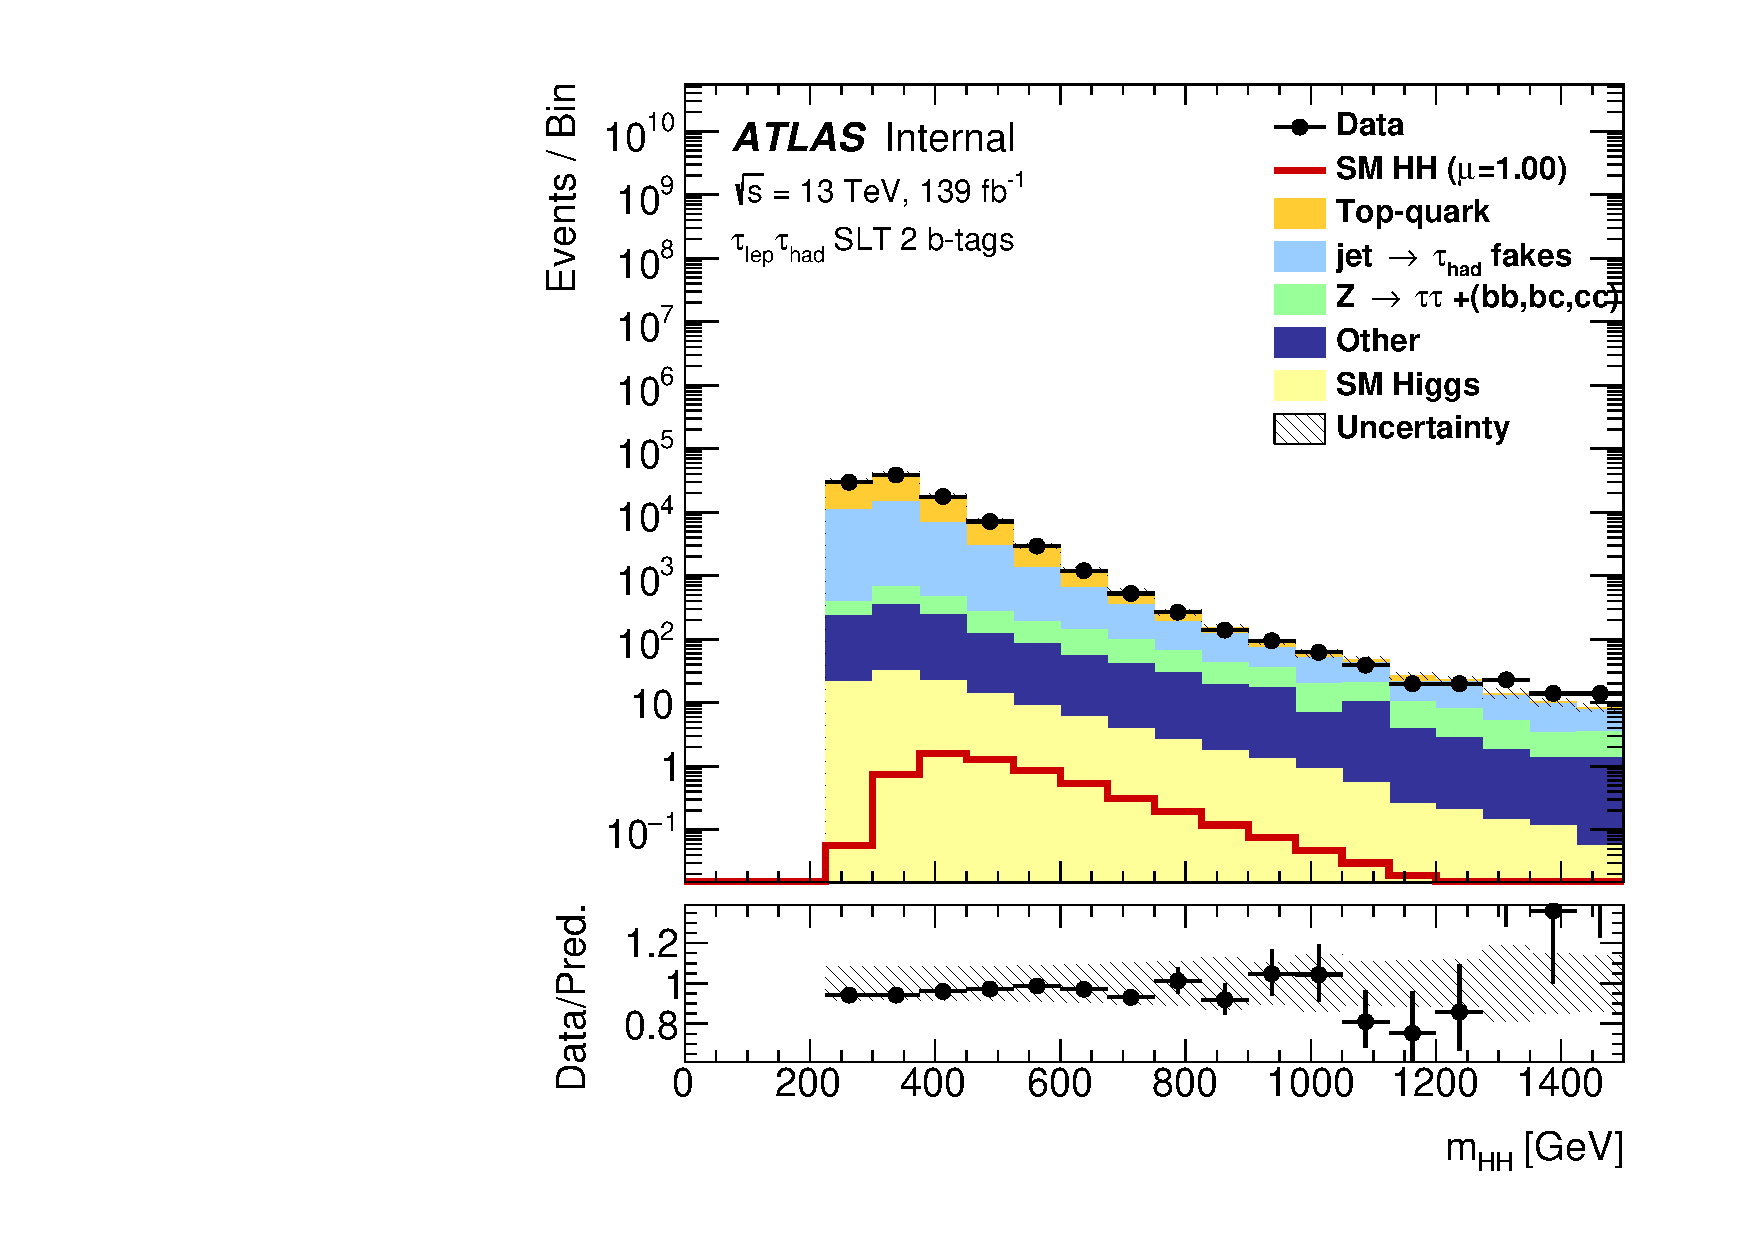
\includegraphics[width=.32\textwidth]{DiHiggs/plots/MVA/SLT/Region_BMin0_incJet1_distMhh_J2_D_T2_SpcTauLH_Y2015_LTT0_L1_Prefitlog.pdf}
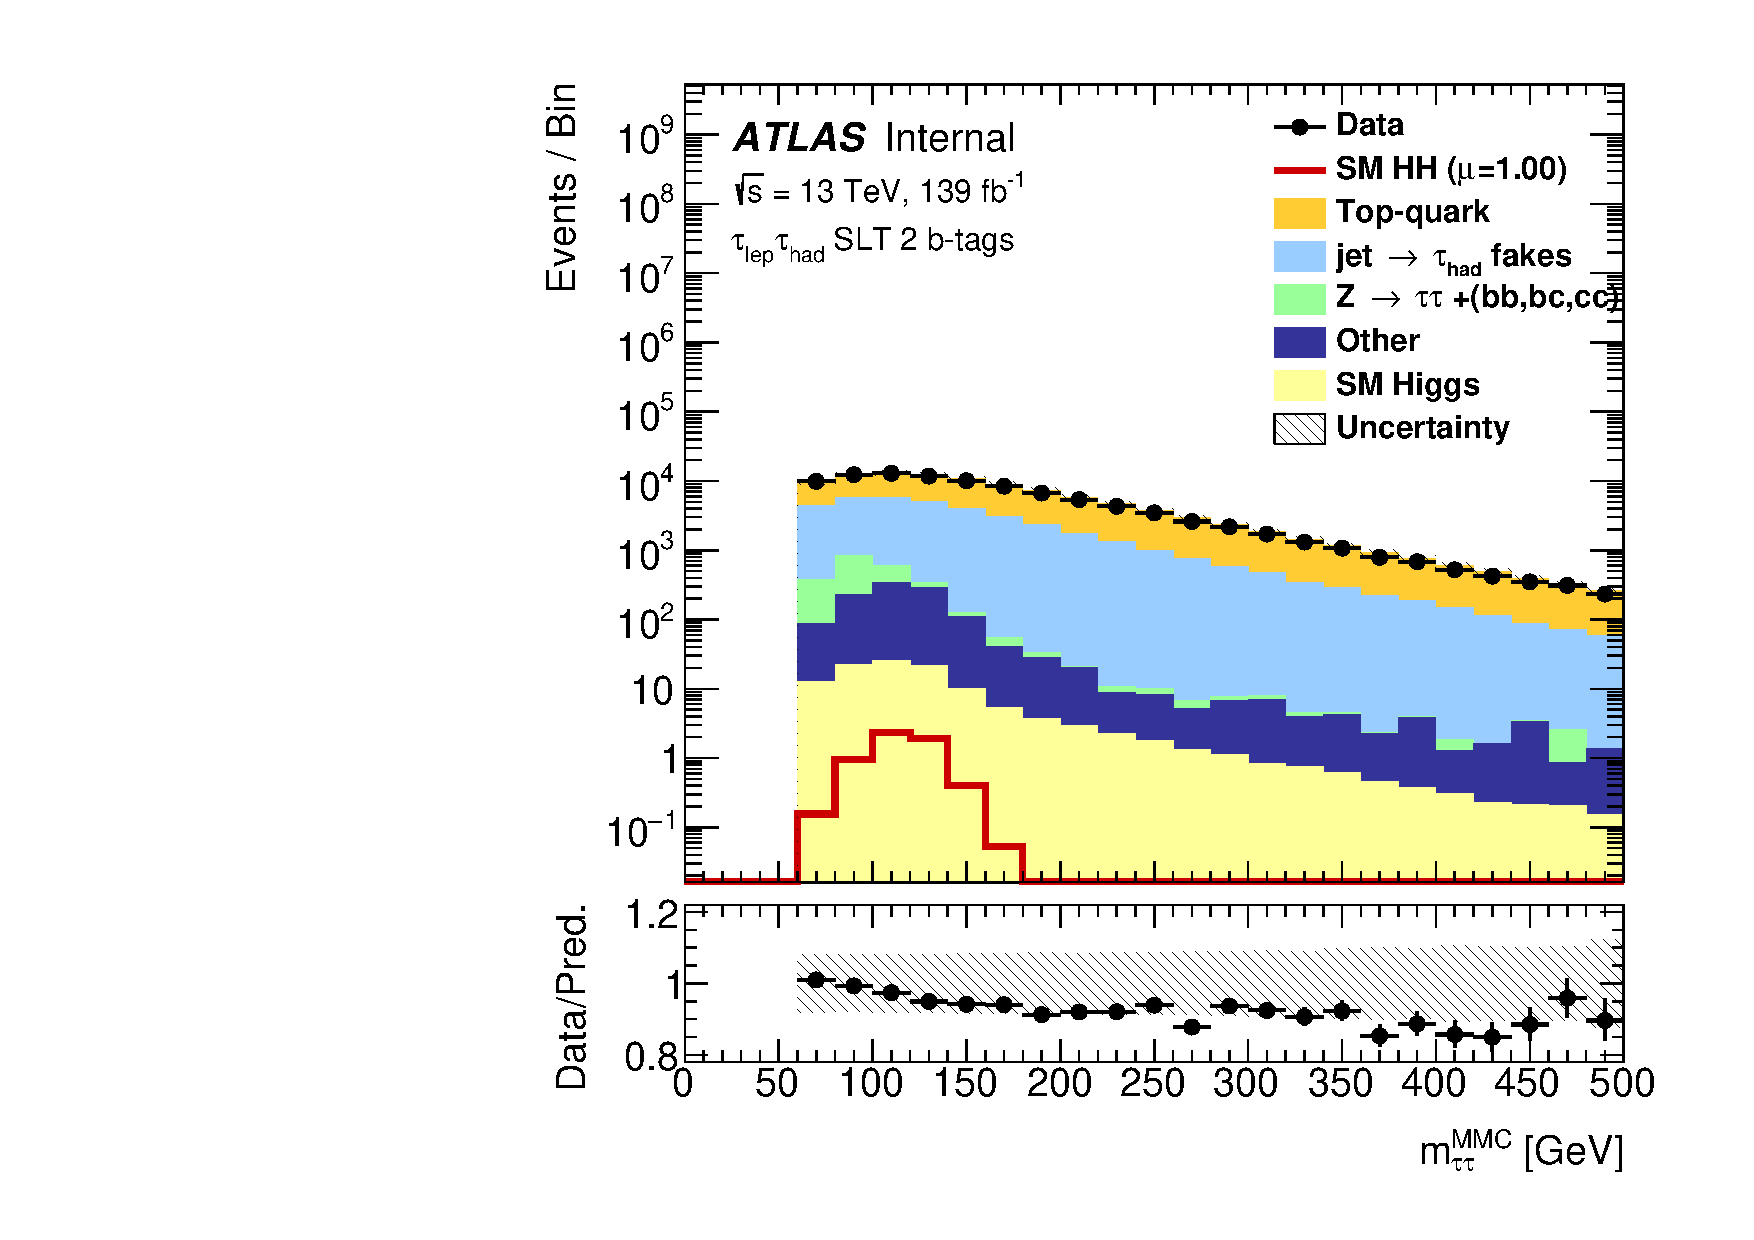
\includegraphics[width=.32\textwidth]{DiHiggs/plots/MVA/SLT/Region_BMin0_incJet1_distmMMC_J2_D_T2_SpcTauLH_Y2015_LTT0_L1_Prefitlog.pdf}
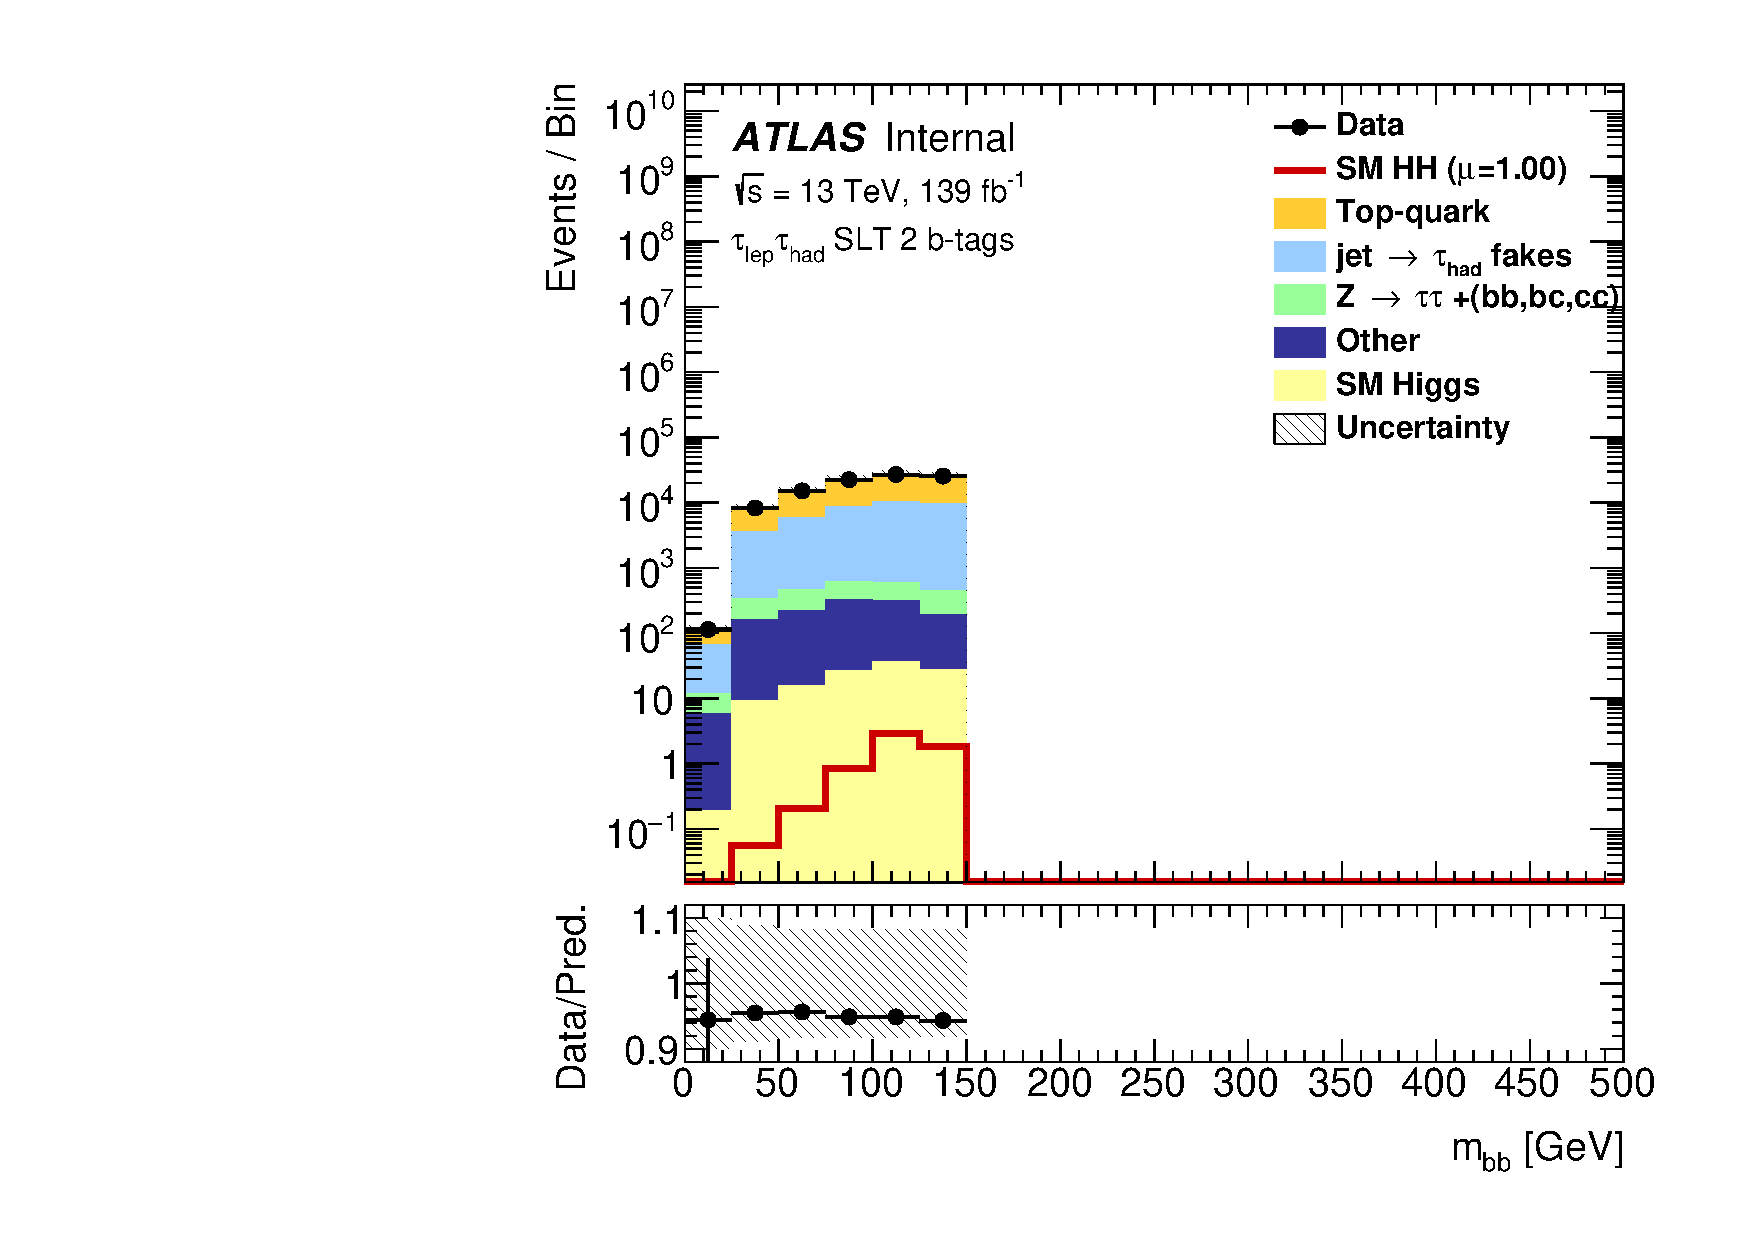
\includegraphics[width=.32\textwidth]{DiHiggs/plots/MVA/SLT/Region_BMin0_incJet1_distmbb_J2_D_T2_SpcTauLH_Y2015_LTT0_L1_Prefitlog.pdf} \\
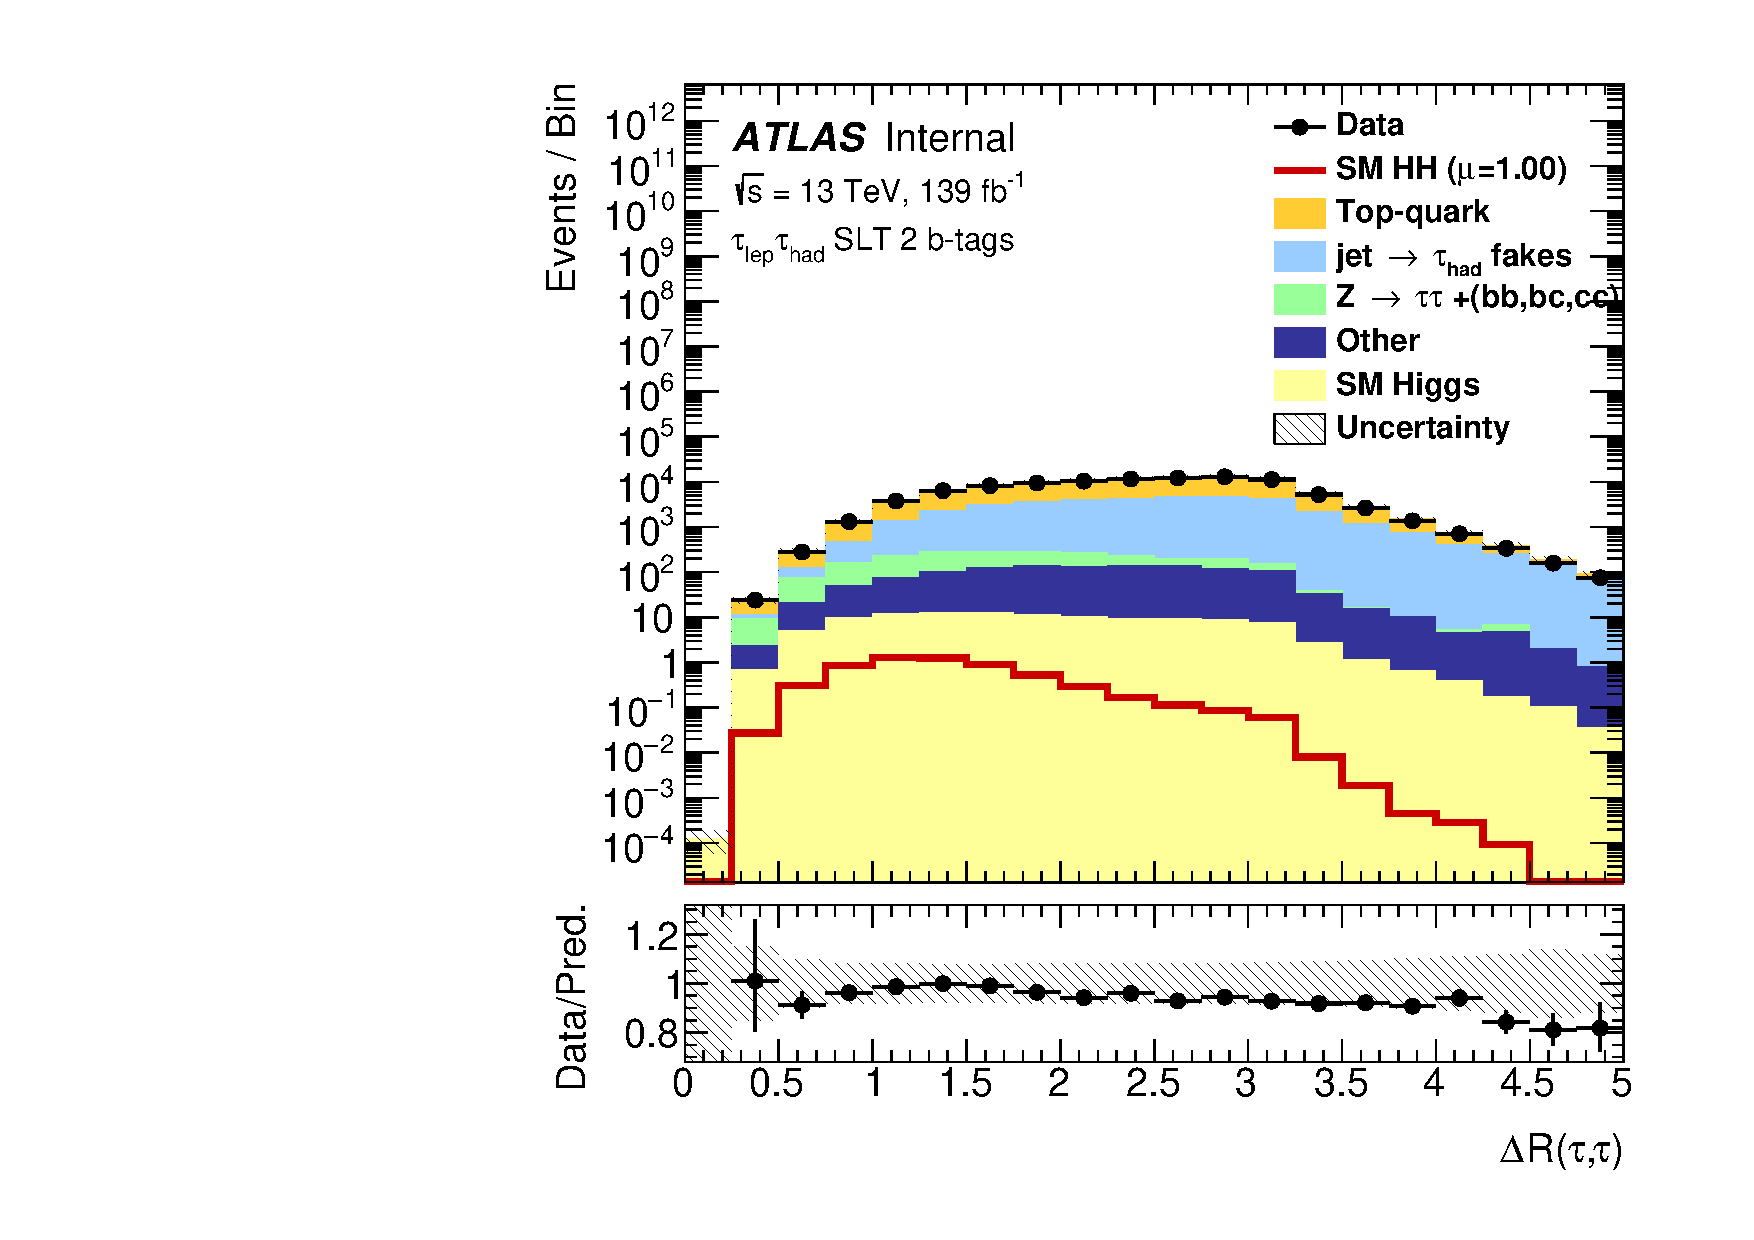
\includegraphics[width=.32\textwidth]{DiHiggs/plots/MVA/SLT/Region_BMin0_incJet1_distDRTauTau_J2_D_T2_SpcTauLH_Y2015_LTT0_L1_Prefitlog.pdf}
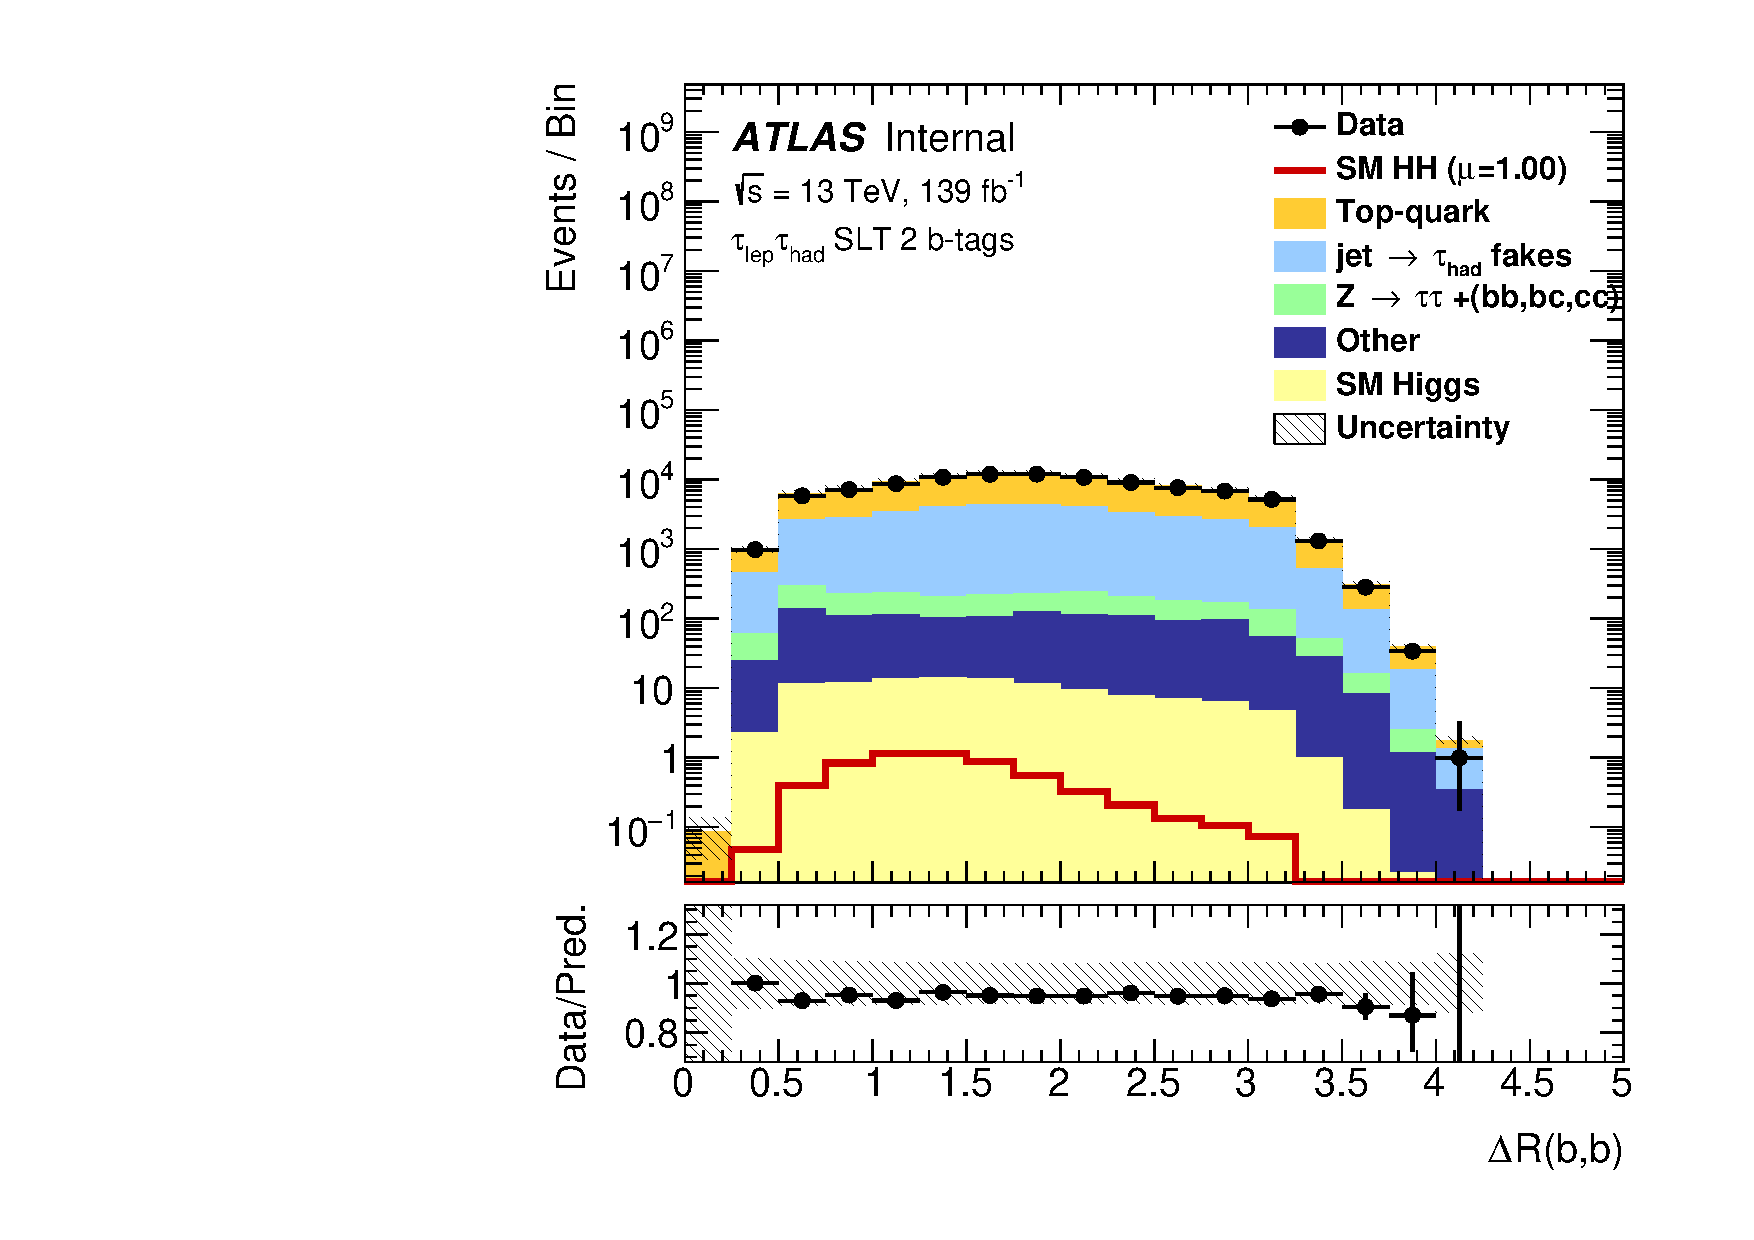
\includegraphics[width=.32\textwidth]{DiHiggs/plots/MVA/SLT/Region_BMin0_incJet1_distdRbb_J2_D_T2_SpcTauLH_Y2015_LTT0_L1_Prefitlog.pdf}
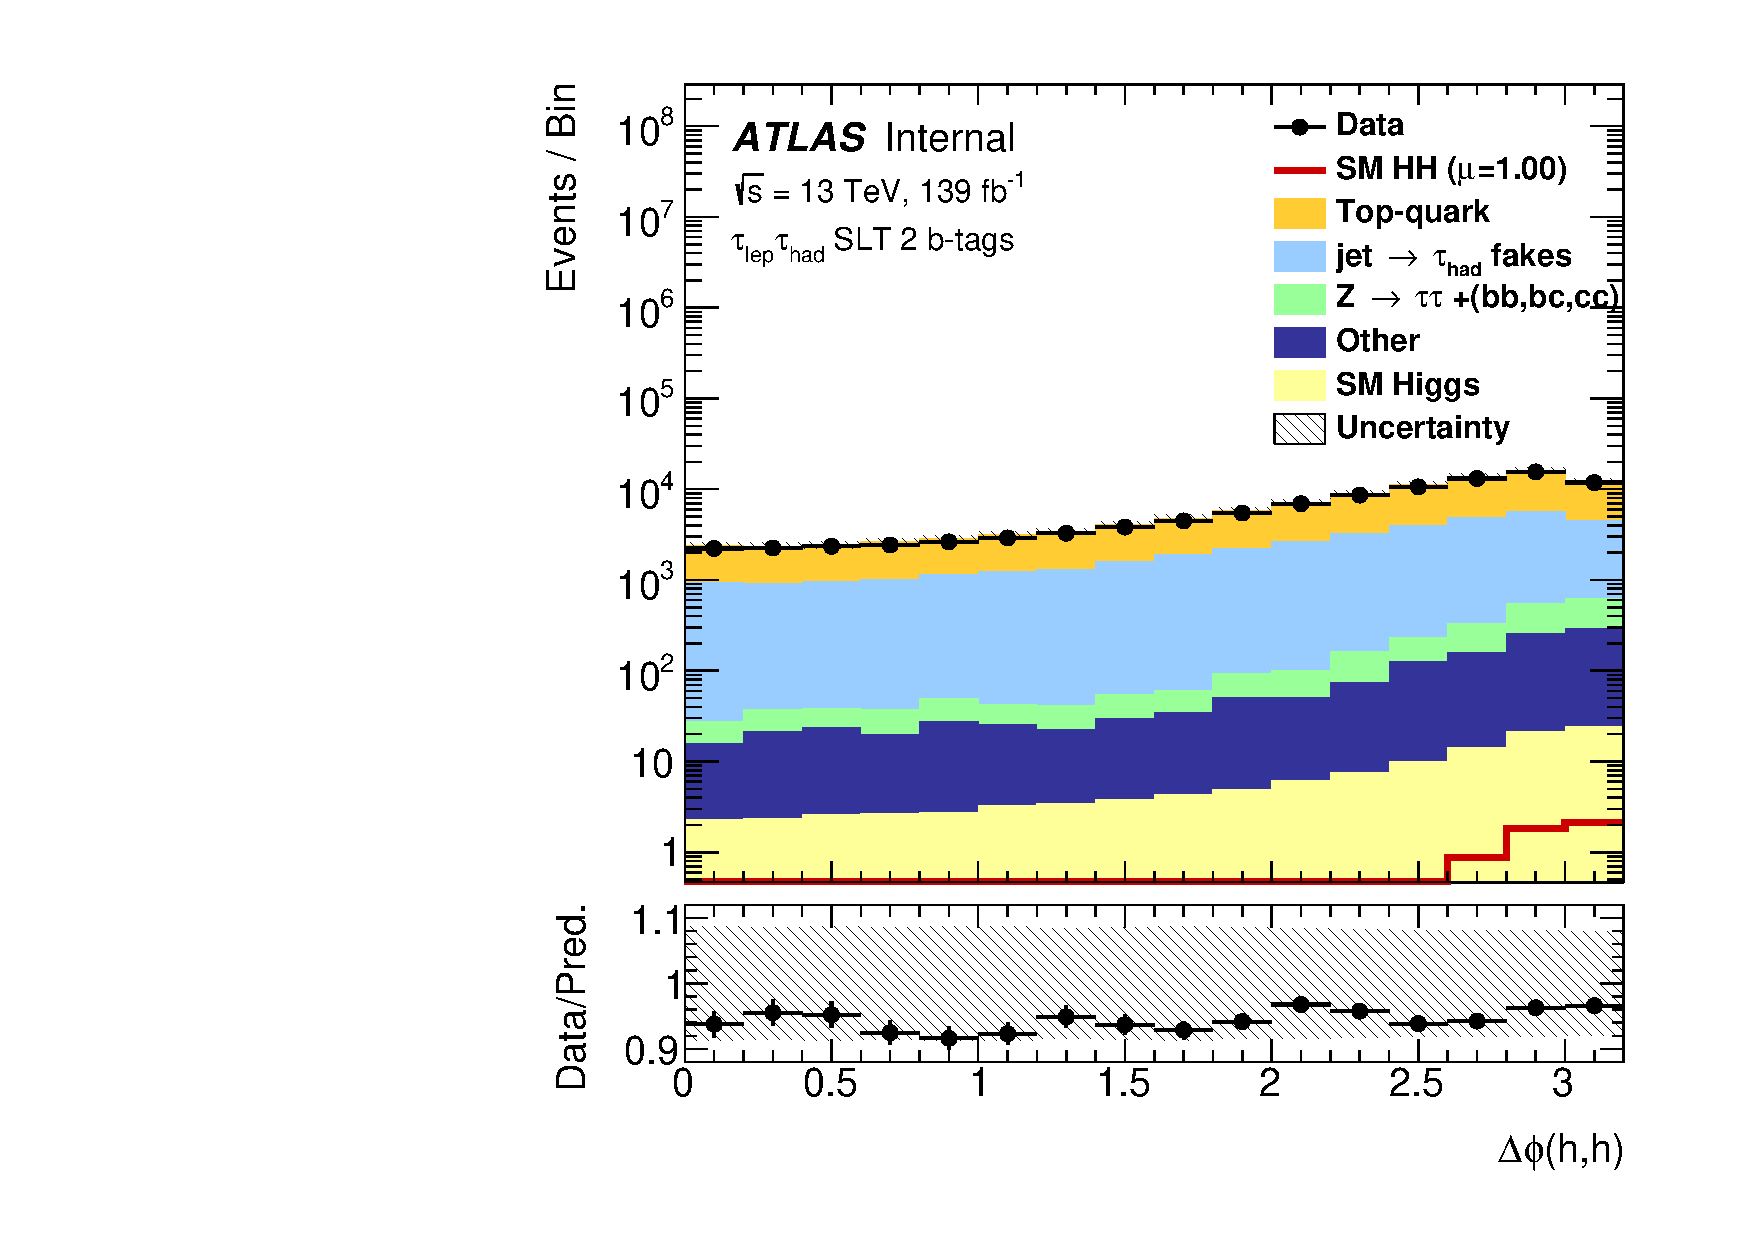
\includegraphics[width=.32\textwidth]{DiHiggs/plots/MVA/SLT/Region_BMin0_incJet1_distdPhiHBB_J2_D_T2_SpcTauLH_Y2015_LTT0_L1_Prefitlog.pdf} \\
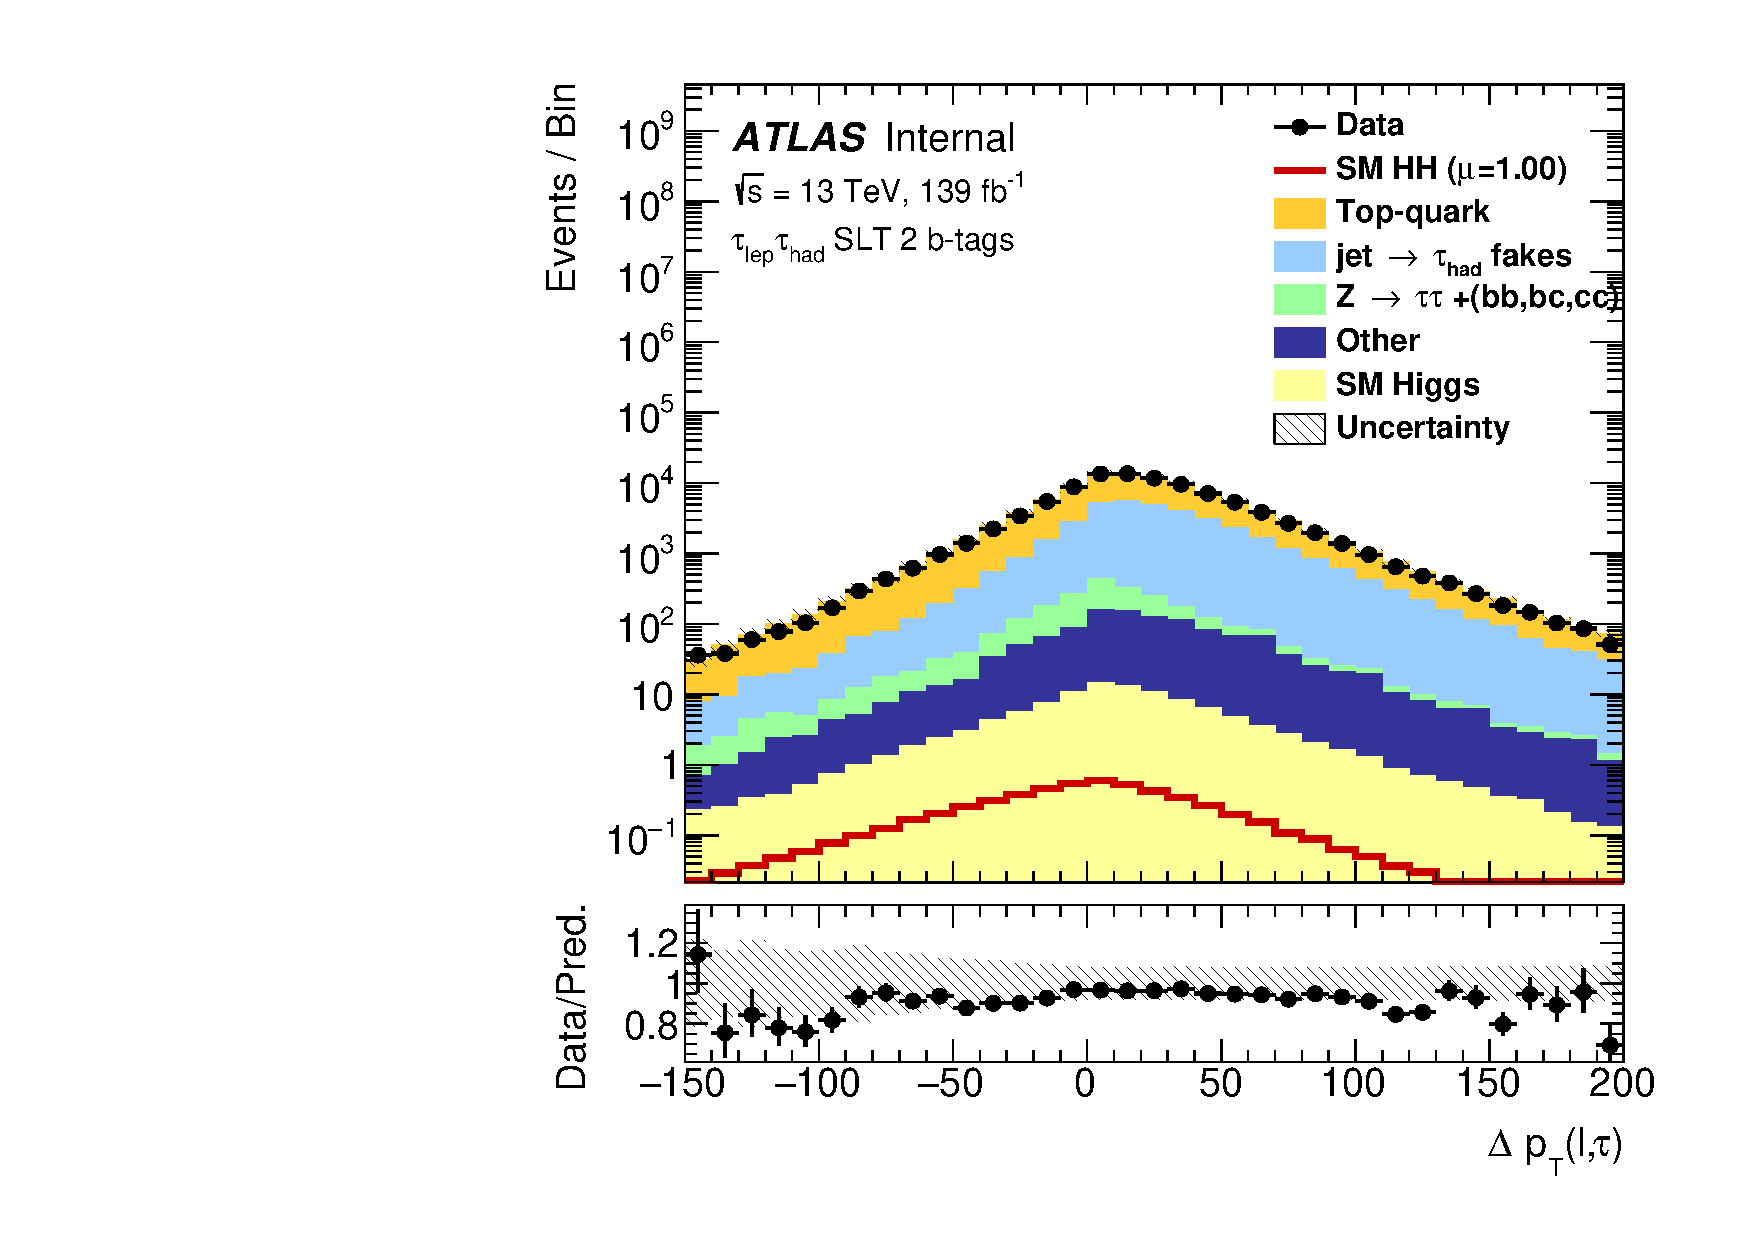
\includegraphics[width=.32\textwidth]{DiHiggs/plots/MVA/SLT/Region_BMin0_incJet1_distdPtLepTau_J2_D_T2_SpcTauLH_Y2015_LTT0_L1_Prefitlog.pdf}
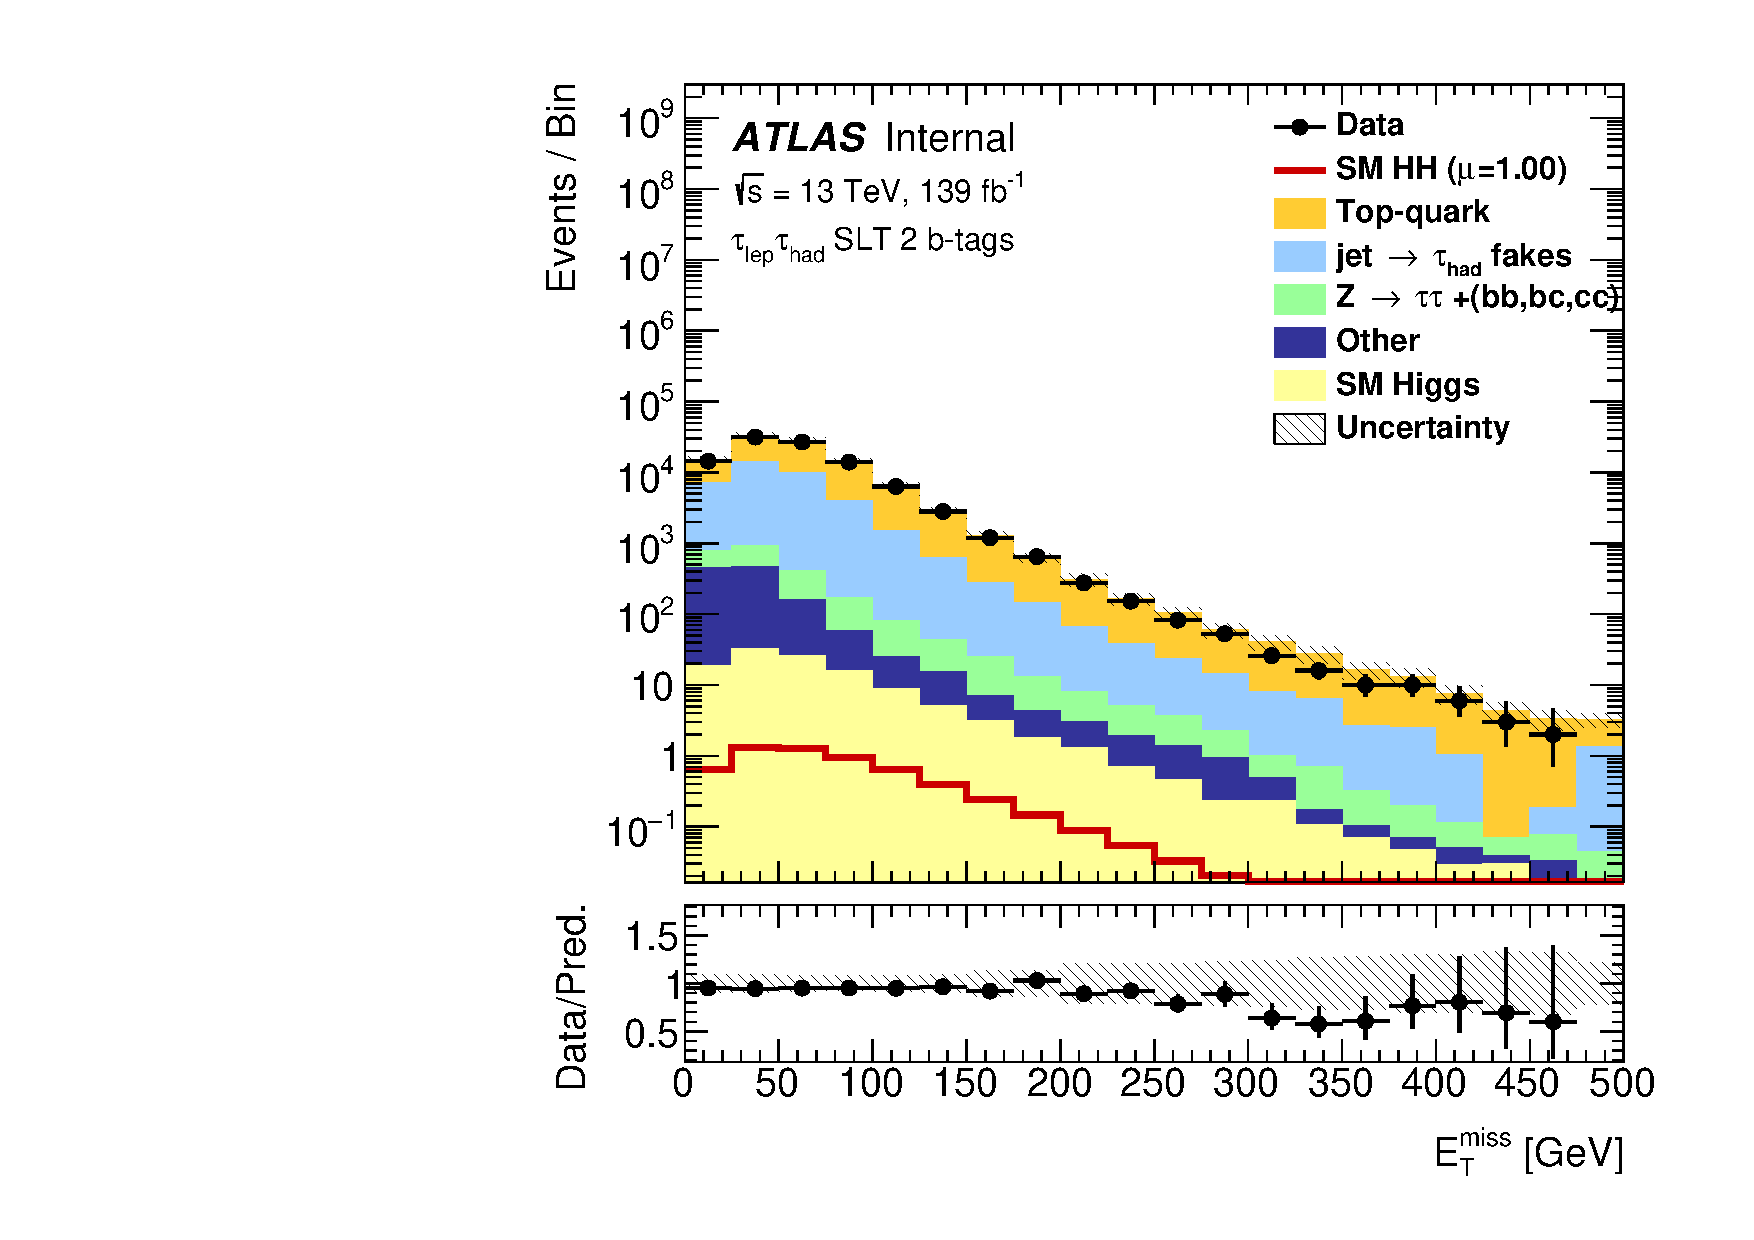
\includegraphics[width=.32\textwidth]{DiHiggs/plots/MVA/SLT/Region_BMin0_incJet1_distMET_J2_D_T2_SpcTauLH_Y2015_LTT0_L1_Prefitlog.pdf}
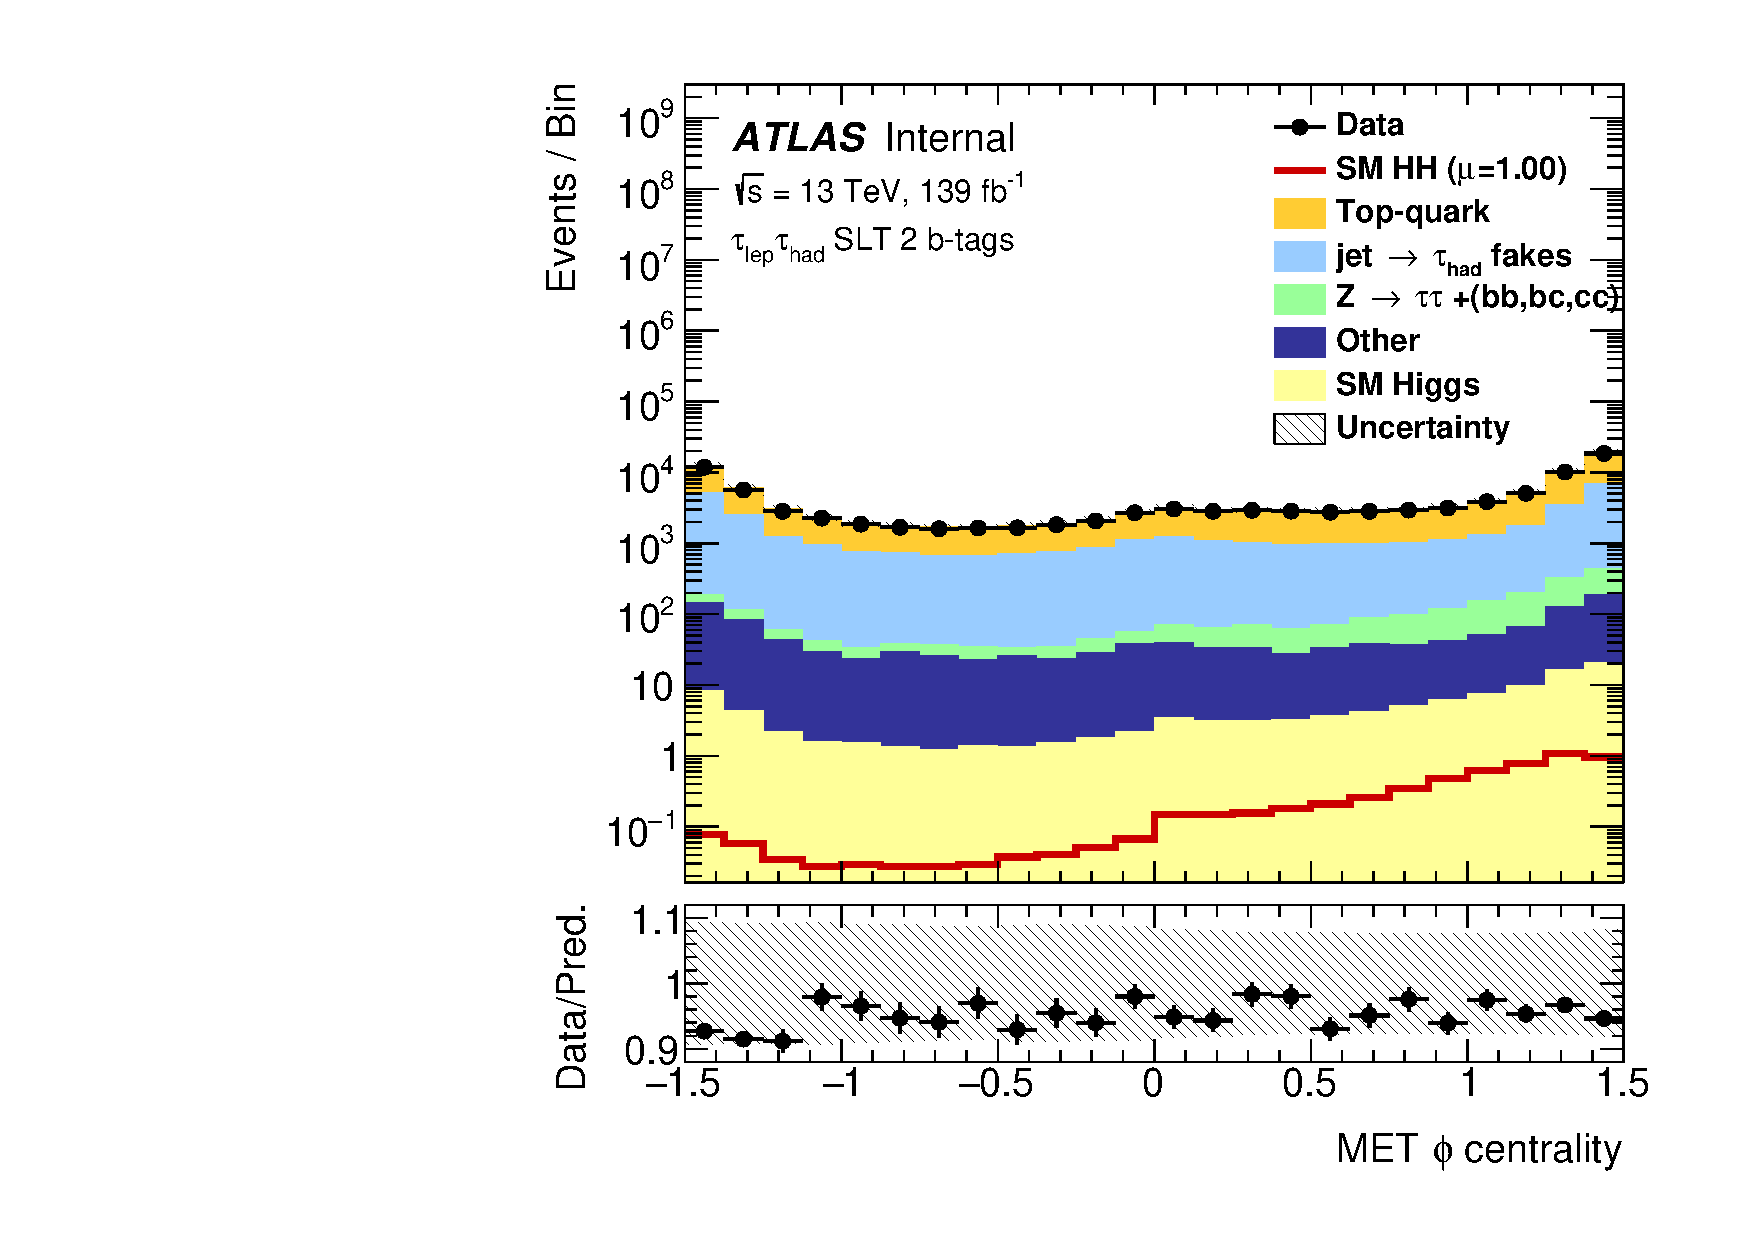
\includegraphics[width=.32\textwidth]{DiHiggs/plots/MVA/SLT/Region_BMin0_incJet1_distMETCent_J2_D_T2_SpcTauLH_Y2015_LTT0_L1_Prefitlog.pdf} \\
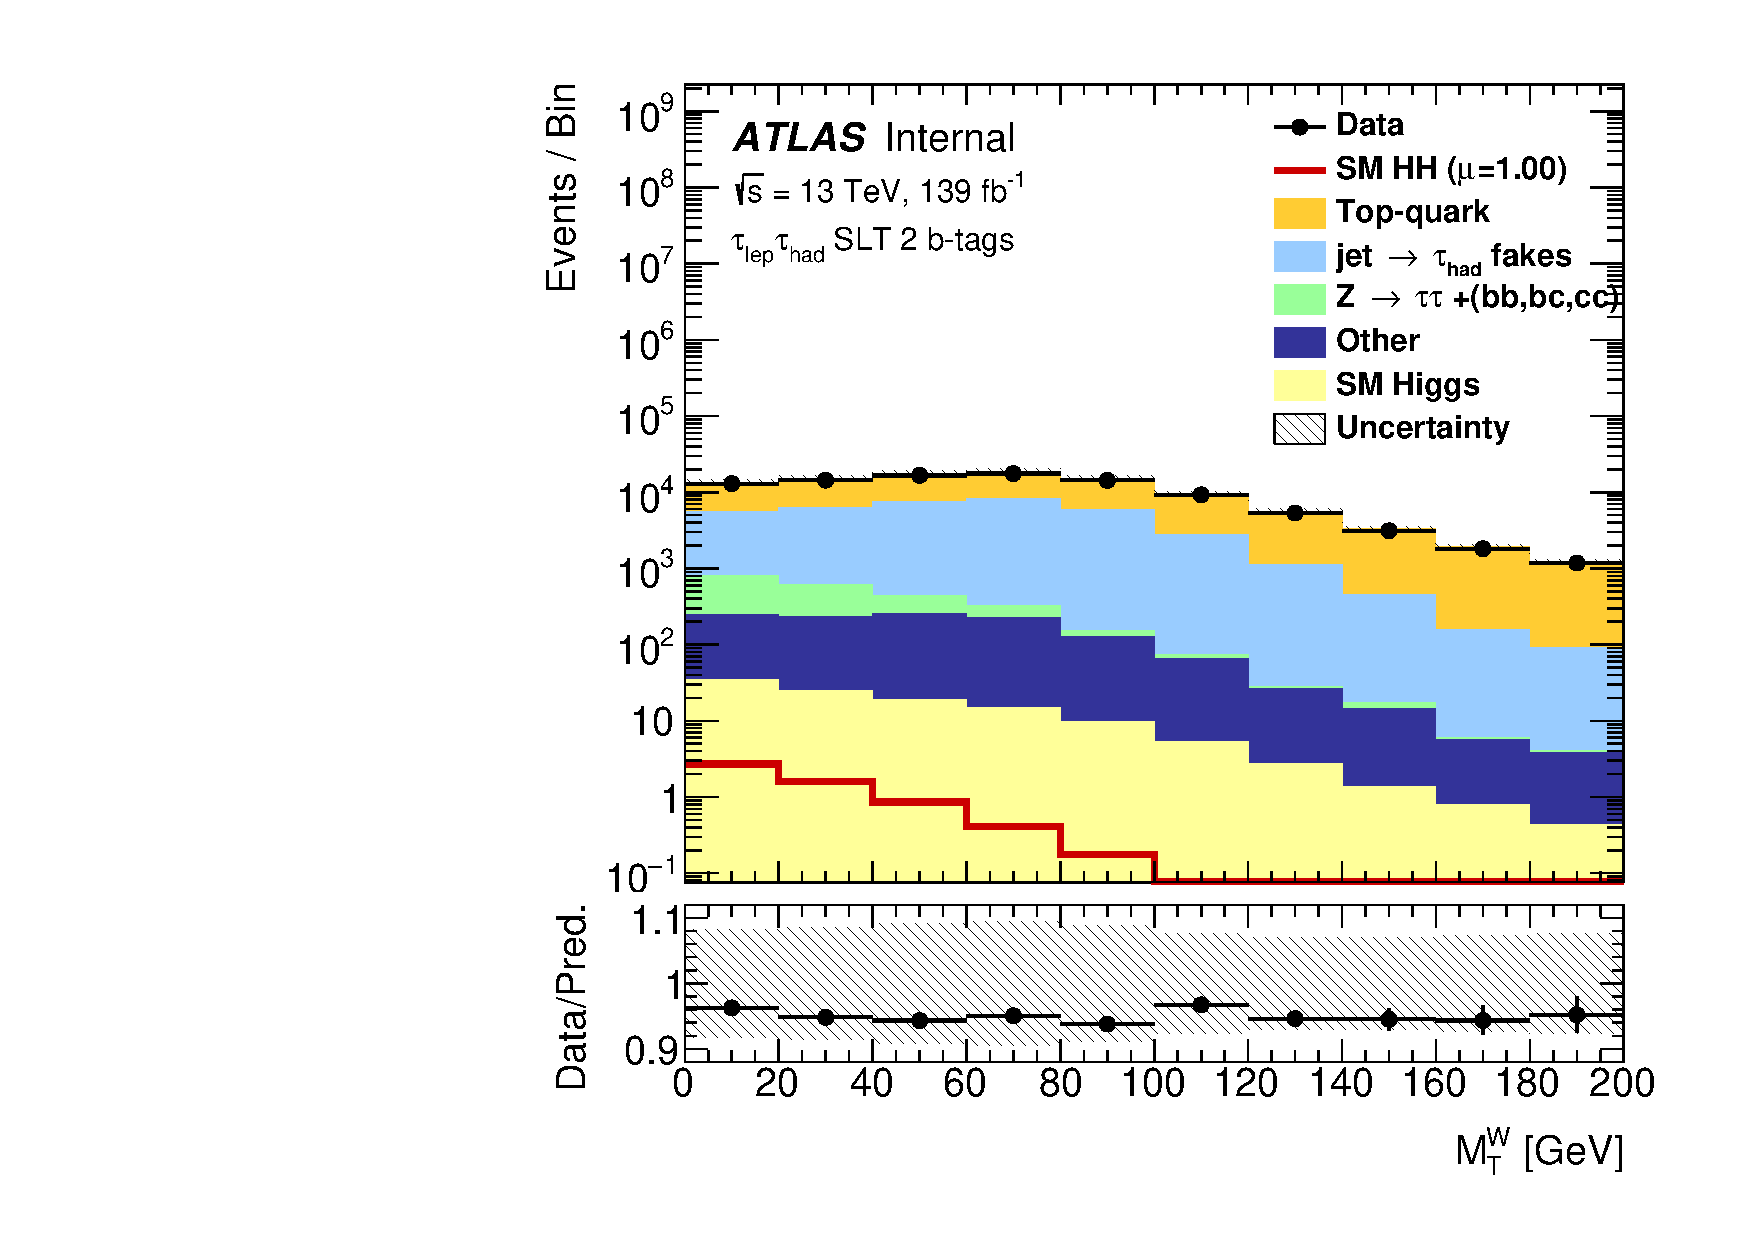
\includegraphics[width=.32\textwidth]{DiHiggs/plots/MVA/SLT/Region_BMin0_incJet1_distMtW_J2_D_T2_SpcTauLH_Y2015_LTT0_L1_Prefitlog.pdf}
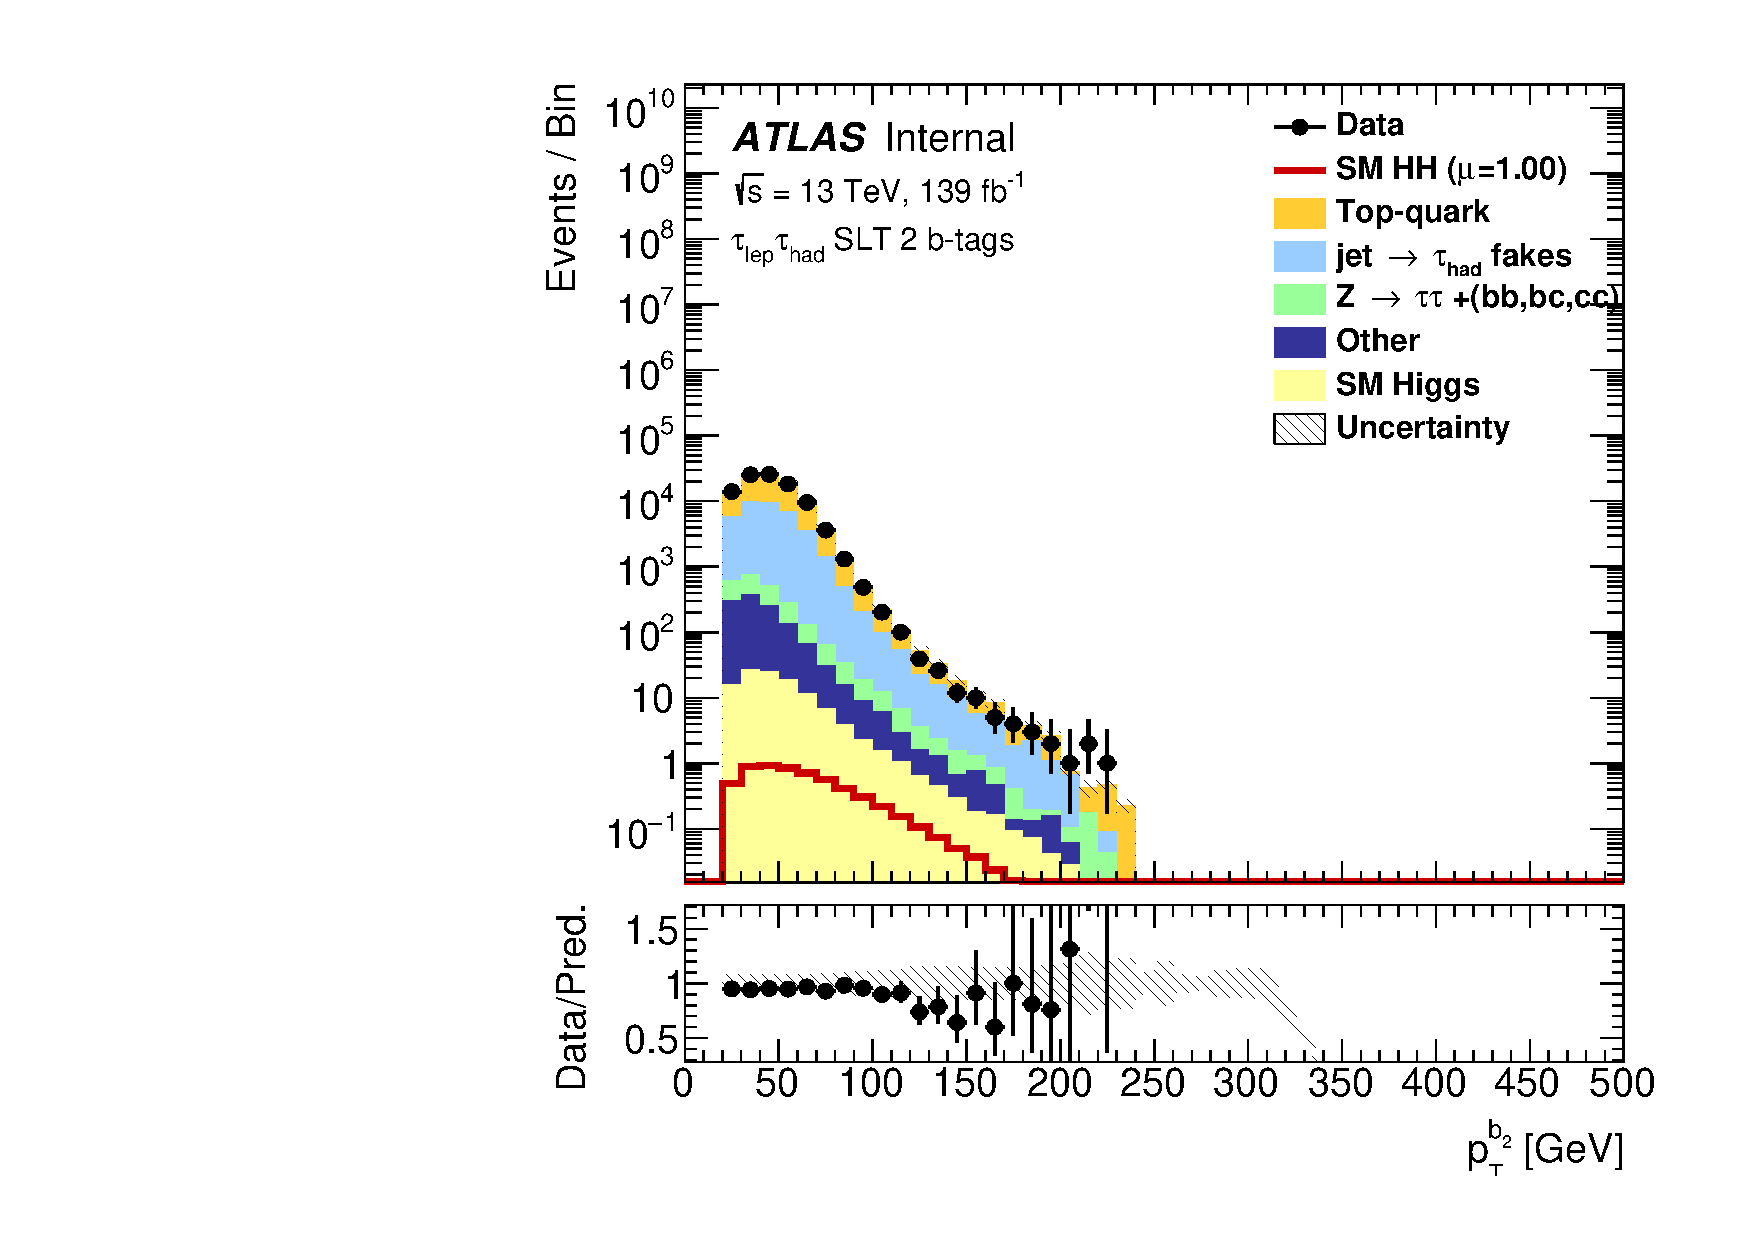
\includegraphics[width=.32\textwidth]{DiHiggs/plots/MVA/SLT/Region_BMin0_incJet1_distpTB2_J2_D_T2_SpcTauLH_Y2015_LTT0_L1_Prefitlog.pdf}
\caption{Pre-fit PNN/NN input variable distributions for the SLT signal region.}
\label{fig:lephadmvainputsslt}
\end{figure}
  
  
\begin{figure}
\centering
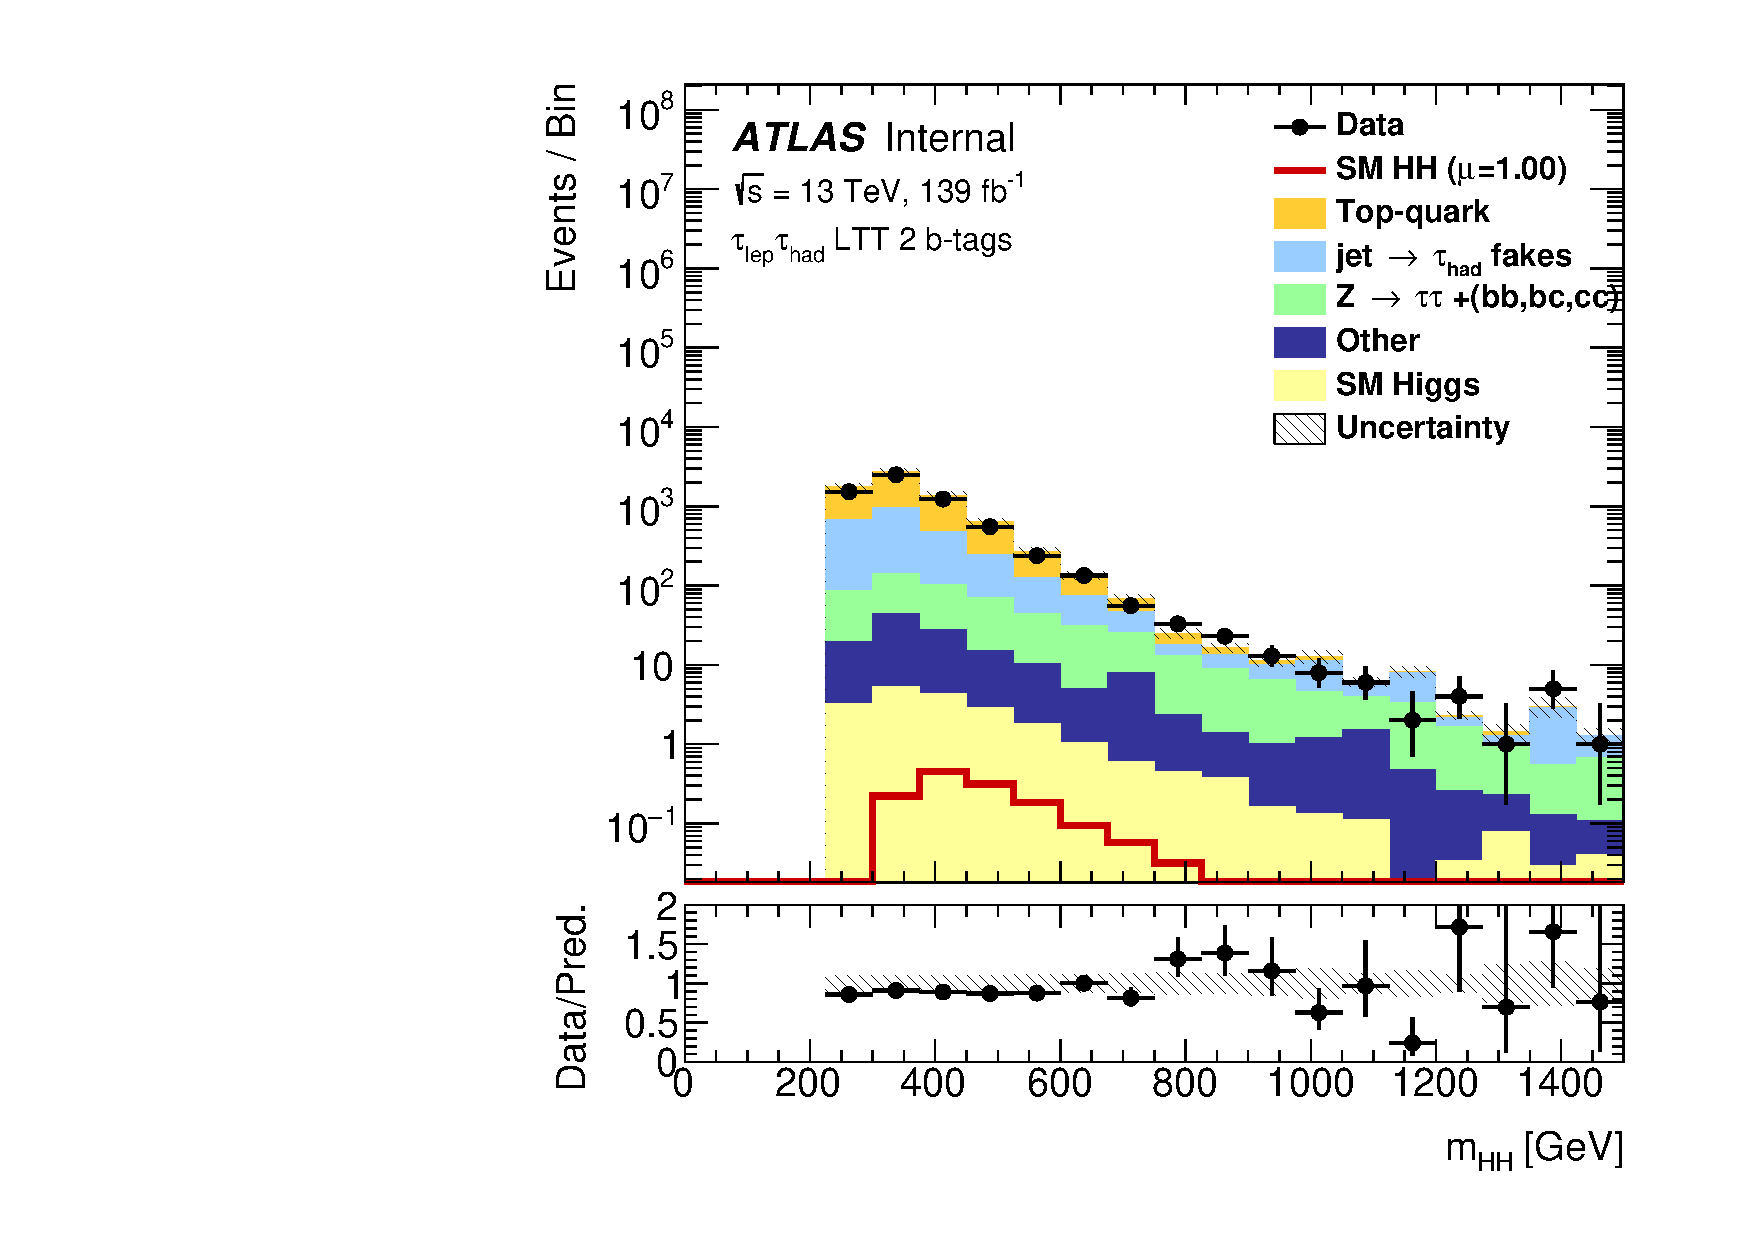
\includegraphics[width=.32\textwidth]{DiHiggs/plots/MVA/LTT/Region_BMin0_incJet1_distMhh_J2_D_T2_SpcTauLH_Y2015_LTT1_L1_Prefitlog.pdf}
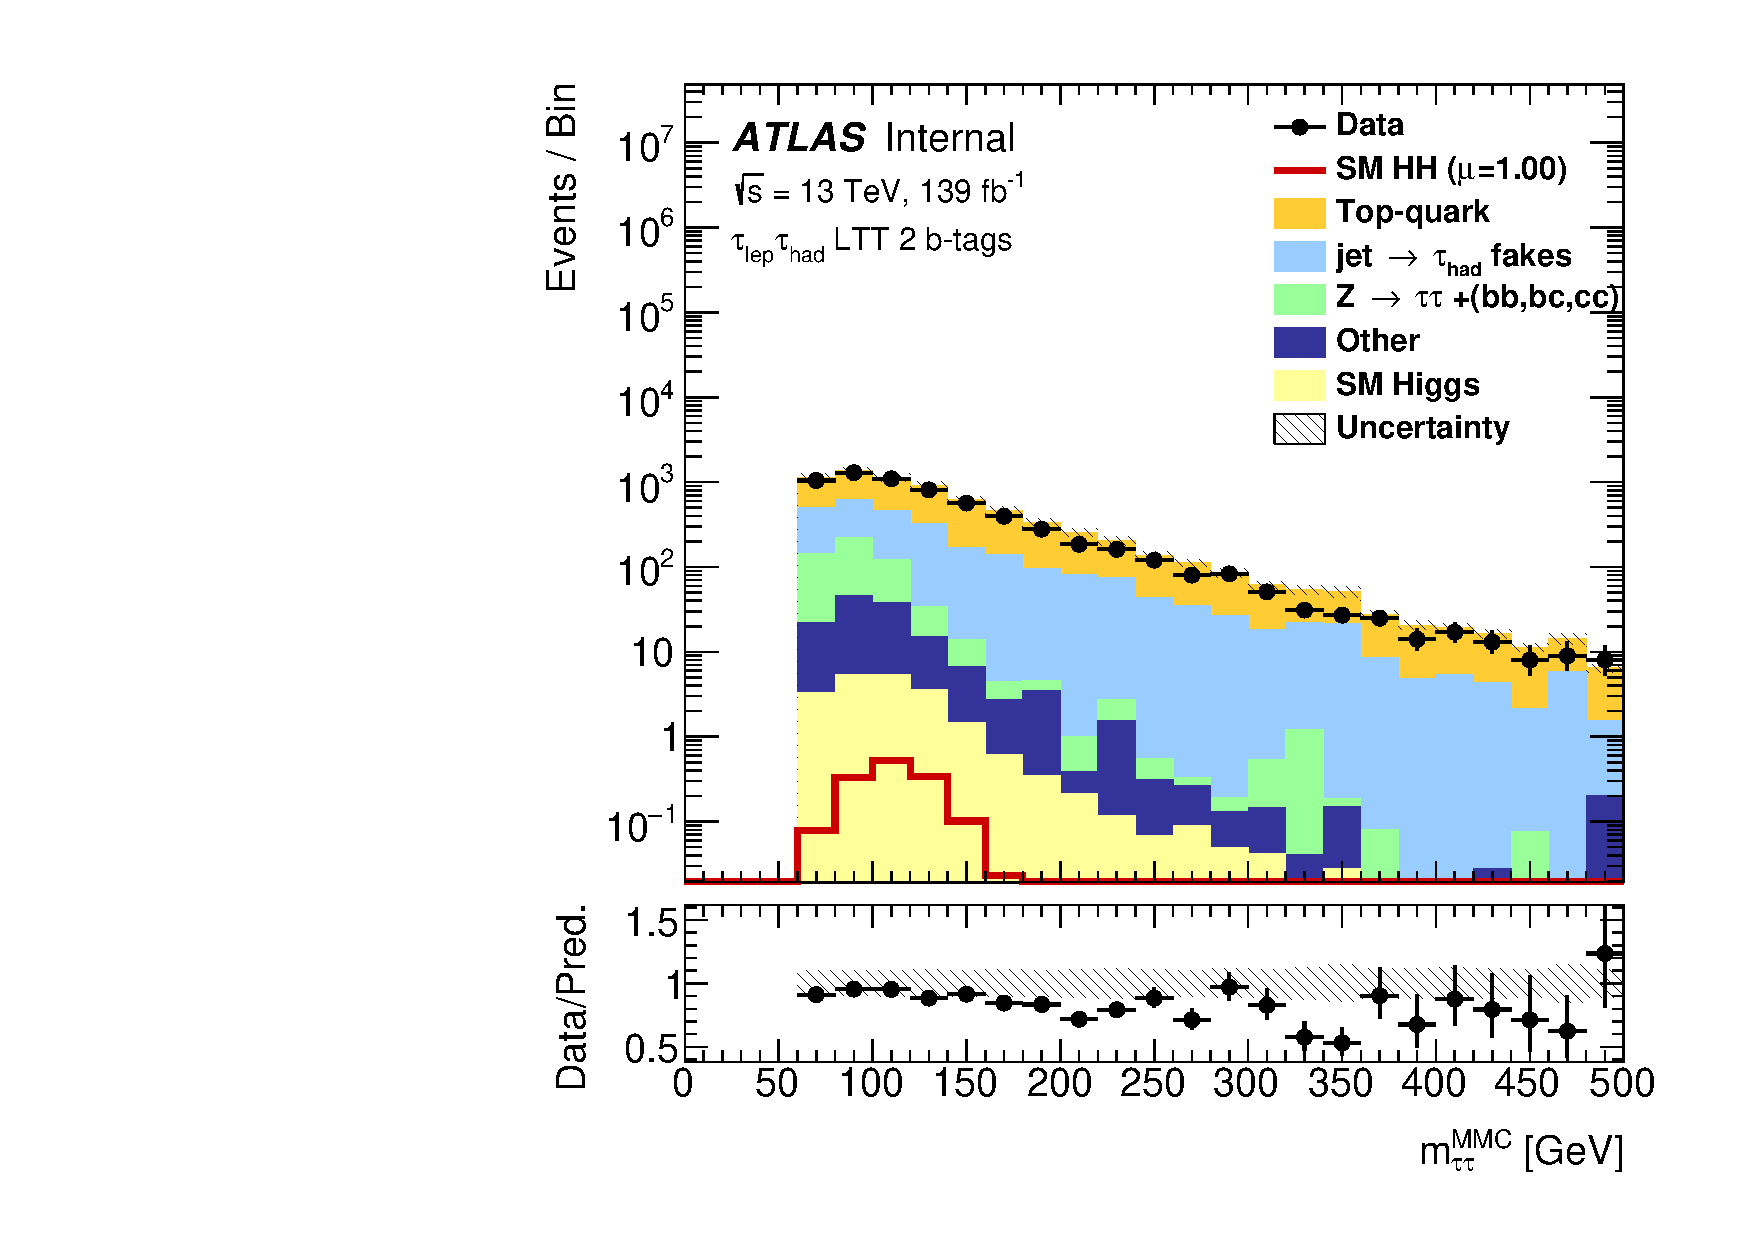
\includegraphics[width=.32\textwidth]{DiHiggs/plots/MVA/LTT/Region_BMin0_incJet1_distmMMC_J2_D_T2_SpcTauLH_Y2015_LTT1_L1_Prefitlog.pdf} 
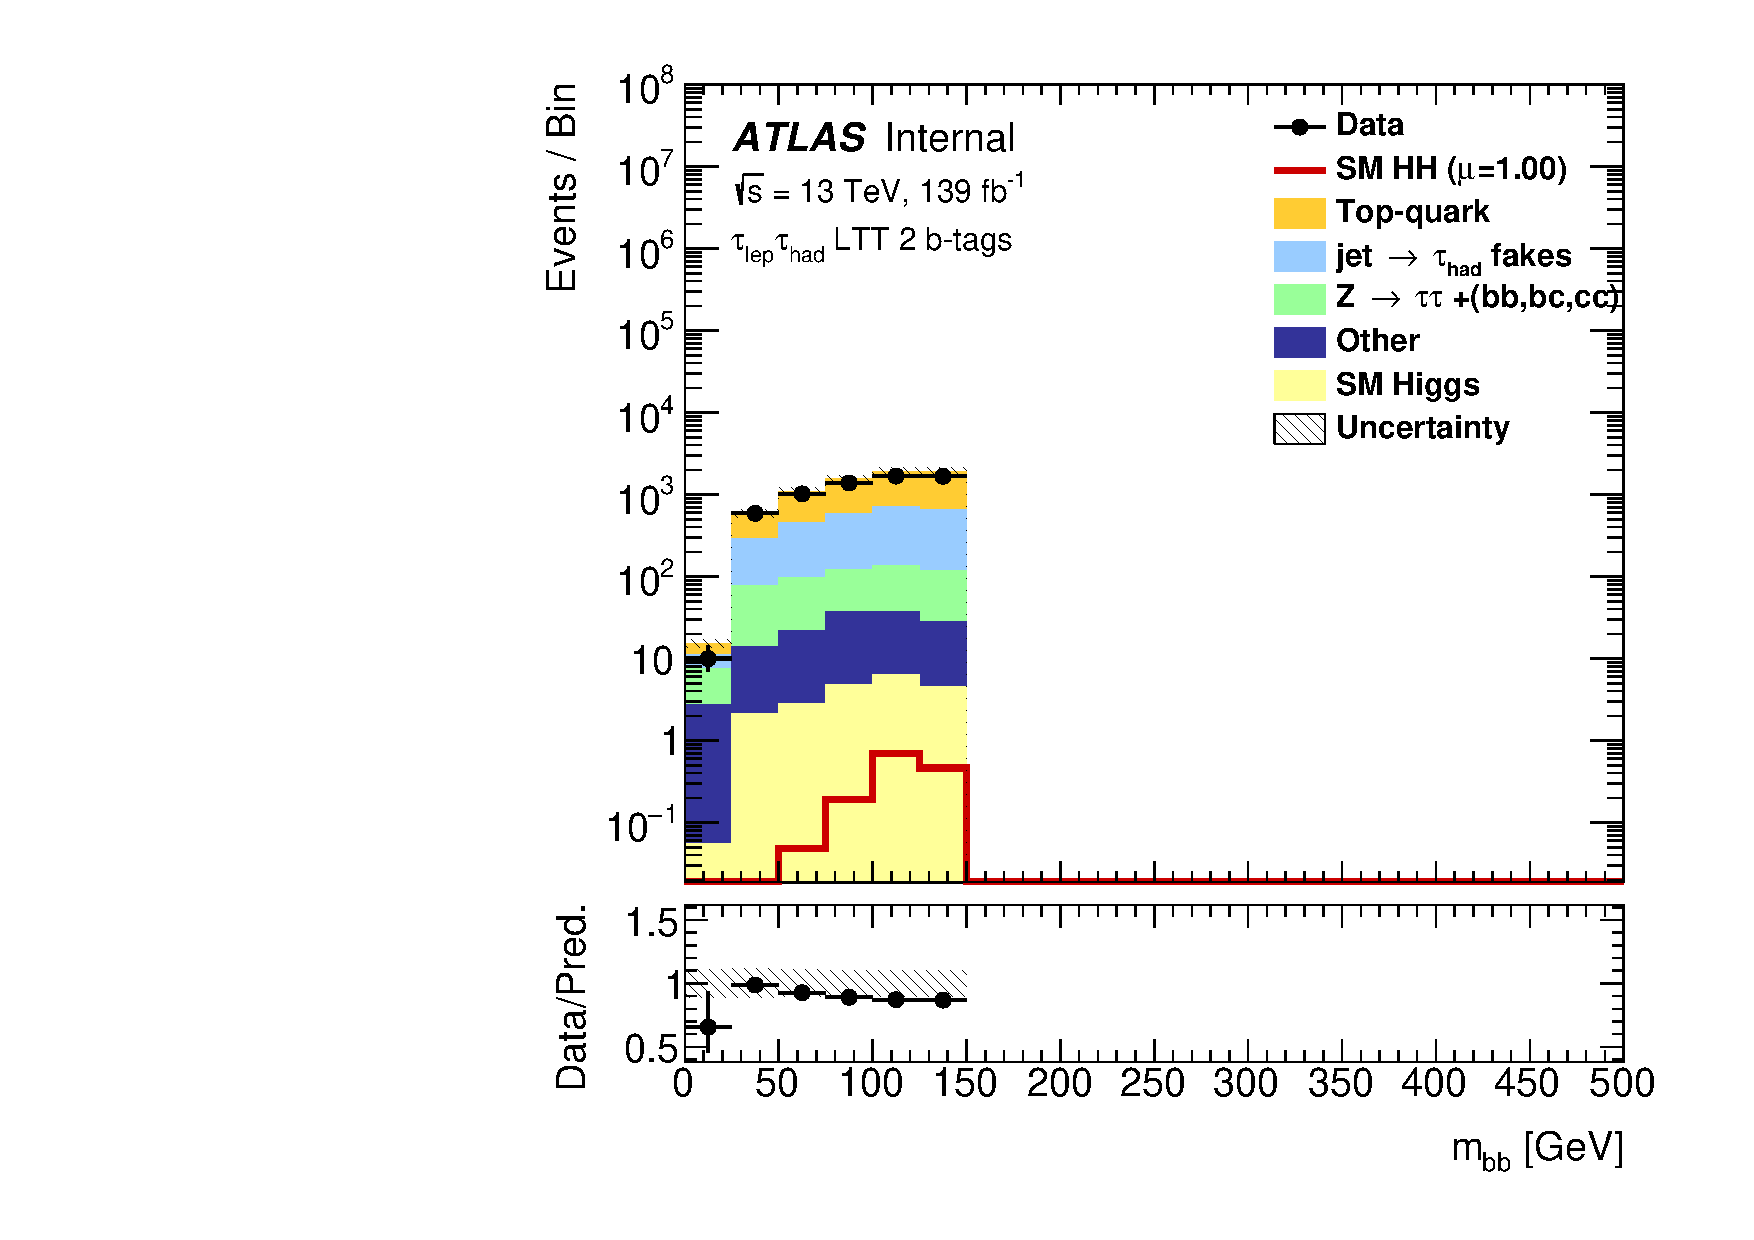
\includegraphics[width=.32\textwidth]{DiHiggs/plots/MVA/LTT/Region_BMin0_incJet1_distmbb_J2_D_T2_SpcTauLH_Y2015_LTT1_L1_Prefitlog.pdf} \\
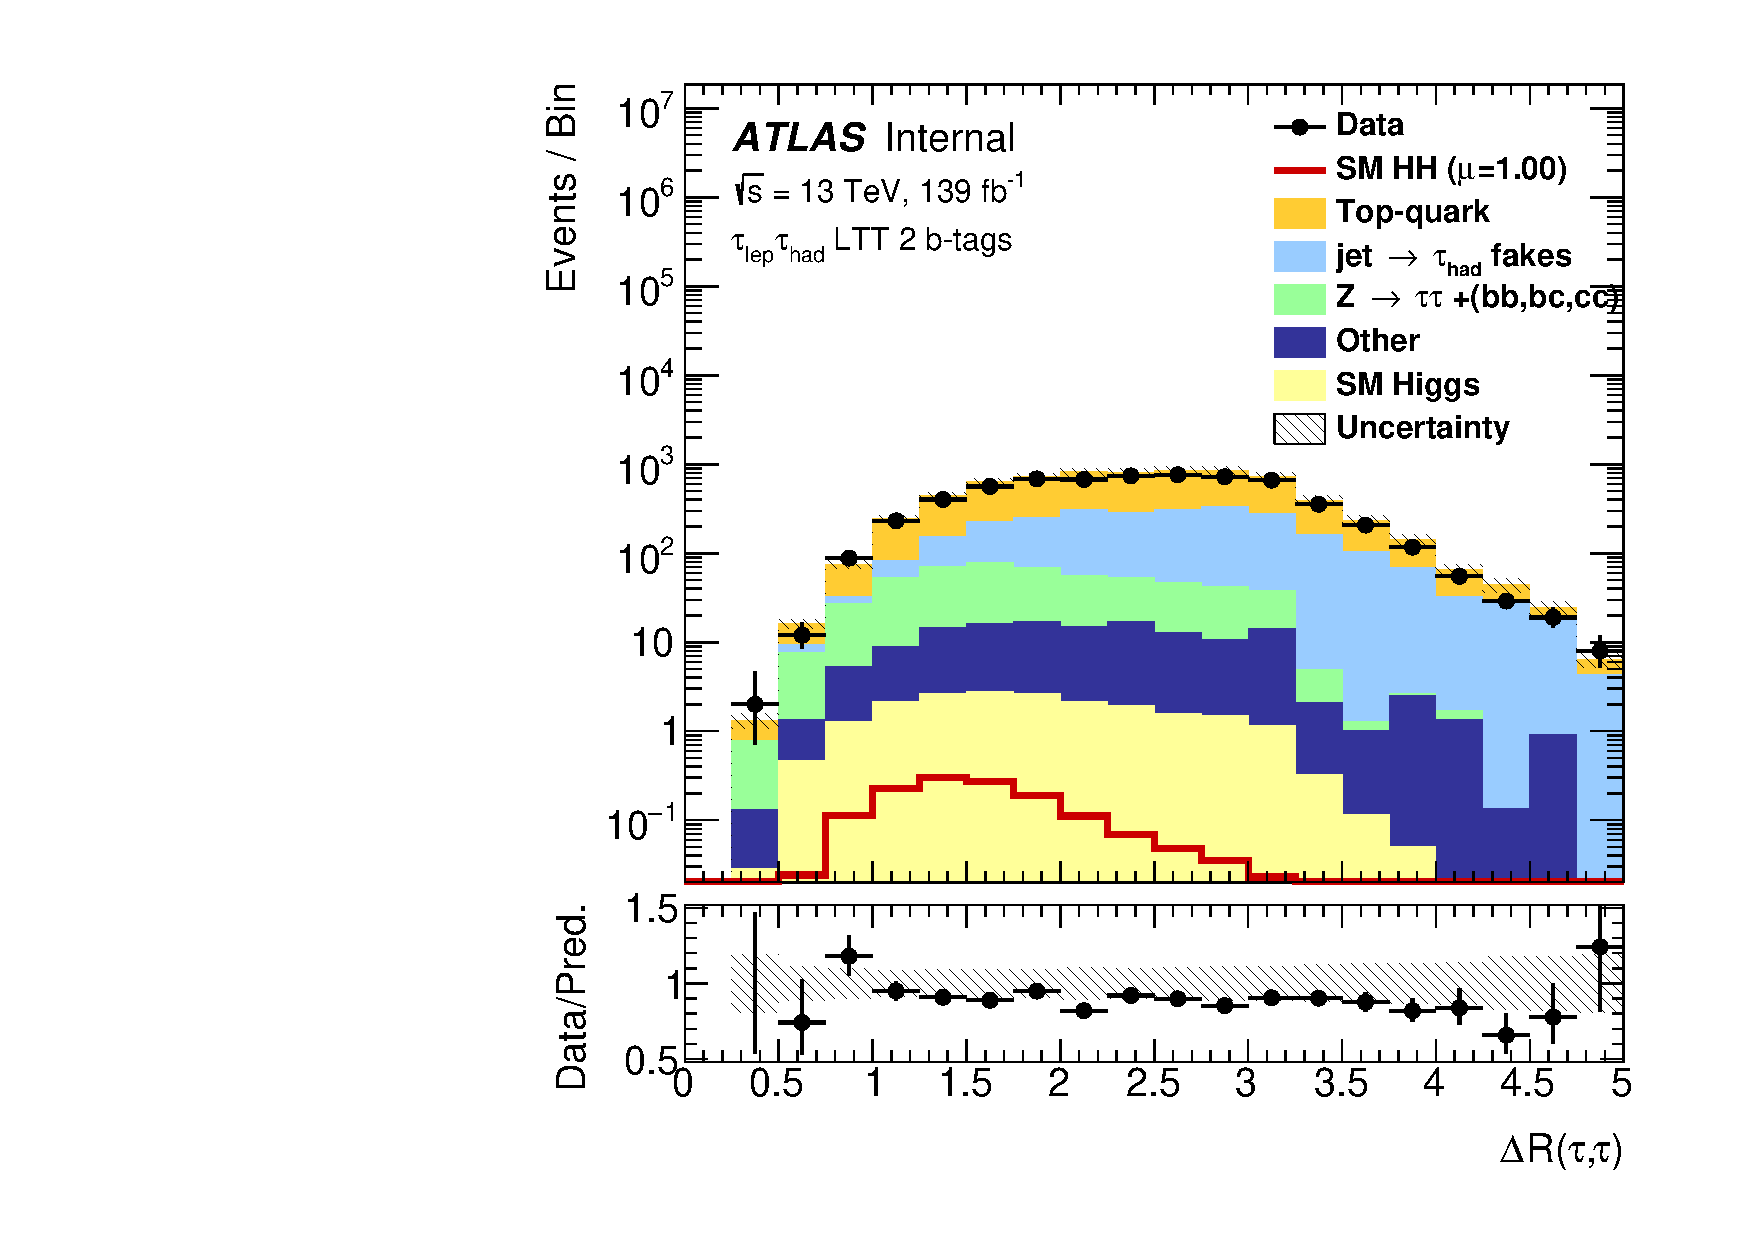
\includegraphics[width=.32\textwidth]{DiHiggs/plots/MVA/LTT/Region_BMin0_incJet1_distDRTauTau_J2_D_T2_SpcTauLH_Y2015_LTT1_L1_Prefitlog.pdf} 
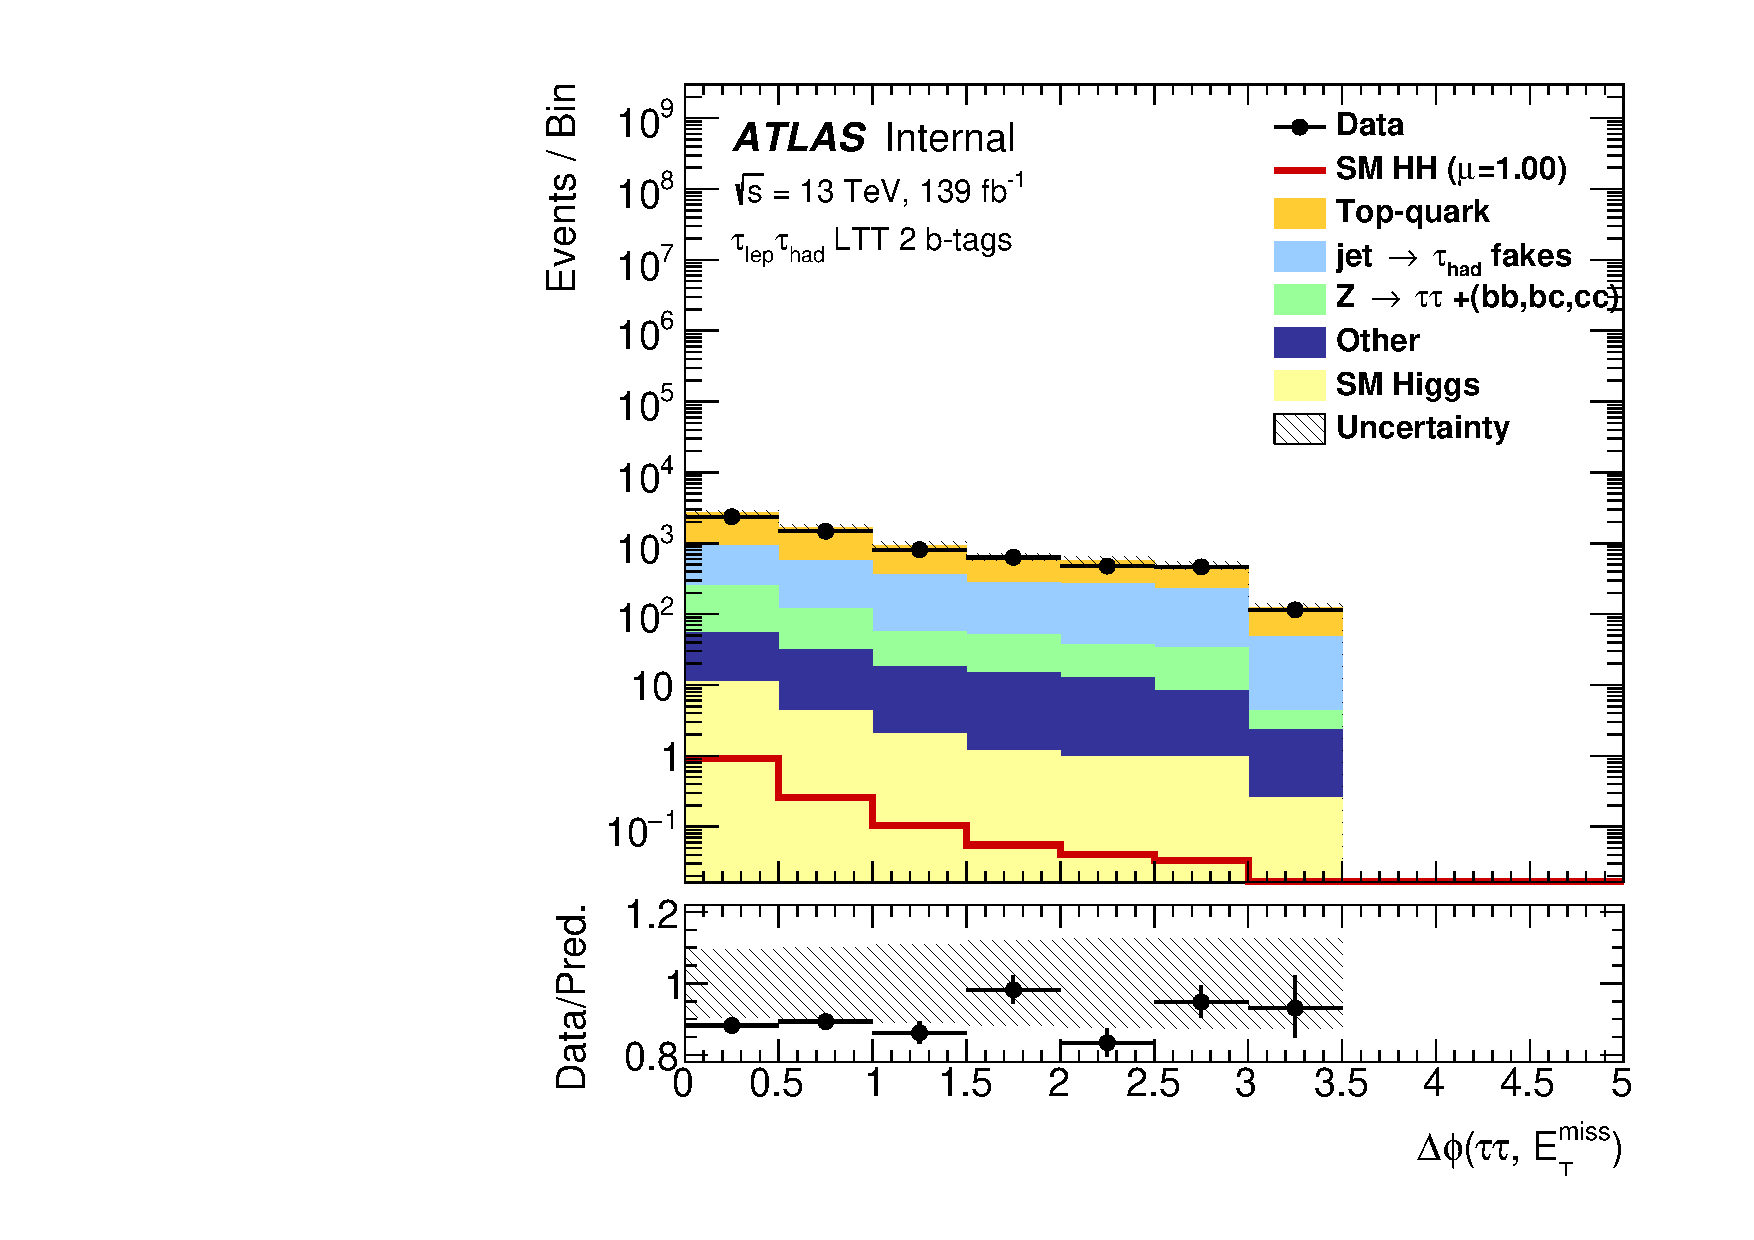
\includegraphics[width=.32\textwidth]{DiHiggs/plots/MVA/LTT/Region_BMin0_incJet1_distdPhiHttMET_J2_D_T2_SpcTauLH_Y2015_LTT1_L1_Prefitlog.pdf}
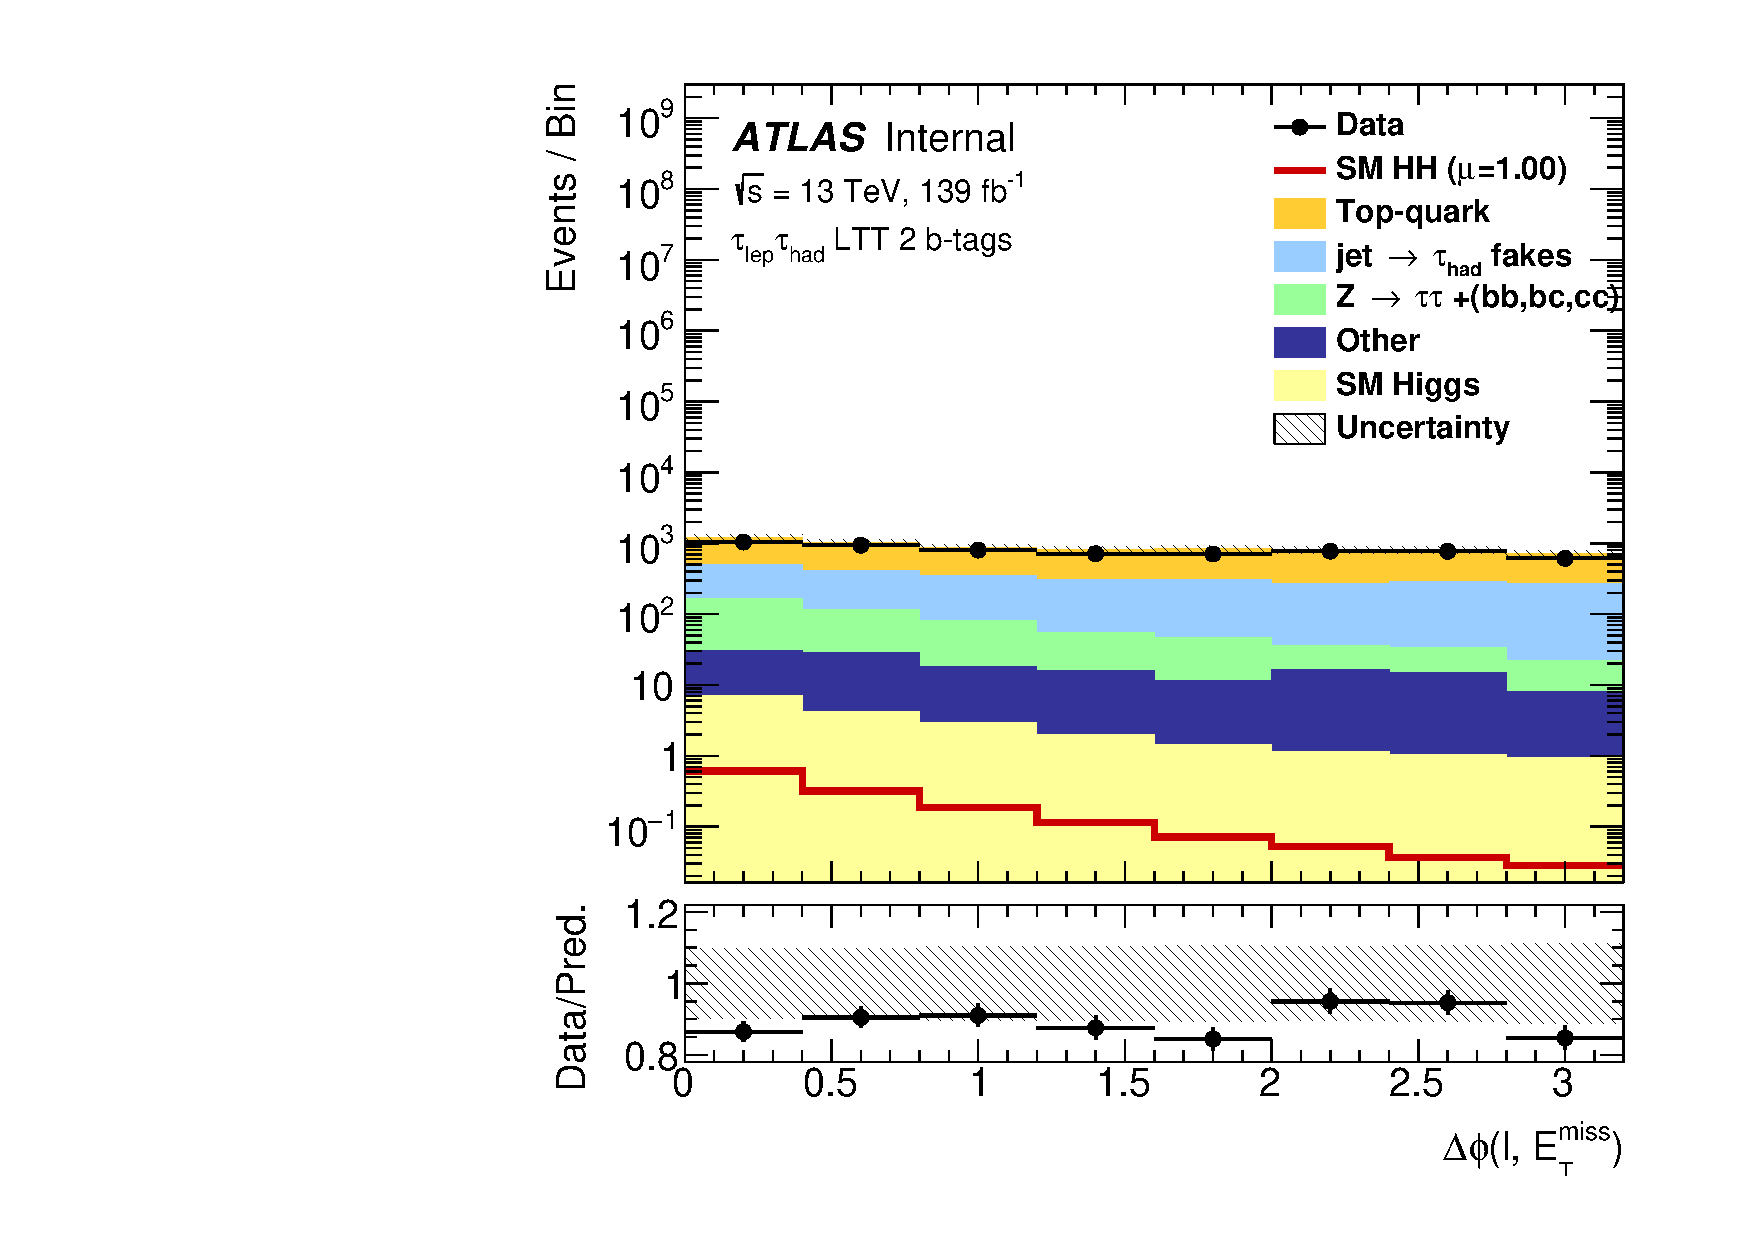
\includegraphics[width=.32\textwidth]{DiHiggs/plots/MVA/LTT/Region_BMin0_incJet1_distdPhiLep0MET_J2_D_T2_SpcTauLH_Y2015_LTT1_L1_Prefitlog.pdf} \\
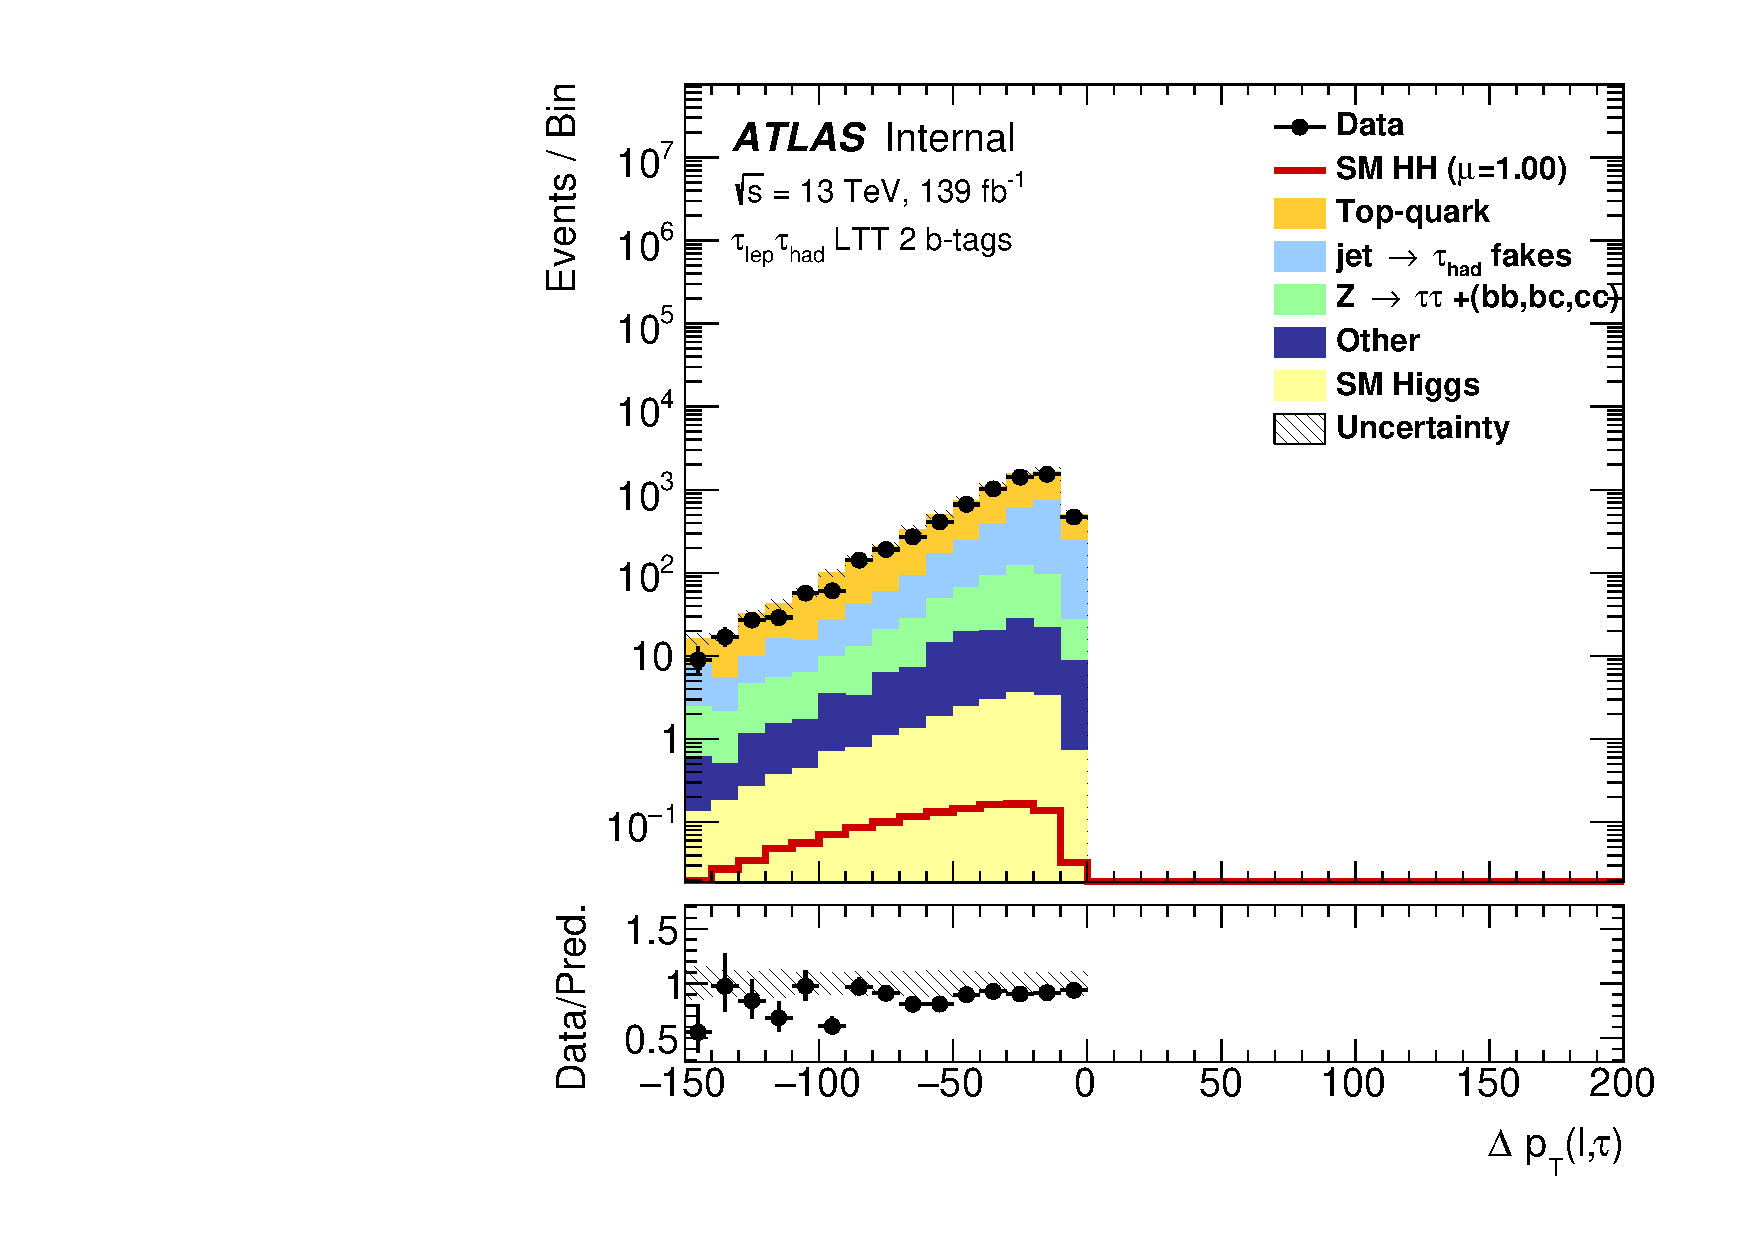
\includegraphics[width=.32\textwidth]{DiHiggs/plots/MVA/LTT/Region_BMin0_incJet1_distdPtLepTau_J2_D_T2_SpcTauLH_Y2015_LTT1_L1_Prefitlog.pdf}
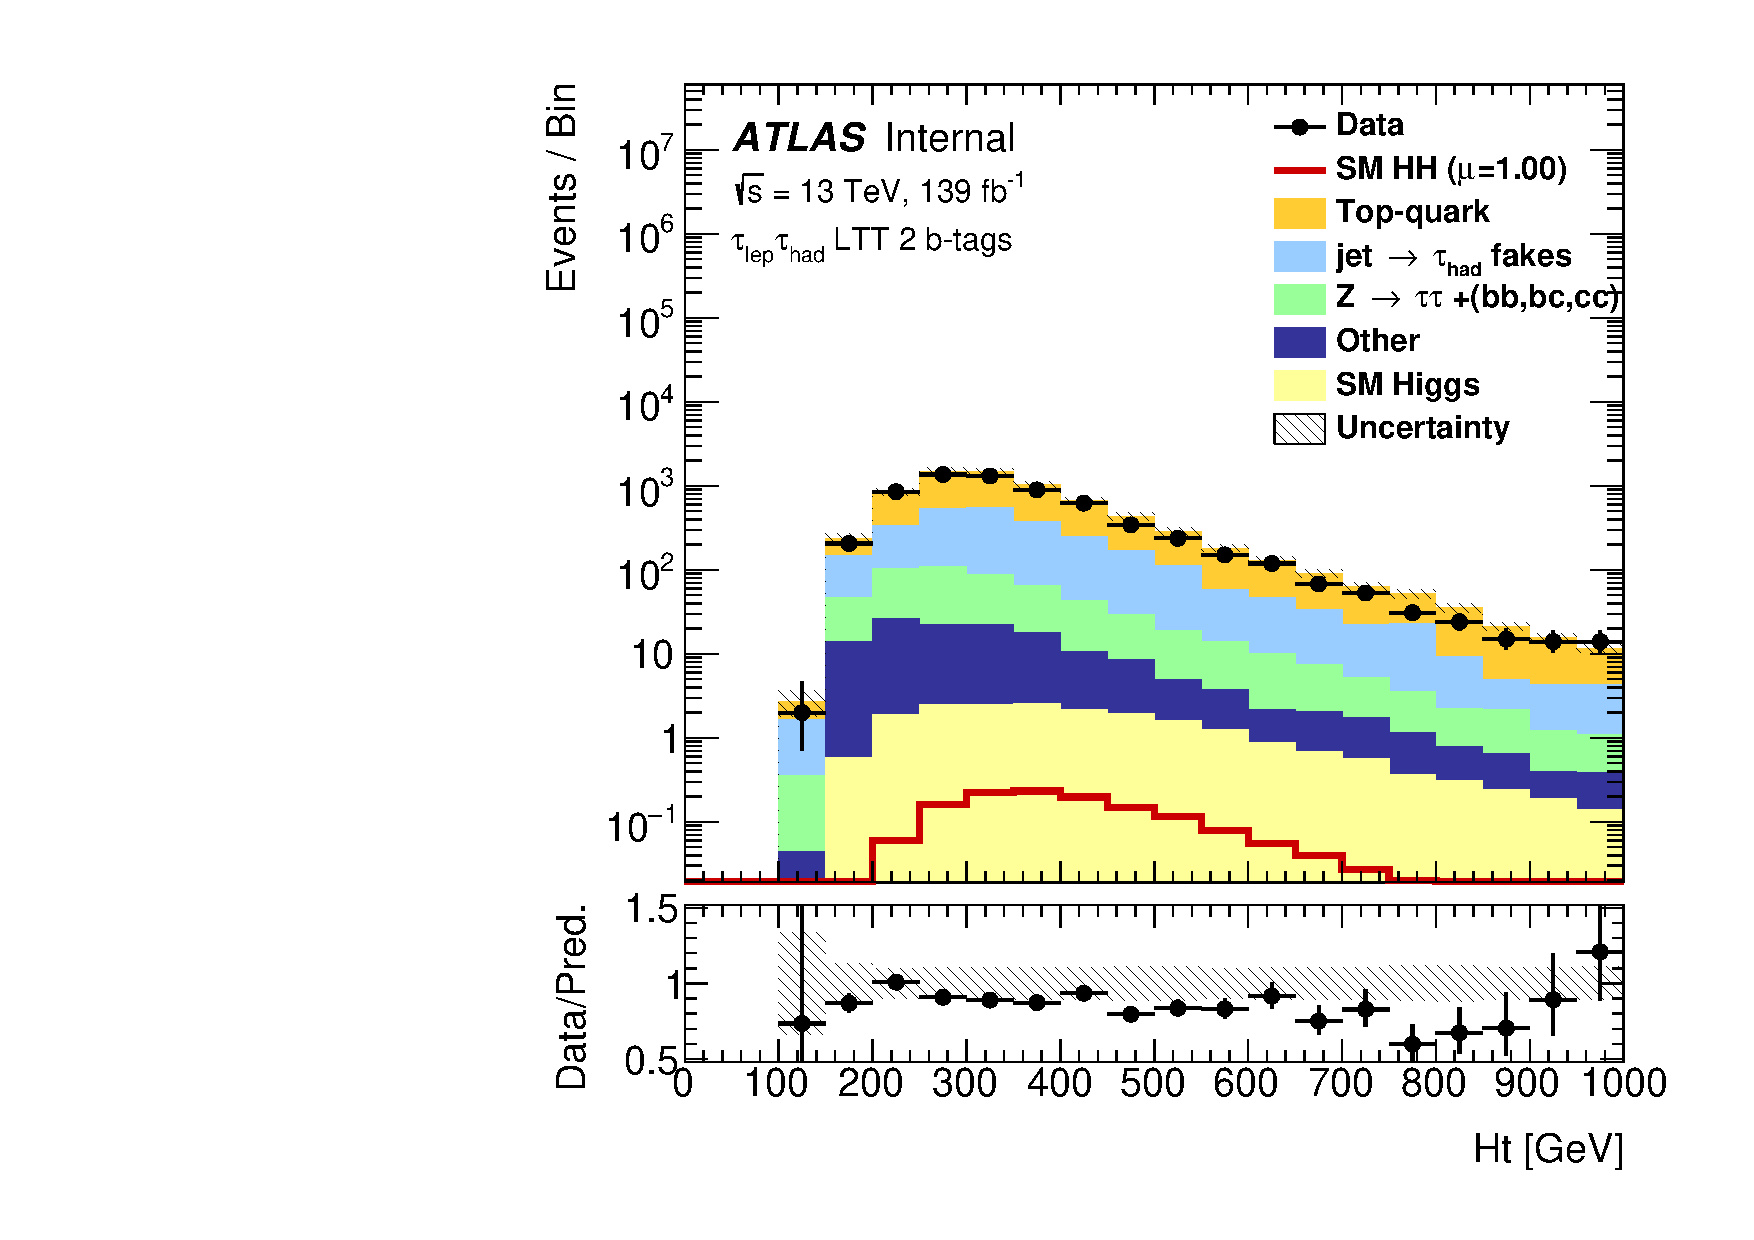
\includegraphics[width=.32\textwidth]{DiHiggs/plots/MVA/LTT/Region_BMin0_incJet1_distHt_J2_D_T2_SpcTauLH_Y2015_LTT1_L1_Prefitlog.pdf}
\caption{Pre-fit PNN/NN input variable distributions in the di-Higgs $bb\lephad$ LTT signal region.}
\label{fig:lephadmvainputsltt}
\end{figure}


\subsection{MVA hyper parameters optimisation and trainning}
Standardised variables are used for all NN trainings described in the following.
The input variables are standardised by subtracting the median and dividing by the
interquartile range.
During training, the sum of all backgrounds normalised to
their respective cross-sections is used. 
The neural networks are trained using
Keras~\cite{keras} and Tensorflow~\cite{tensorflow}.
The hyperparameters used for training the NN (PNN) are 
listed in Table~\ref{tab:parameters_NN_LepHad} (\ref{tab:parameters_PNN_LepHad}).
The rectified linear unit (ReLU) and sigmoidal activation fuunctions 
are used for the hidden layers and output layers respectively.
The loss function is the binary cross-entropy, 
using L2 regularisation (`Ridge regression', which adds squared amplitude 
for the penalty term), and the optimiser used 
is stochastic gradient descent~\cite{Goodfellow-et-al-2016}.
The numbers of epoch, batch size, learning rate and 
learning rate decay are again listed in the tables below. 
The Nesterov momentum is used in the gradient descent. 
These hyperparameters were optimised 
separately for each MVA by a Bayesian optimisation procedure with 
a Gaussian process. 
A metric for the NN hyperparameters optimisation is defined 
as the quadrature sum of approximated significances
of bins with at least 5 expected background events,
while for the PNN, a metric is defined as the approximated
significance after an optimised cut (a cut that maximises the 
significance), and the bins after cut are required to have 
at least 5 expected background events. 
The metric is evaluated on the validation and testing sets,
and the hyper parameters giving the best value are chosen. 
The NN and PNN are retrained when the optimisation is done. 

% The hyperparameters were optimised separately for each MVA 
% using a random scan followed by a Bayesian optimisation procedure. 
% % The 375~GeV resonant $HH$ signal is not used in the PNN trainings. 
% In the case of the PNNs the signal masses were averaged 
% by weighting by the mass space nearest the chosen sample,
% to represent all parts of the mass space equally.
% The network is retrained once the optimisation is done 
% to avoid bias due to overlapping the training and testing sets. % or valdiation and test sets? 
% There is also pseudo-randomness in the network training 
% procedure which results in the trained network having multiple 
% possible sets of network weights and biases even without a change in the input dataset. 
% The weights and biases of these MVAs have also been 
% explicitly compared between the first training which occurred 
% during hyperparameter optimisation, and the second training which 
% is used in the analysis, and they can be seen to have changed.
% Despite the above reasoning making it unlikely that any bias can result 
% from the overlapping training and testing sets, this is tested explicitly as described below.
% A nested cross-validation was also considered to ensure that 
% there was no bias from the overlapping validation and 
% testing datasets, however, the large $\tau_\text{lep}\tau_\text{had}$ 
% samples sizes mean that this would have compromised the number of hyperparameter sets 
% which could be trialled, and multiple MVAs would have been needed for each analysis category. In order to check that this approach did not introduce a significant 
% bias, the full nested optimisation was performed in the non-resonant LTT search category, and the stat-only limits with no data-driven fakes were compared. The 
% limit was found to deteriorate by just 0.6\% (1.7\%) with(out) retraining on the whole inner-fold from the nested cross validation. Similar studies were also performed 
% in the non-resonant $\tau_\text{had}\tau_\text{had}$ category, and the differences in the estimated significance (as per the optimisation metric) was found to be on 
% the level of 2.4\%.
% Dropout regularisation was also tried, but were found to provide no improvements. The lower mass samples, where the $bb\tau_\mathrm{lep}\tau_\mathrm{had}$ 
% channels are expected to provide most sensitivity, were given increased weights to see if this improved performance for these signal hypotheses, but no gains were 
% observed, so this was not adopted.
% Studies on the performance of the MVAs are reported in Appendix~\ref{sec:appendix_pnn_HH}.

\begin{table}
  \centering
  \small
  \begin{tabular}{|c|c|c|}
    \hline
    Parameter & Value for SLT & Value for LTT\\
    \hline
    Layer sizes & 512 512 & 512 512 512\\
    Epochs & 241 & 238\\
    Batch-size & 34 & 35\\
    Learning rate & 0.500 & 0.500\\
    Learning rate decay & 4.15$\times 10^{-3}$ & 4.20$\times 10^{-3}$\\
    Nesterov momentum & 0.944 & 0.791\\
    L2 regularisation weight & 1.00$\times 10^{-5}$ & 1.65$\times 10^{-5}$\\
    \hline
  \end{tabular}
  \caption{Training parameters used for the di-Higgs \lephad non-resonant NNs.
  Table reproduced from Ref.~\cite{dihiggs-conf}.}
  \label{tab:parameters_NN_LepHad}
\end{table}

\begin{table}
  \centering
  \small
  \begin{tabular}{|c|c|c|}
    \hline
    Parameter & Value for SLT & Value for LTT\\
    \hline
    Layer sizes & 512 512 & 256 256 256\\
    Epochs & 245 & 296\\
    Batch-size & 33 & 24\\
    Learning rate & 0.500 & 0.377\\
    Learning rate decay & 4.55$\times 10^{-3}$ & 3.38$\times 10^{-3}$\\
    Nesterov momentum & 0.975 & 0.975\\
    L2 regularisation weight & 5.45$\times 10^{-7}$ & 8.64$\times 10^{-6}$\\
    \hline
  \end{tabular}
  \caption{Training parameters used for the di-Higgs \lephad resonant PNNs.
  Table reproduced from Ref.~\cite{dihiggs-conf}.}
  \label{tab:parameters_PNN_LepHad}
\end{table}


During training for the NN (PNNs), the two-fold validation is used. 
The data set is partitioned into two sets depending on 
the event numbers being even or odd, where one set is used for
training with the other set being used for validation, vice versa.
To check if the neural networks are overtrained, 
the loss functions as a function of the training epoch for 
the NN (PNNs) are shown in Figure~\ref{fig:overtrainingtestnn} 
(Figure~\ref{fig:overtrainingtestpnn}) for the 
SLT and LTT channels. A stable generalisation gap is seen between 
the training and validation, indicating that the overtraining is small
Further checks are done using a much simpler architecture consisting of three layers
of 32 nodes for the LTT channel. A large gap is still seen, indicating the
generalisation gap is due to limited data rather than effective capacity of
the neural networks.
Additional plots of the NN (PNNs) output distribution of the signal and summed background
can be found in Appendix~\ref{sec:appendix:mva}, 
Figure~\ref{sec:appendix:overfittingtestSLT} and Figure~\ref{fig:overfittingtestLTT}
for the SLT and LTT channel, respectively. 

\begin{figure}
  \centering
  \subfloat[]{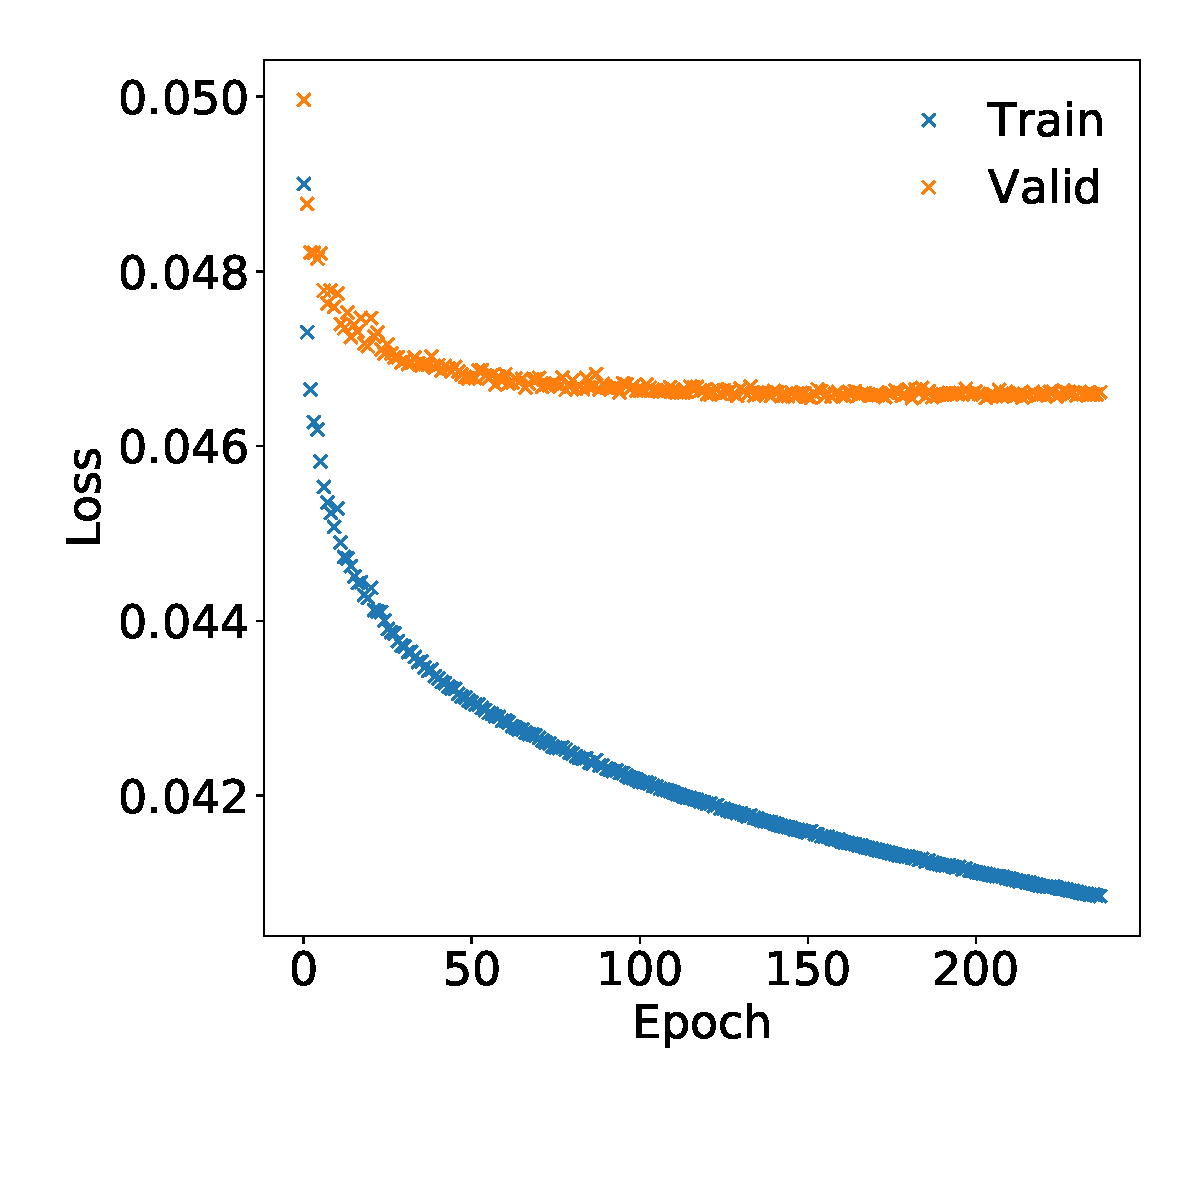
\includegraphics[width=.45\textwidth]{DiHiggs/plots/MVA/Validation/OvertrainingPlotNNLTT.pdf}}\quad
  \subfloat[]{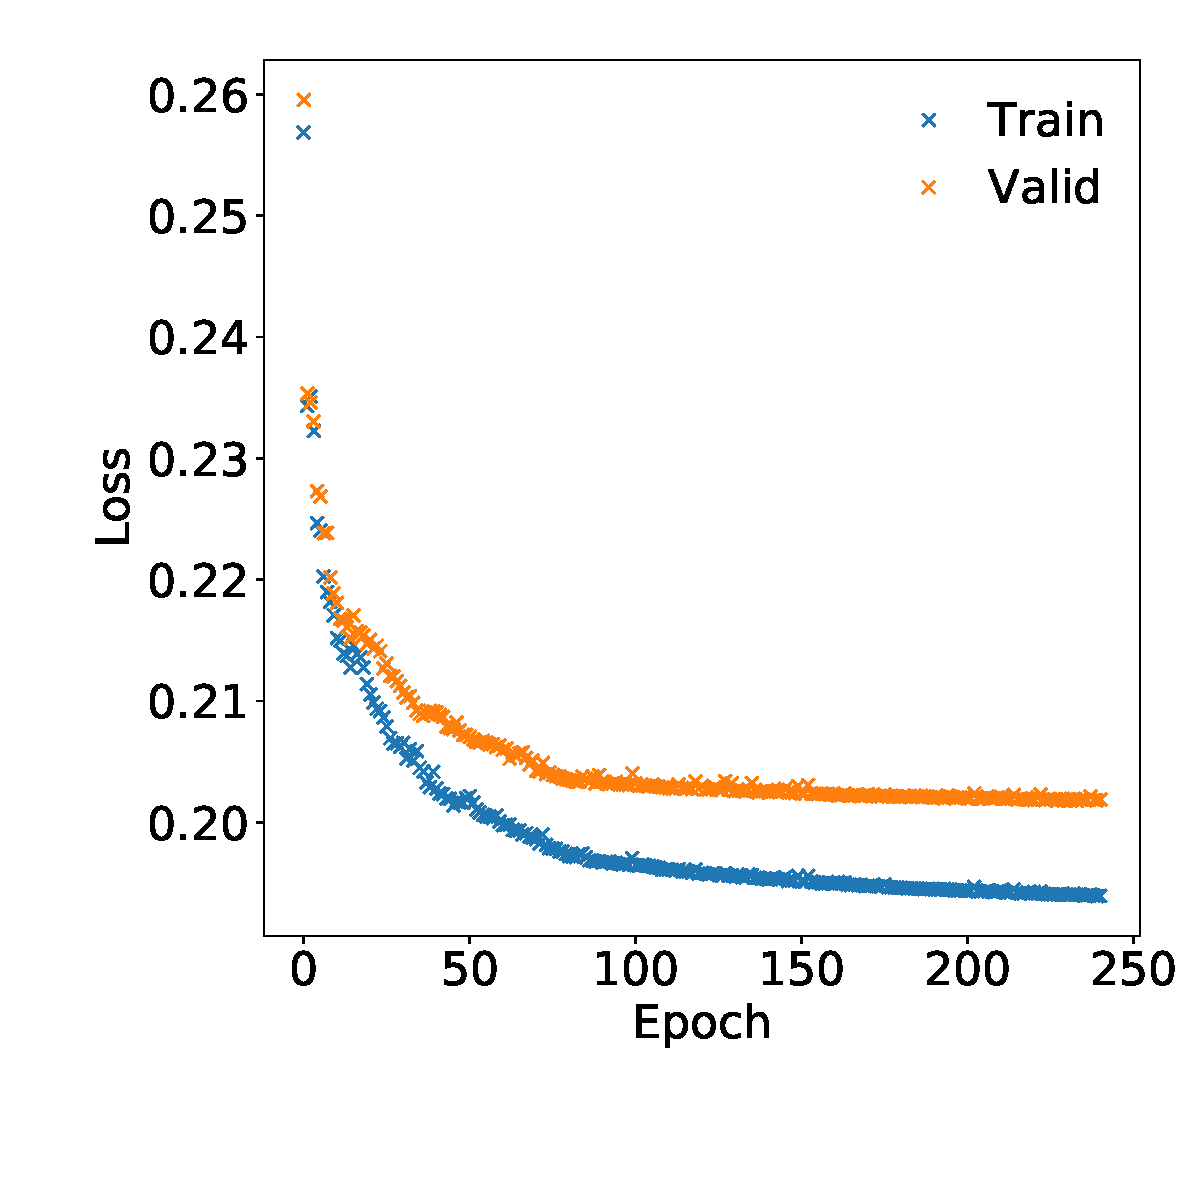
\includegraphics[width=.45\textwidth]{DiHiggs/plots/MVA/Validation/OvertrainingPlotNNSLT.pdf}}\quad
  \caption{Non-resonant NN loss functions as a function of training epochs evaluated 
  using the two-fold cross validation, for the (a) LTT and (b) SLT categories. 
  Figures reproduced from analysis internal notes. 
  }
  \label{fig:overtrainingtestnn}
\end{figure}

\begin{figure}
  \centering
  \subfloat[]{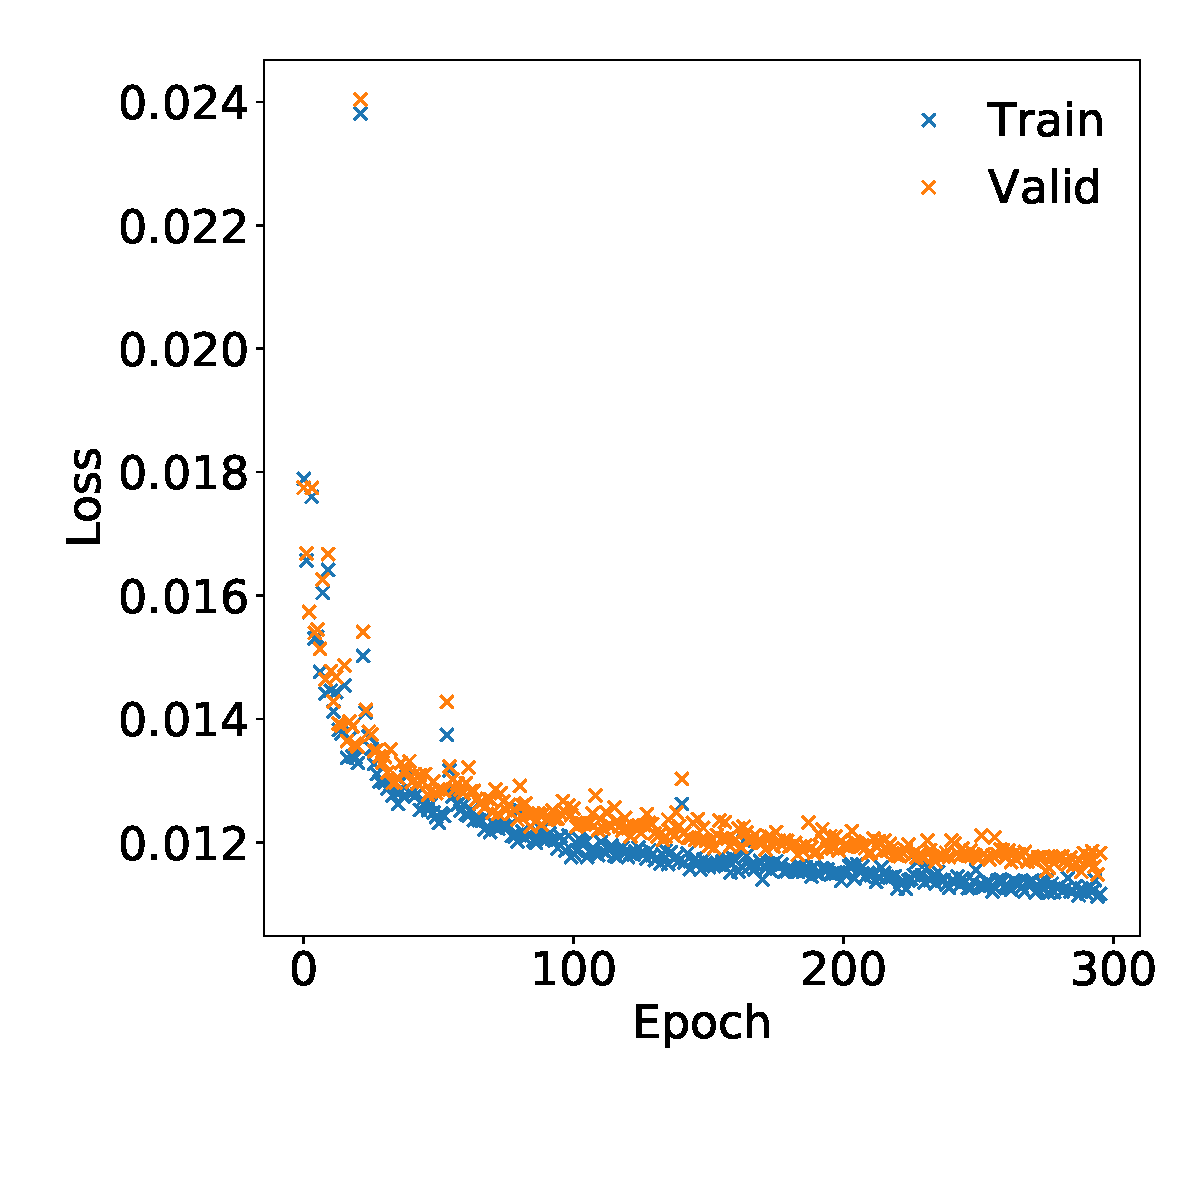
\includegraphics[width=.45\textwidth]{DiHiggs/plots/MVA/Validation/OvertrainingPlotLTT.pdf}}\quad
  \subfloat[]{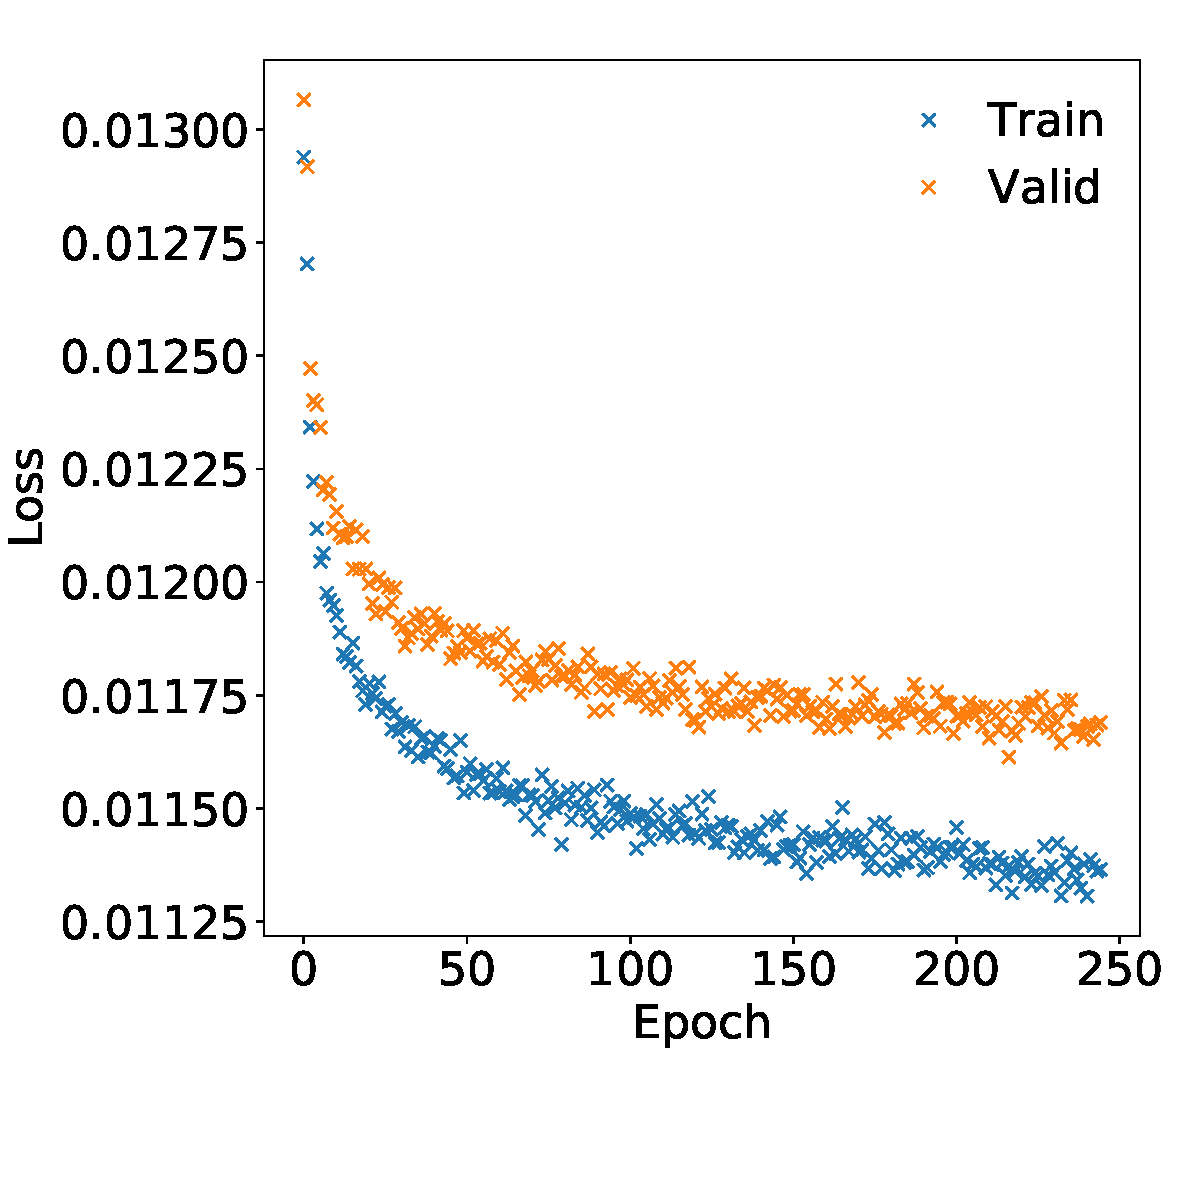
\includegraphics[width=.45\textwidth]{DiHiggs/plots/MVA/Validation/OvertrainingPlotSLT.pdf}}\quad
  \caption{PNN loss functions as a function of training epochs evaluated 
  using the two-fold cross validation, for the (a) LTT and (b) SLT categories.
  Figures reproduced from analysis internal notes. }
  \label{fig:overtrainingtestpnn}
\end{figure}



In addition, the PNNs are trained on all the signals simultaneously, 
and are parameterised by the mass of the resonance $HH$ sample. 
Since the background does not have a well-defined value of the
resonance mass, the background events are assigned a random value
generated from the signal mass parameter during training. 
The PNNs therefore provide near-optimal sensitivity over the
range of signal masses considered. 
Additionally, the PNNs interpolate well between the mass points used for the training.
This is checked by plotting the PNN response in terms of Asimov significance
as a function of the PNN mass parameter, which is shown in Figure~\ref{fig:MVA:mass-response}. 
The PNNs show very high significance over whole scanning mass spectrum. 
The minimum significance appears in the vicinity of low signal masses, reaching a 
value of 0.7. As the signal mass increases, the `gap' becomes smaller and smaller.



\begin{figure}[htbp]
\centering
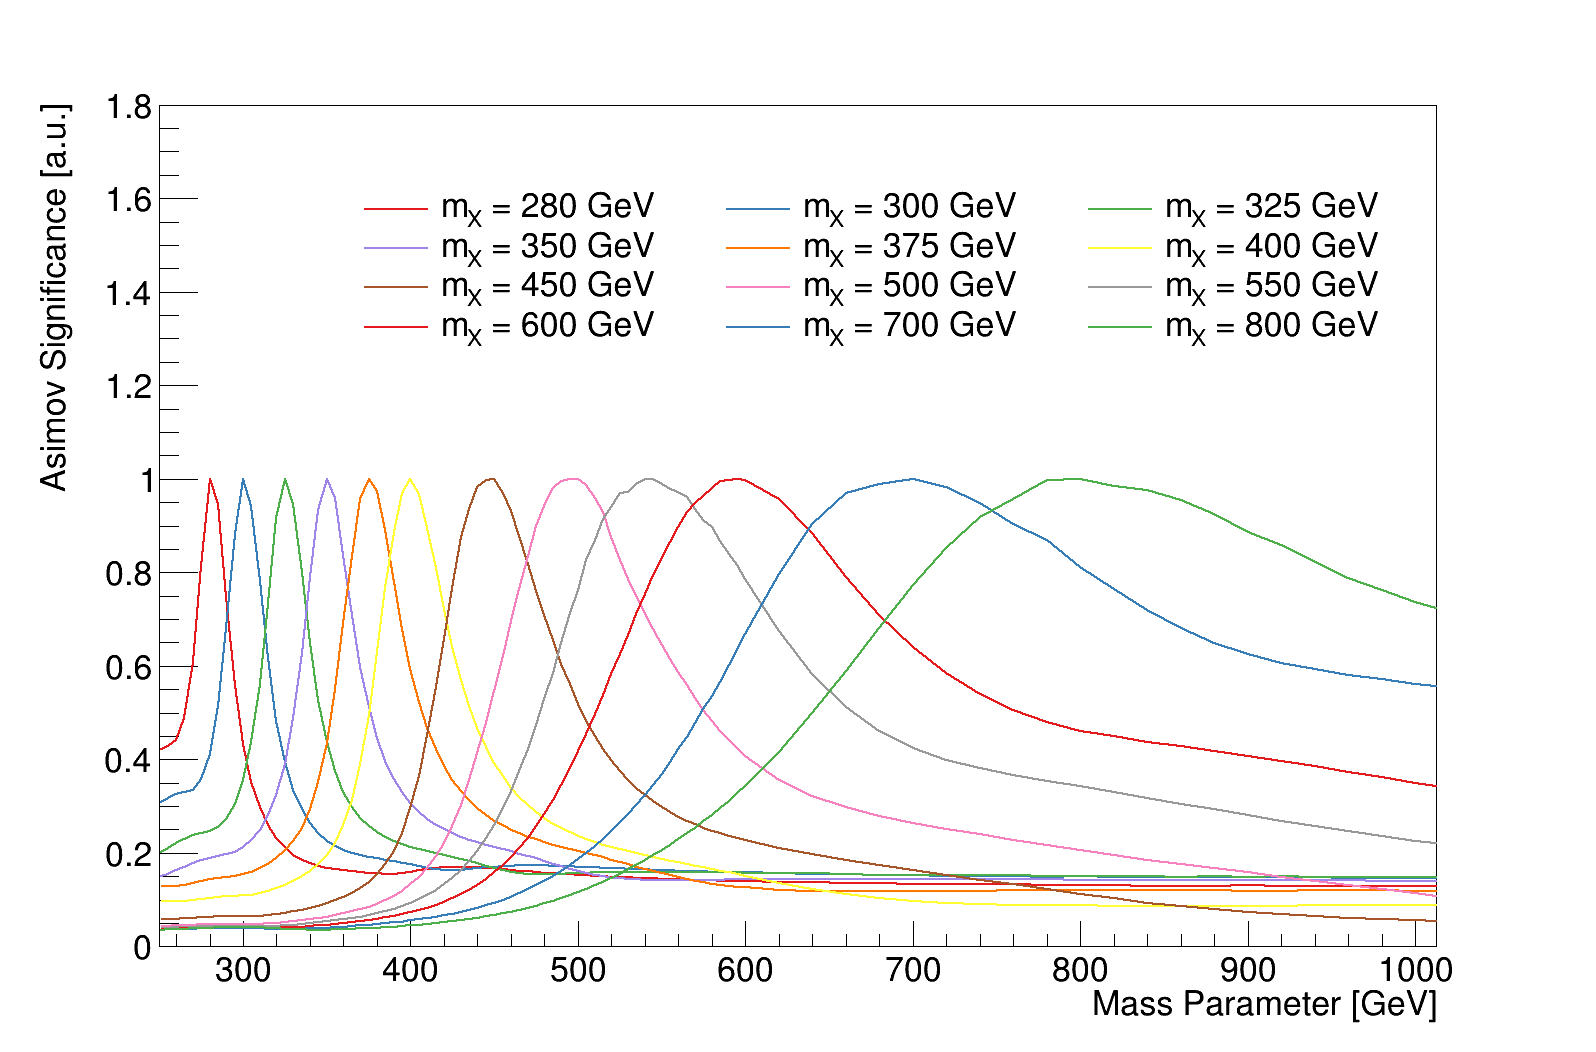
\includegraphics[width=0.85\linewidth]{DiHiggs/plots/mass_response.png}
% location /hepstore/zhiyuan/Code_latest/run_Asimov/parametricnet/scripts/plots, run  python plot_mass.py to get
\caption{
    PNN response in terms of Asimov significance as a function of the PNN mass parameter obtained for
signal samples with different masses. Due to a large difference in acceptance times
efficiency of the \lephad\ channel signal region selection depending on the mass of the resonance, 
all significances are scaled so that the maximum significance is 1 for better visibility.}
\label{fig:MVA:mass-response}
\end{figure}



\subsection{MVA output distributions}
Finally, the output distributions of the NN and the PNNs are shown in 
Figure~\ref{fig:lephadmvaoutput}. 
The data distributions are not blinded here as the definition of the event
pre-selection is very loose. 
To validate the MC modelling, the pre-fit PNN score distributions are shown in 
Figure~\ref{fig:lephadmvaCRoutput} in Appendix~\ref{sec:appendix:mva} in the 1-tag control region. 
The binning of the MVA output discriminant will be defined in sectioin~\ref{} TODO:
ref to fit section. 
The events yields in the last three bins of the MVA discriminant are shown in 
Table~\ref{tab:yields_LastMVABin_LepHad_SLT} (Table~\ref{tab:yields_LastMVABin_LepHad_LTT}) 
in Appendix~\ref{sec:appendix:mva} for SLT (LTT) channel, which are the most significant bins
for signal extraction. 



\begin{figure}
\centering
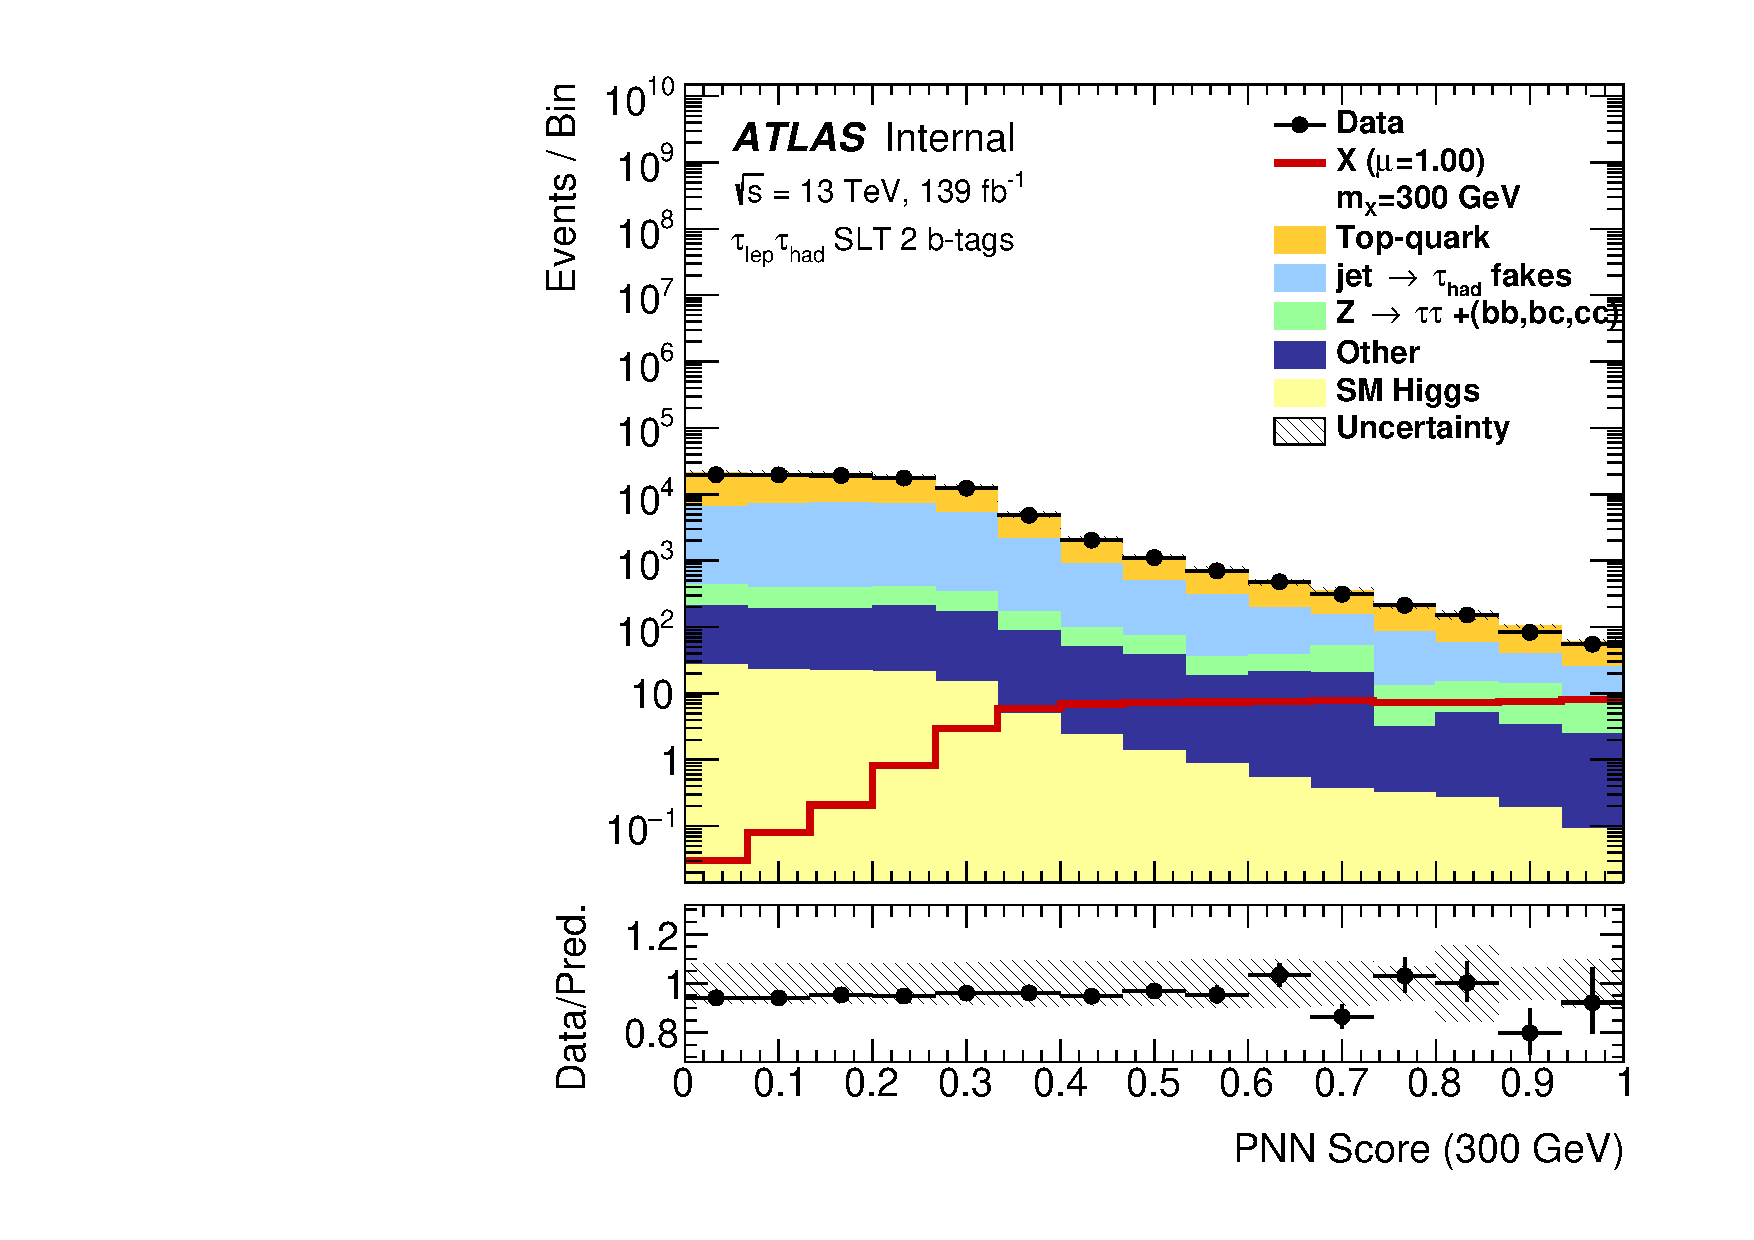
\includegraphics[width=.32\textwidth]{diHiggs/plots/MVA/SLT/Region_BMin0_incJet1_dist300_J2_D2HDMPNN_T2_SpcTauLH_Y2015_LTT0_L1_Prefitlog.pdf}
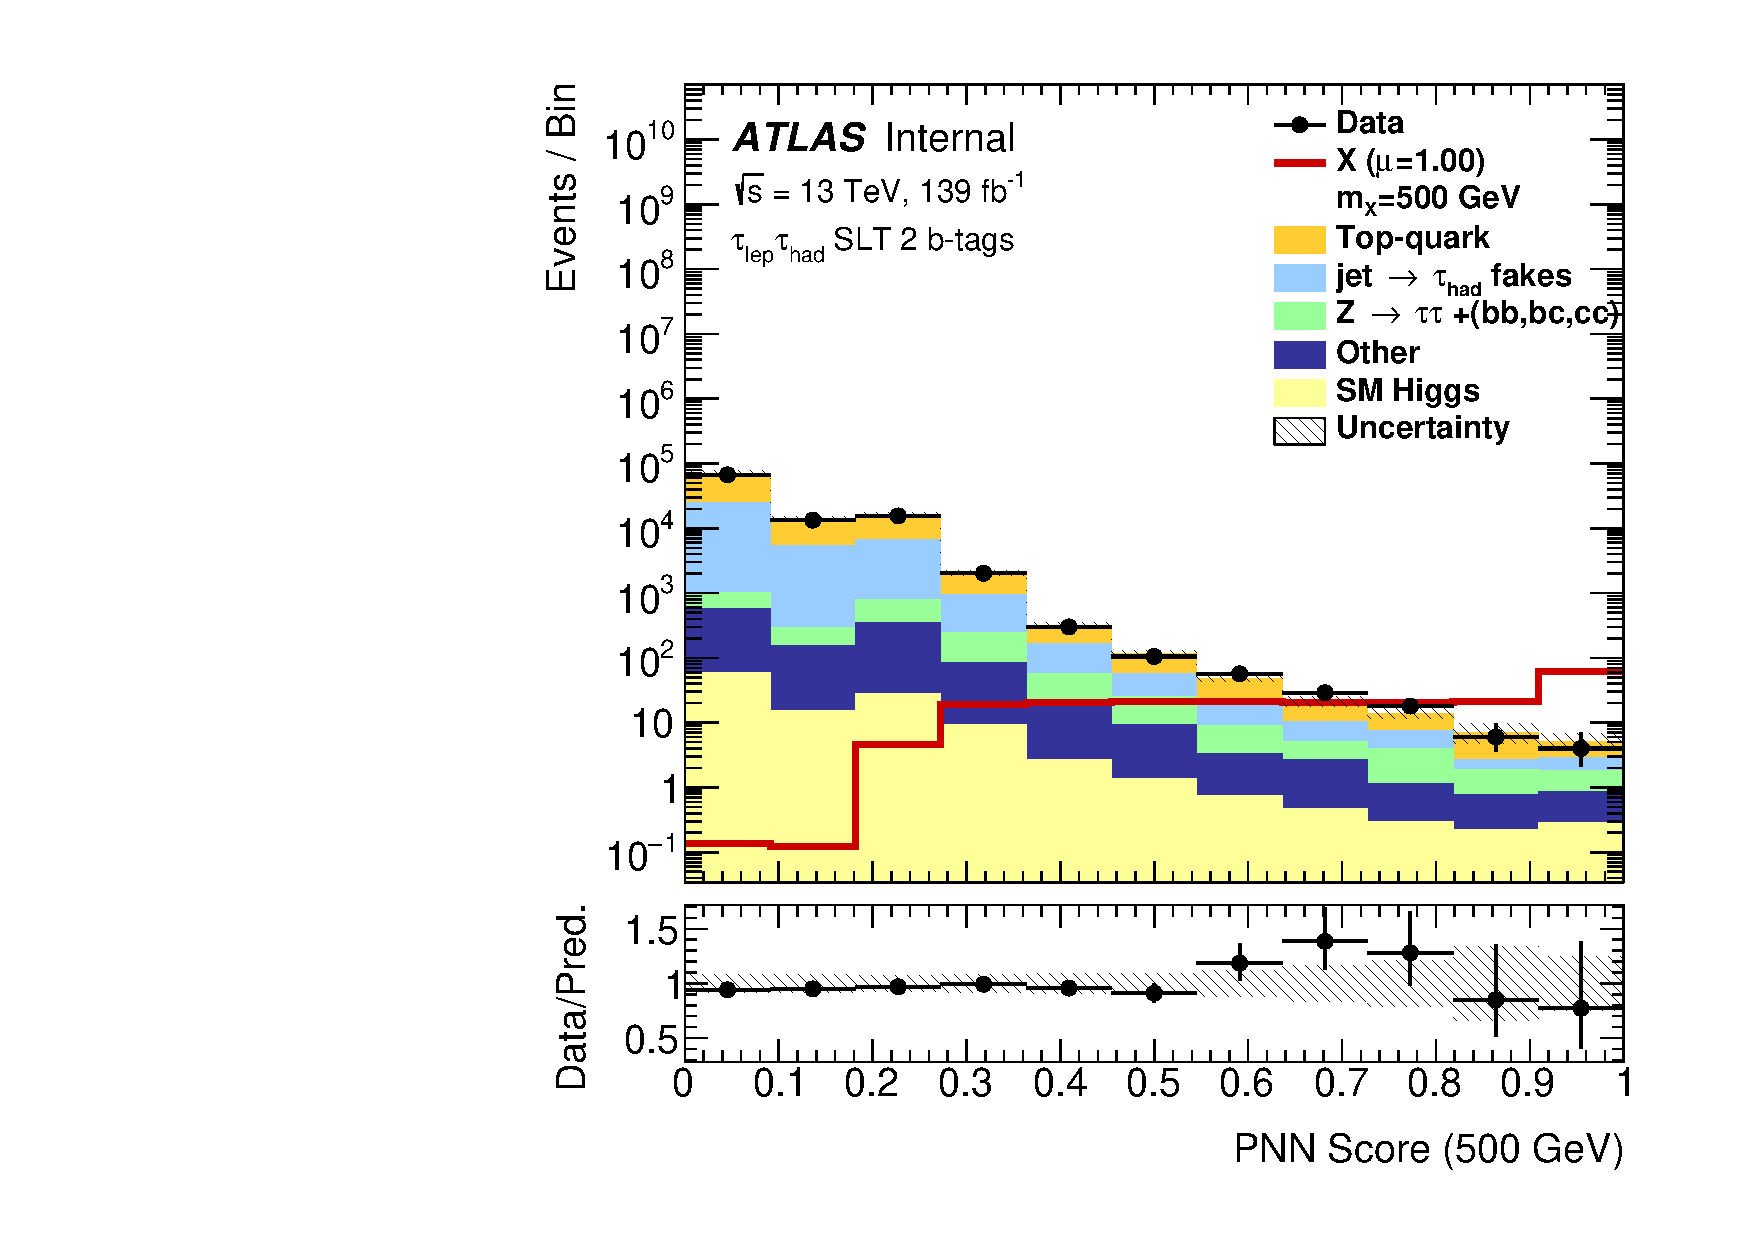
\includegraphics[width=.32\textwidth]{diHiggs/plots/MVA/SLT/Region_BMin0_incJet1_dist500_J2_D2HDMPNN_T2_SpcTauLH_Y2015_LTT0_L1_Prefitlog.pdf}
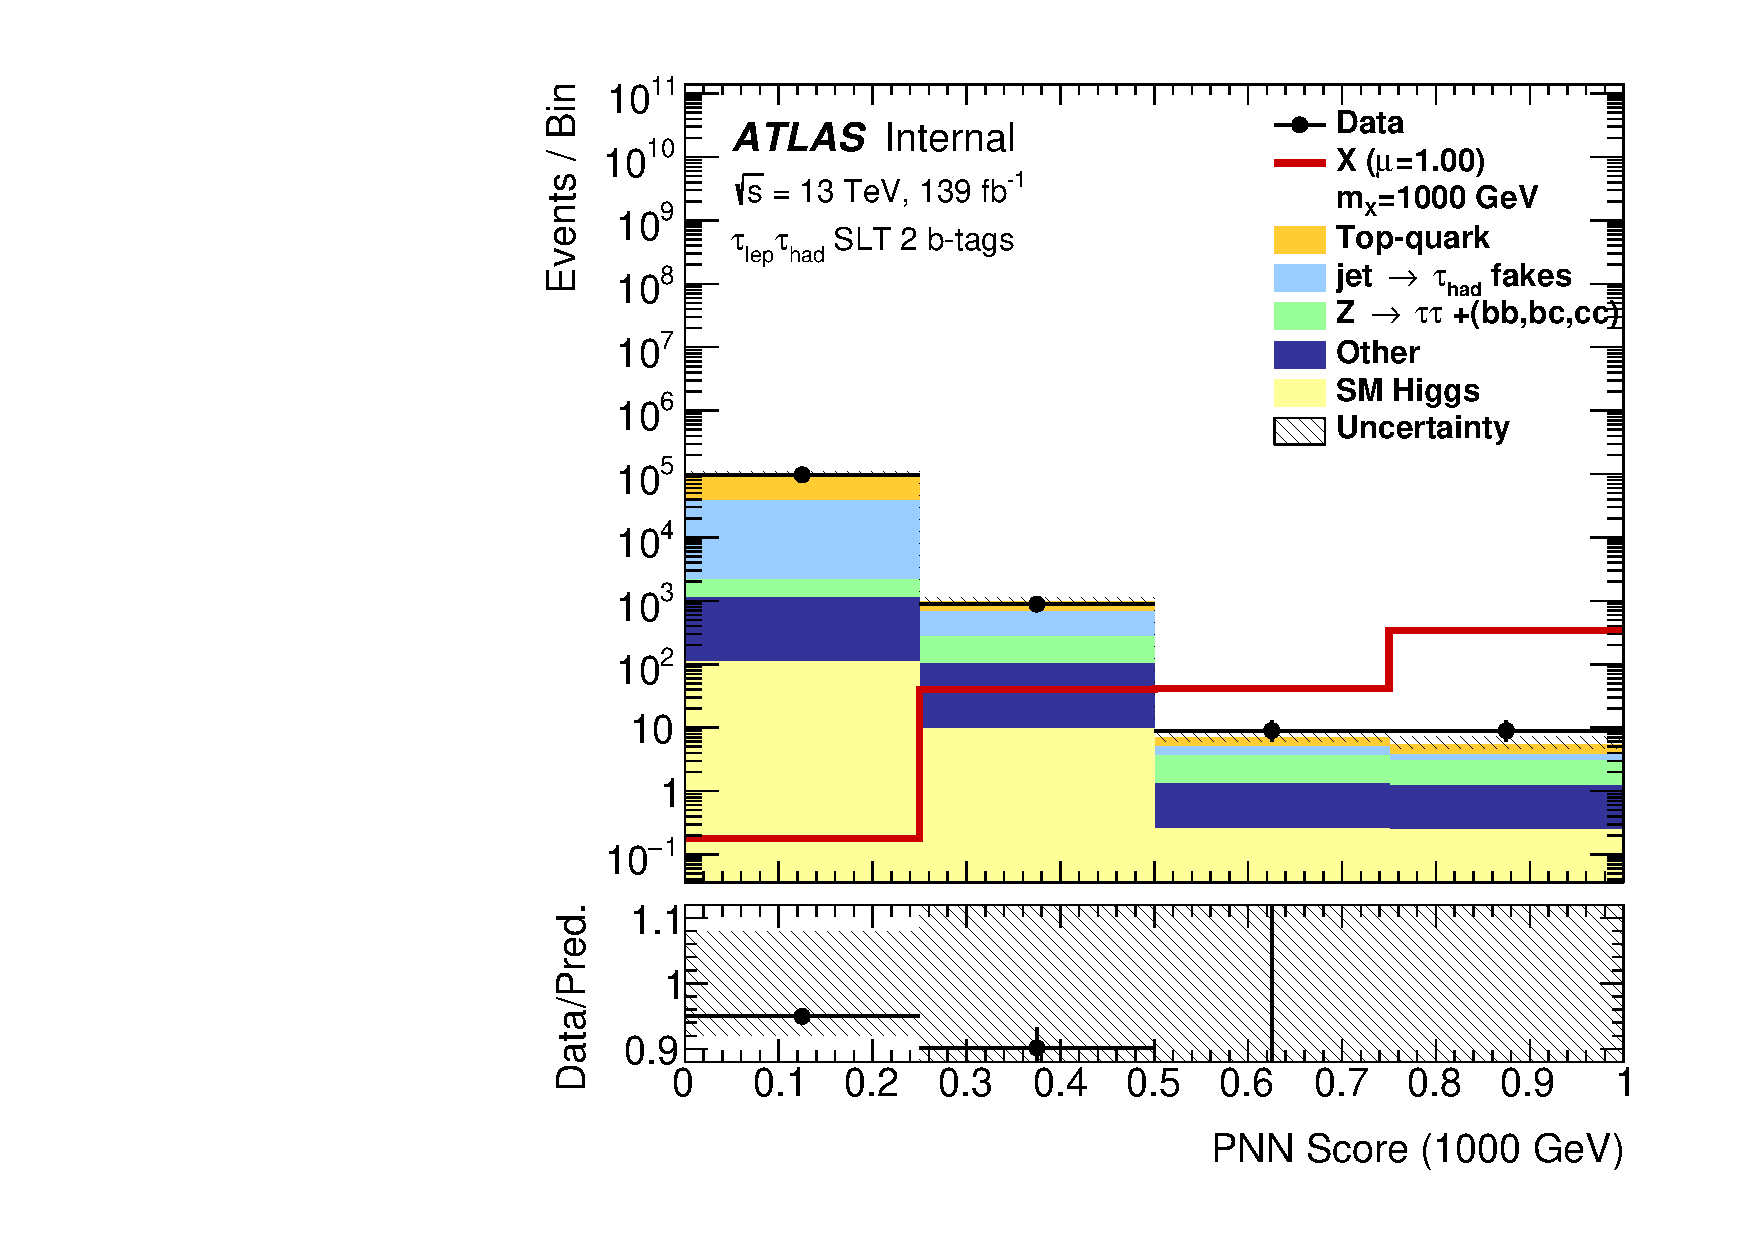
\includegraphics[width=.32\textwidth]{diHiggs/plots/MVA/SLT/Region_BMin0_incJet1_dist1000_J2_D2HDMPNN_T2_SpcTauLH_Y2015_LTT0_L1_Prefitlog.pdf} \\
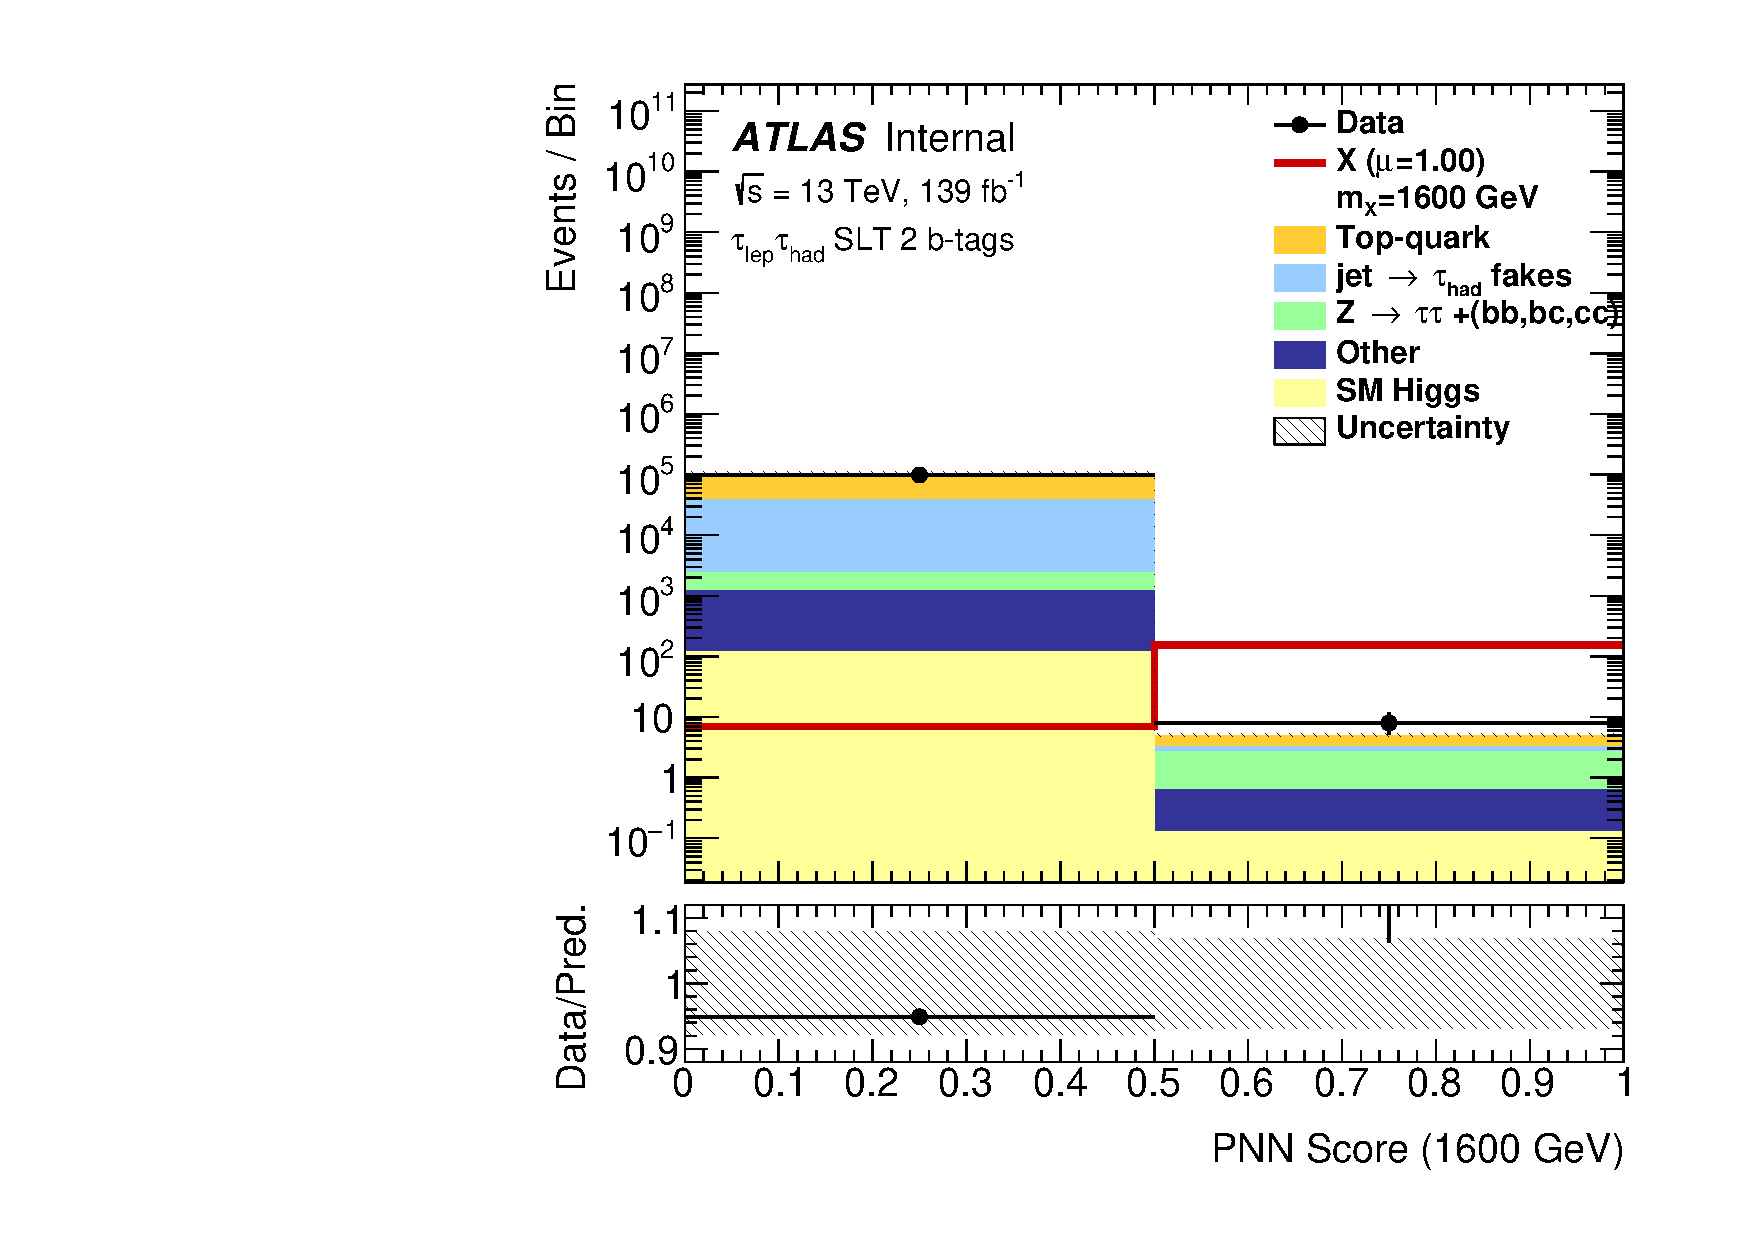
\includegraphics[width=.32\textwidth]{diHiggs/plots/MVA/SLT/Region_BMin0_incJet1_dist1600_J2_D2HDMPNN_T2_SpcTauLH_Y2015_LTT0_L1_Prefitlog.pdf} 
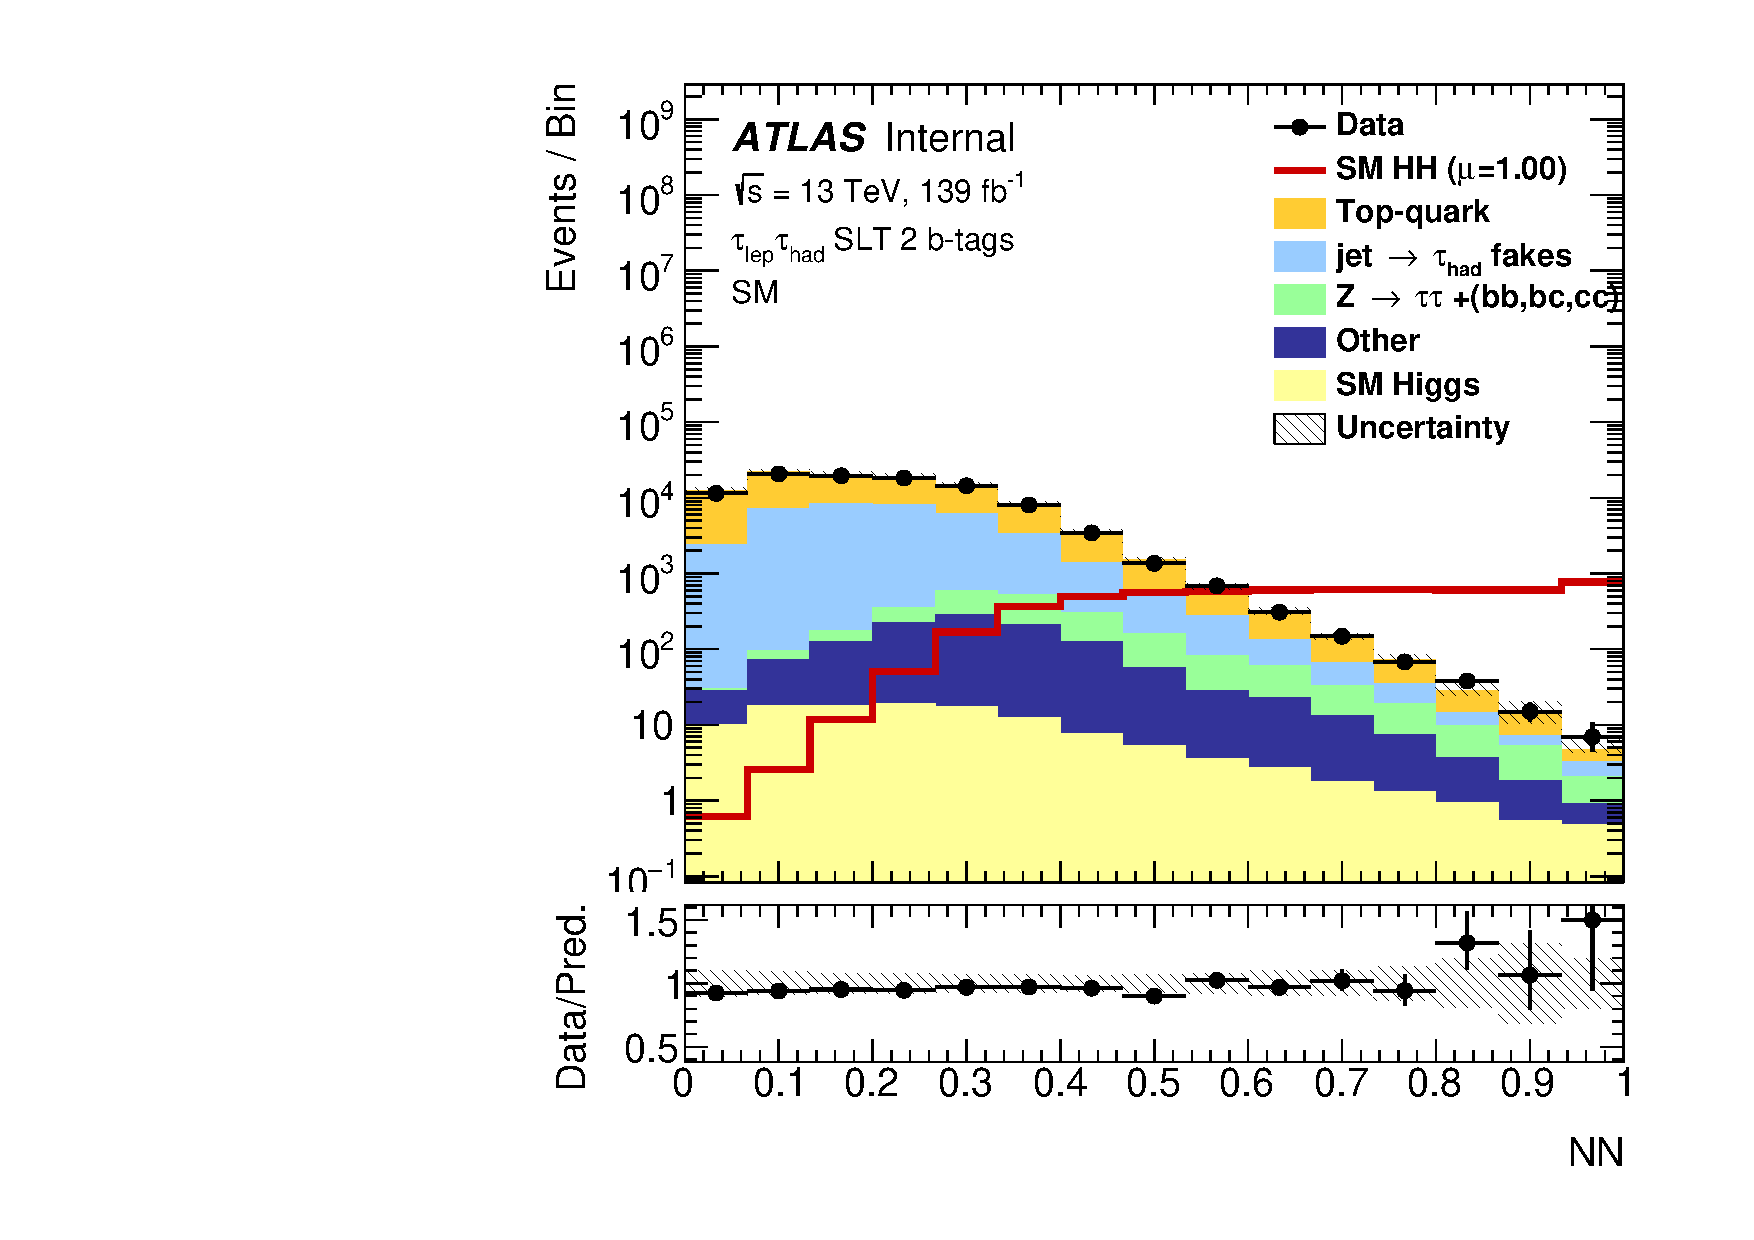
\includegraphics[width=.32\textwidth]{diHiggs/plots/MVA/SLT/Region_BMin0_incJet1_distNN_J2_DSM_T2_SpcTauLH_Y2015_LTT0_L1_Prefitlog.pdf} \\
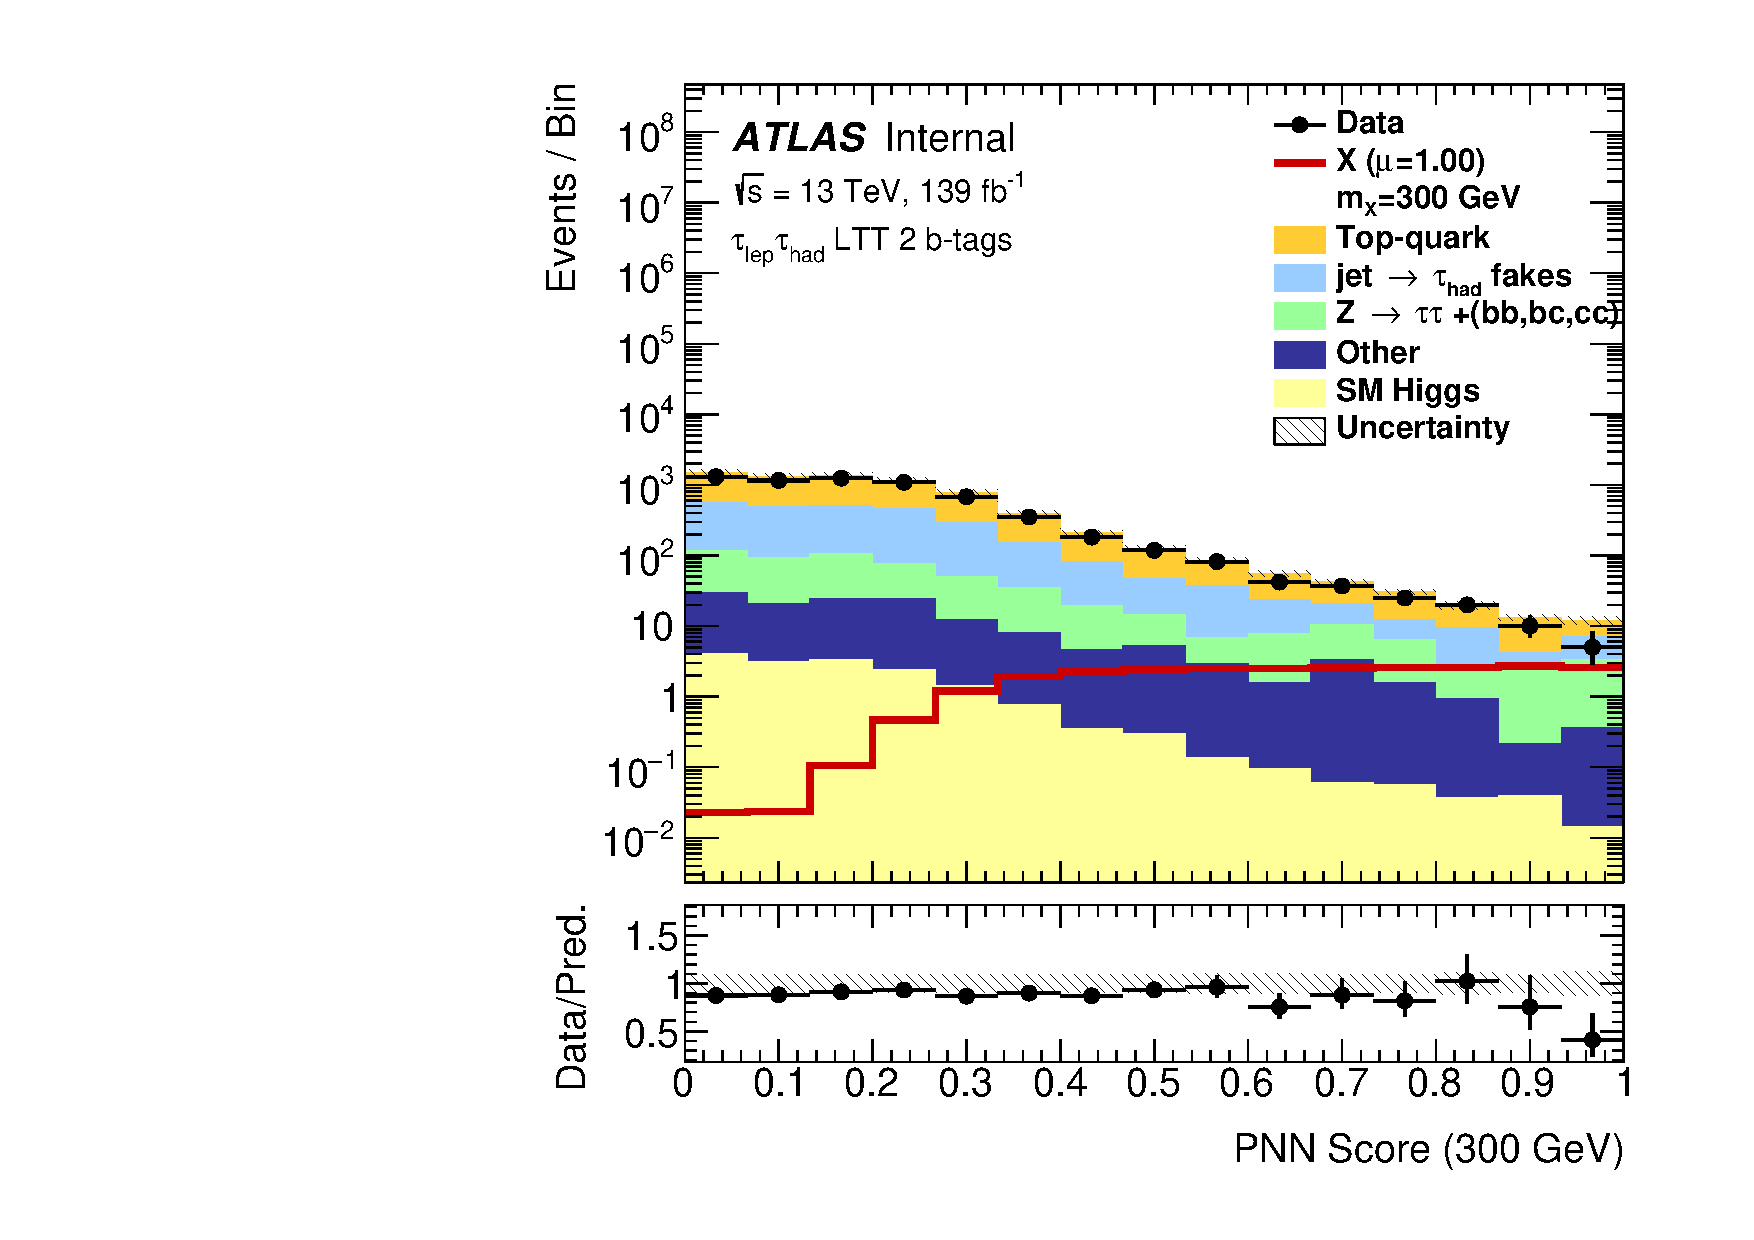
\includegraphics[width=.32\textwidth]{diHiggs/plots/MVA/LTT/Region_BMin0_incJet1_dist300_J2_D2HDMPNN_T2_SpcTauLH_Y2015_LTT1_L1_Prefitlog.pdf}
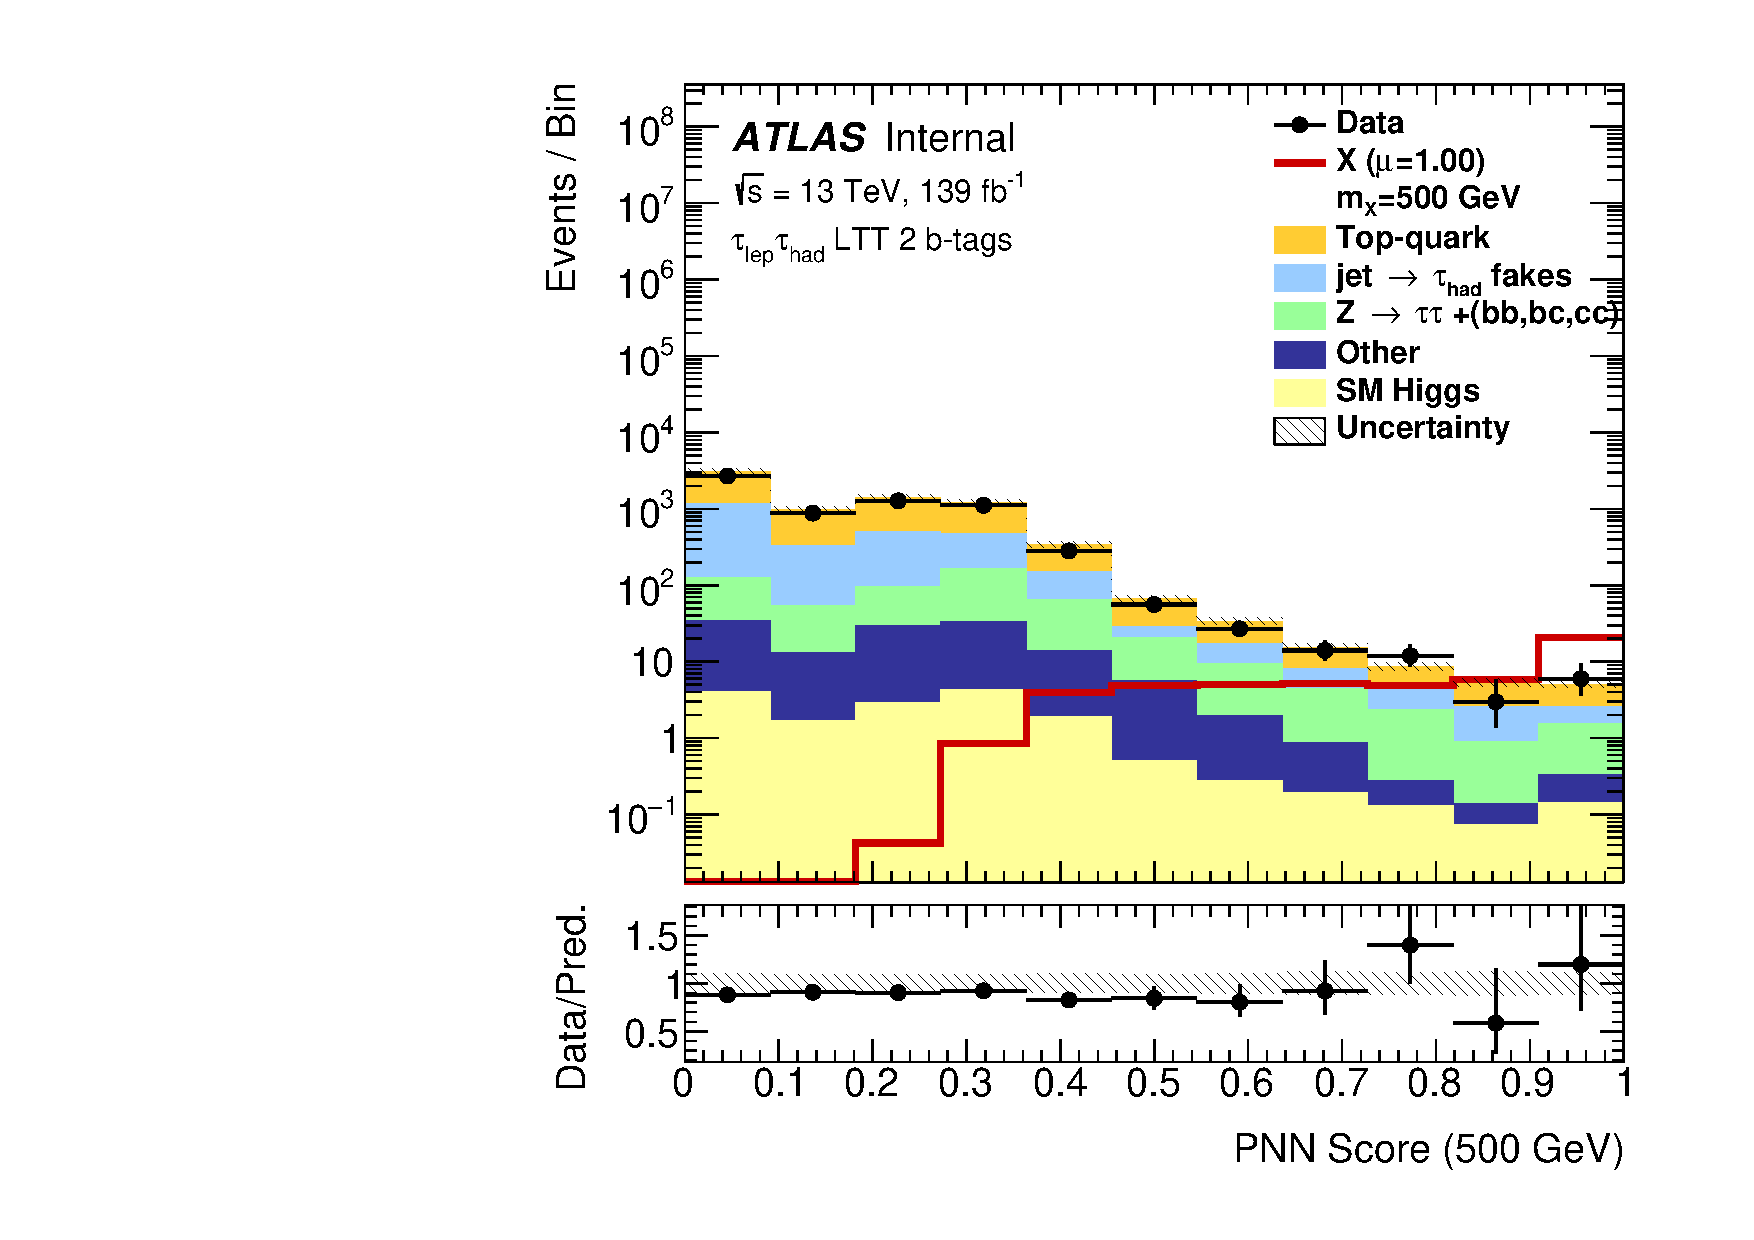
\includegraphics[width=.32\textwidth]{diHiggs/plots/MVA/LTT/Region_BMin0_incJet1_dist500_J2_D2HDMPNN_T2_SpcTauLH_Y2015_LTT1_L1_Prefitlog.pdf}
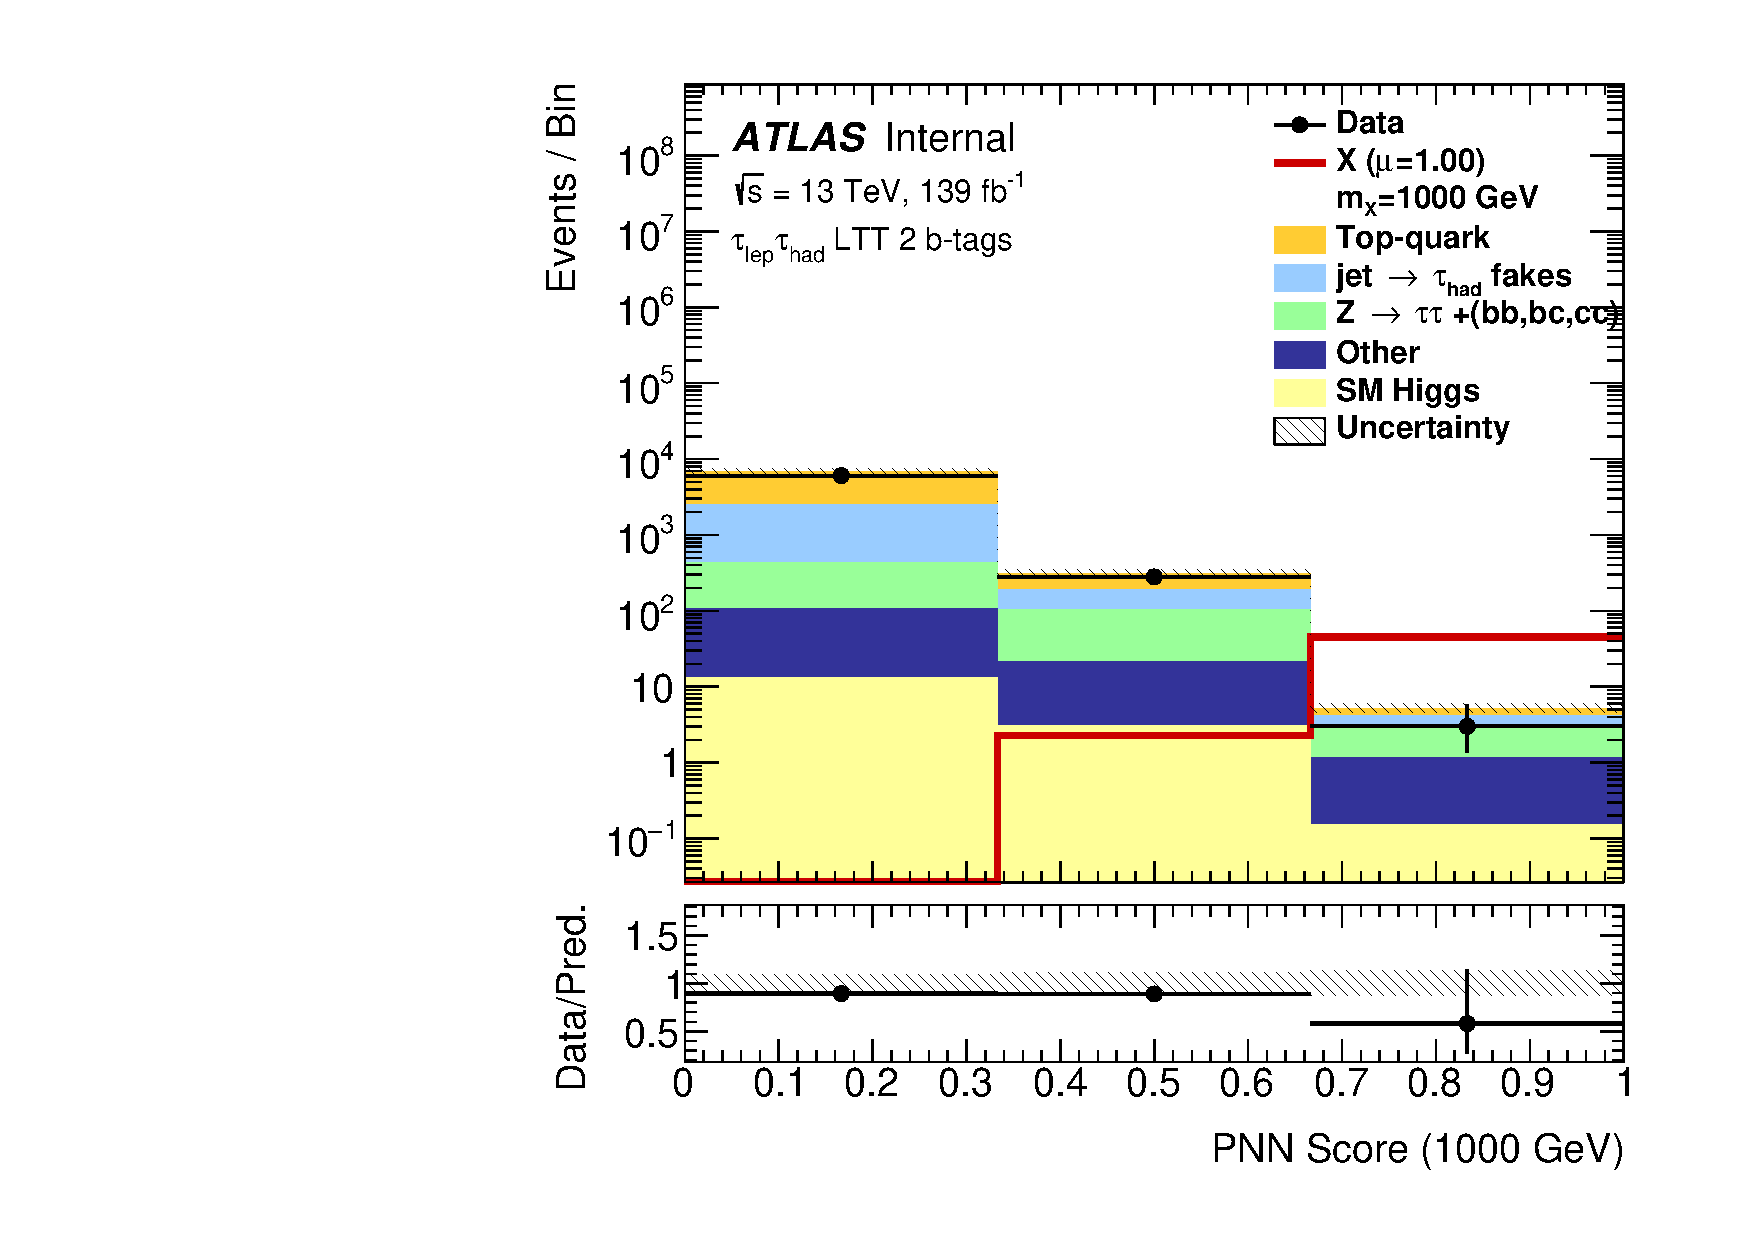
\includegraphics[width=.32\textwidth]{diHiggs/plots/MVA/LTT/Region_BMin0_incJet1_dist1000_J2_D2HDMPNN_T2_SpcTauLH_Y2015_LTT1_L1_Prefitlog.pdf} \\
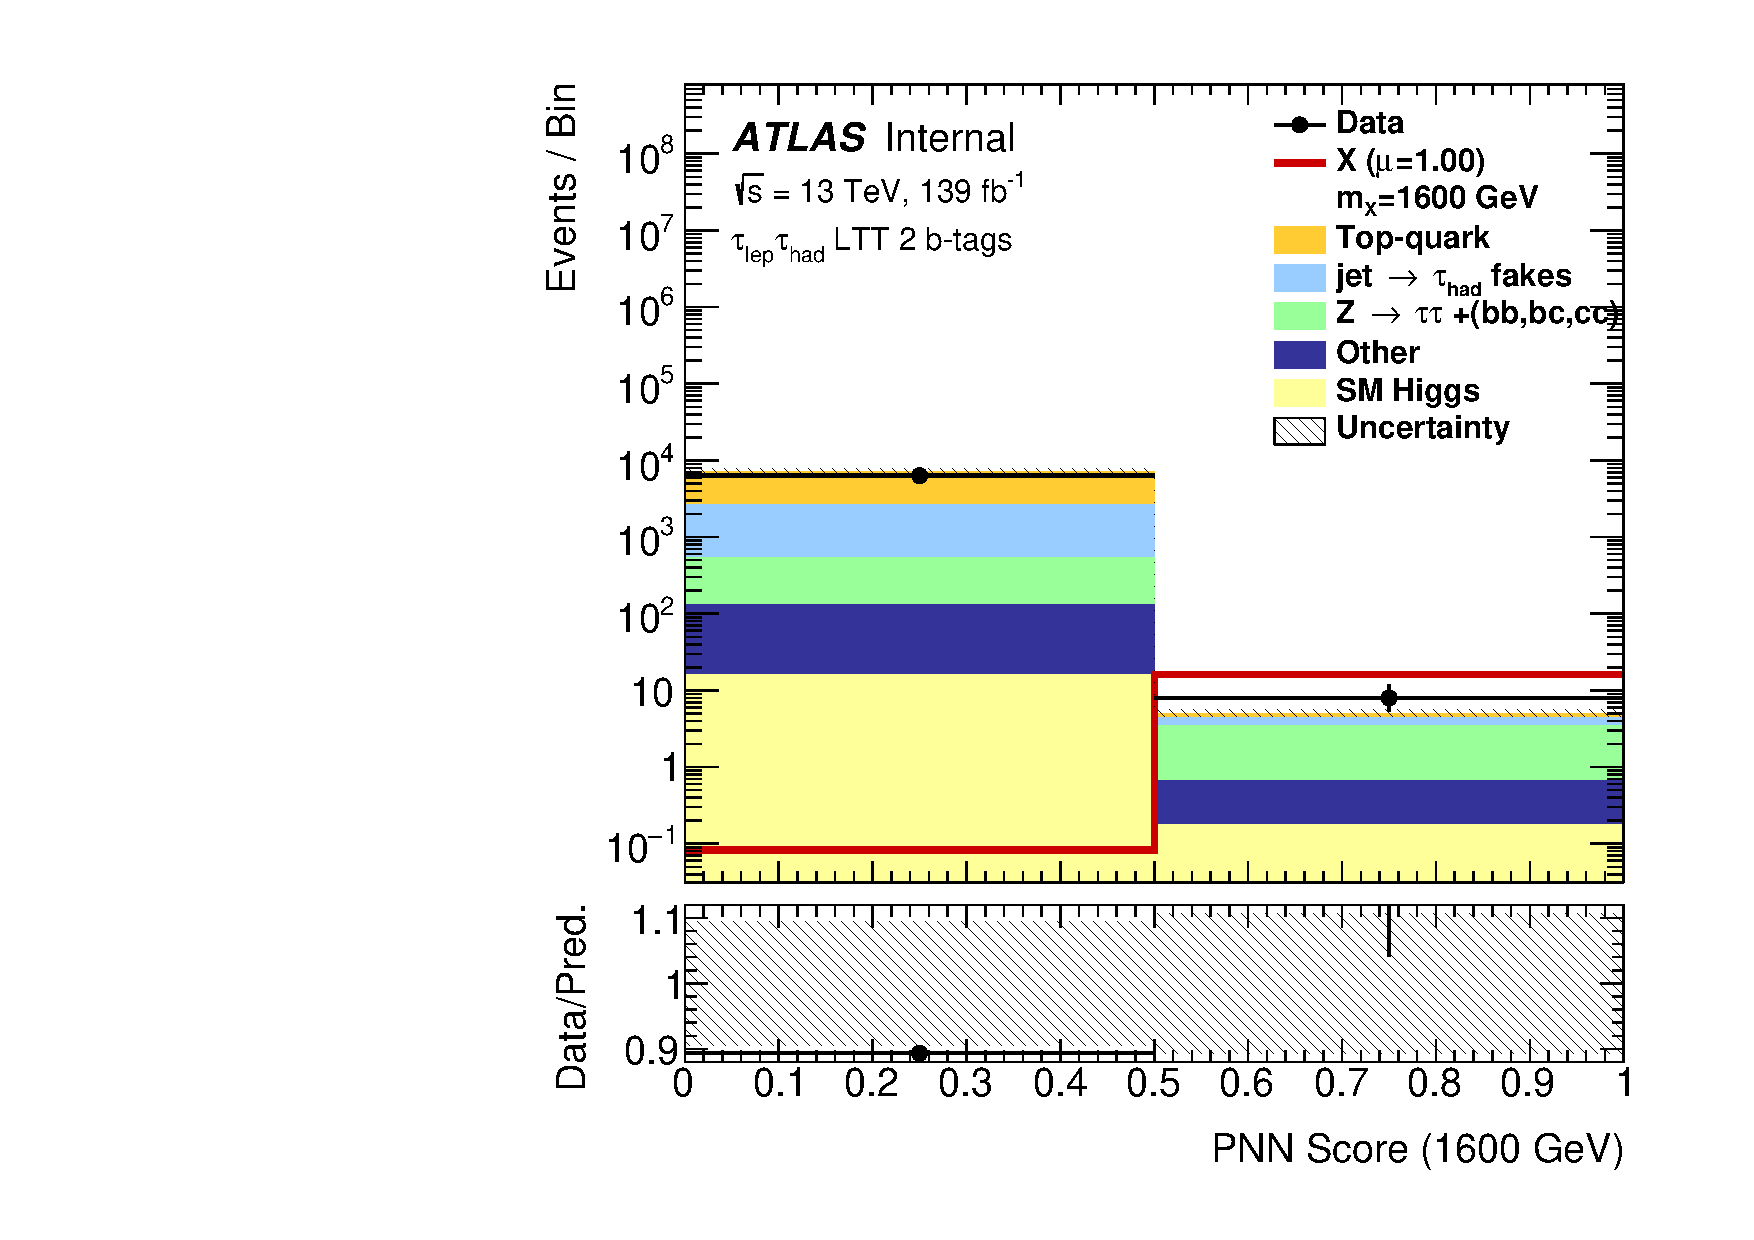
\includegraphics[width=.32\textwidth]{diHiggs/plots/MVA/LTT/Region_BMin0_incJet1_dist1600_J2_D2HDMPNN_T2_SpcTauLH_Y2015_LTT1_L1_Prefitlog.pdf} 
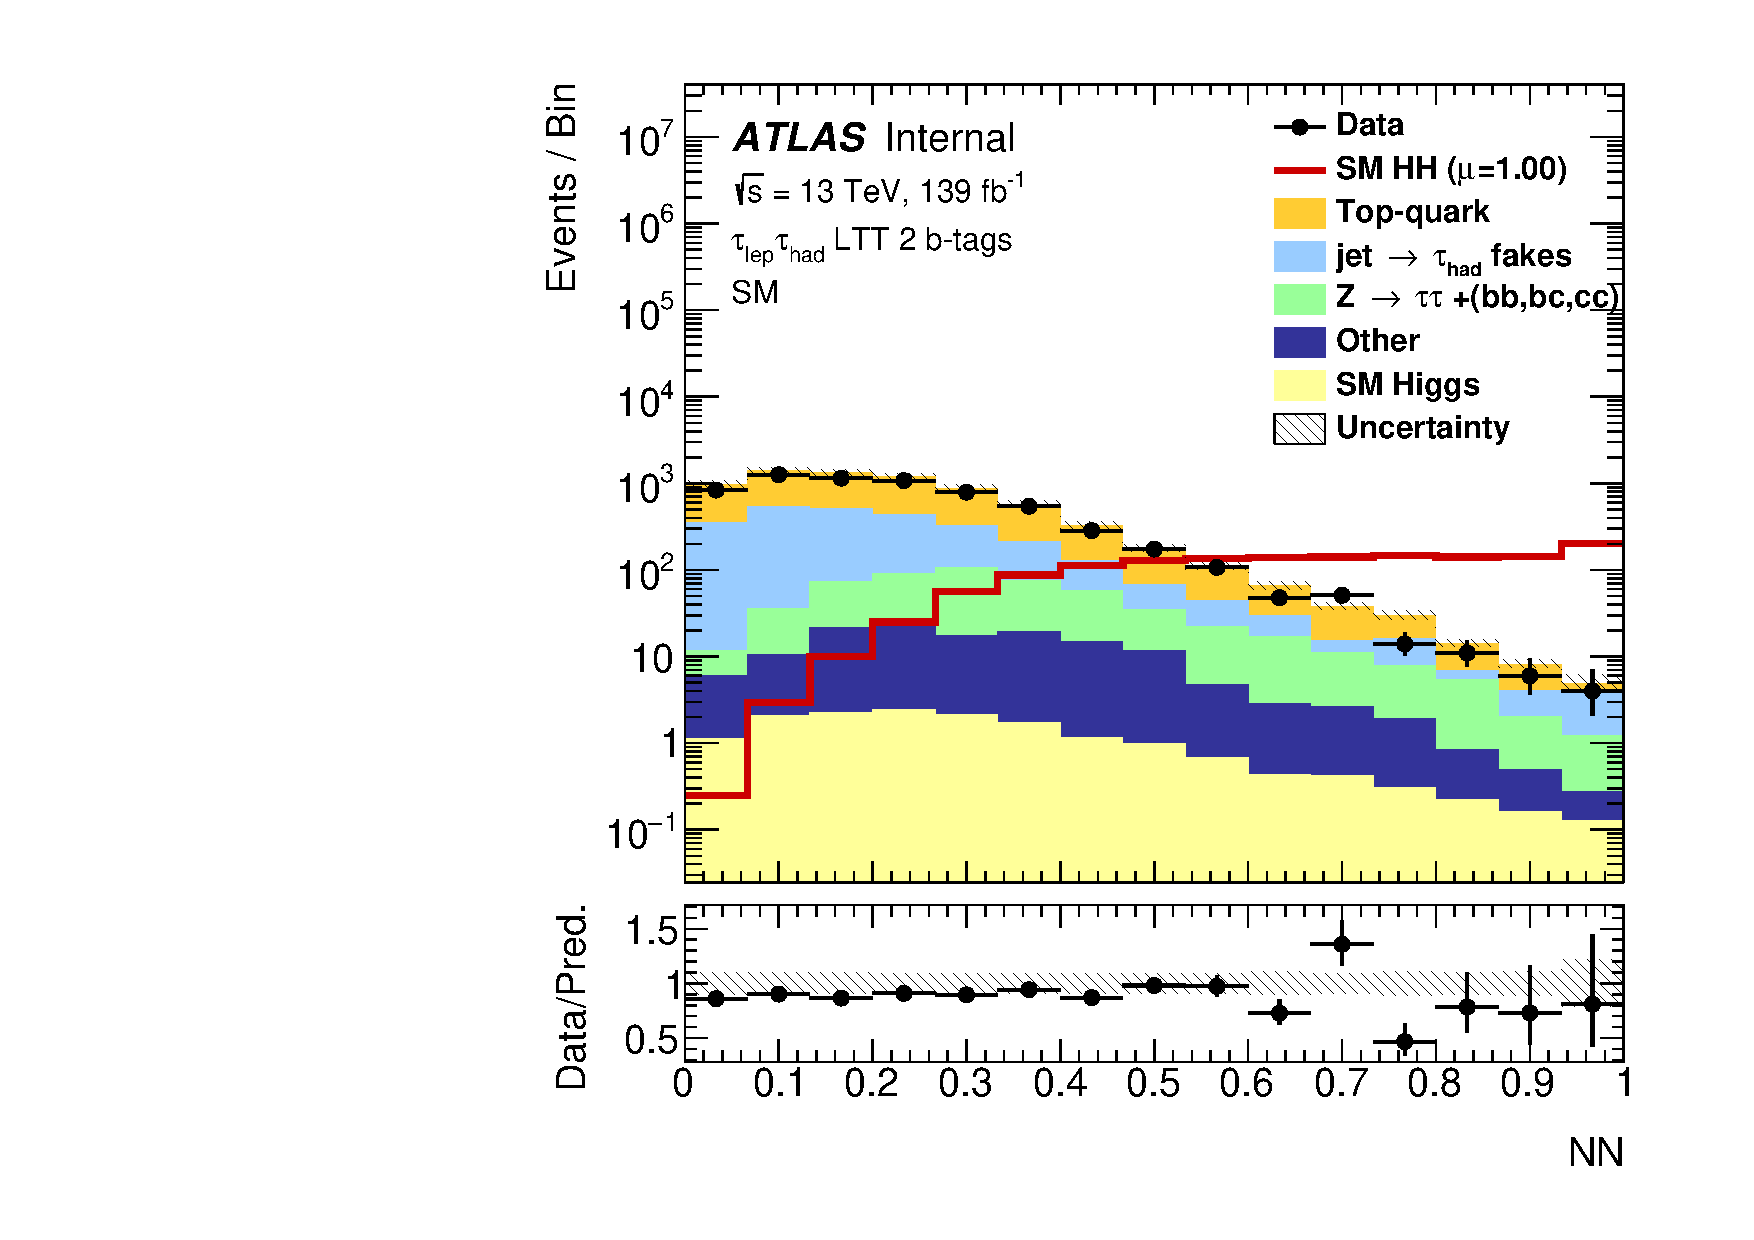
\includegraphics[width=.32\textwidth]{diHiggs/plots/MVA/LTT/Region_BMin0_incJet1_distNN_J2_DSM_T2_SpcTauLH_Y2015_LTT1_L1_Prefitlog.pdf}
\caption{Pre-fit PNN score distributions for the $300, 500, 1000, 1600$ GeV mass points and 
non-resonant NN in the di-Higgs $bb\lephad$ SLT (top two rows) and LTT (bottom two rows) signal regions.}
\label{fig:lephadmvaoutput}
\end{figure}
  


% Table~\ref{tab:yields_LastMVABin_LepHad_SLT},~\ref{tab:yields_LastMVABin_LepHad_LTT} 
% shows the event yields in the last three MVA bin of the SLT, LTT signal region respectively,
% which are the most significant bins for the signal extraction. Additionally,
% in~\ref{tab:significance_smbdt_bins_LepHad} the signal over
% background ratio and the signal significance is shown for all bins (as
% they enter the final fit) of the SMBDT distribution.


% The data versus MC distributions of these three variables are shown in 
% Figure~\ref{fig:MVAvariables}. 
% The distributions of the other MVA variables are shown in Appendix~\ref{}TODO: add plots in Appendix. 

% DiHiggs/plots/MVA/SLT_Final/HNone/BDTVarsPreselection/2

% \begin{figure}[htbp]
% \begin{subfigure}{.32\textwidth}
% \centering
% 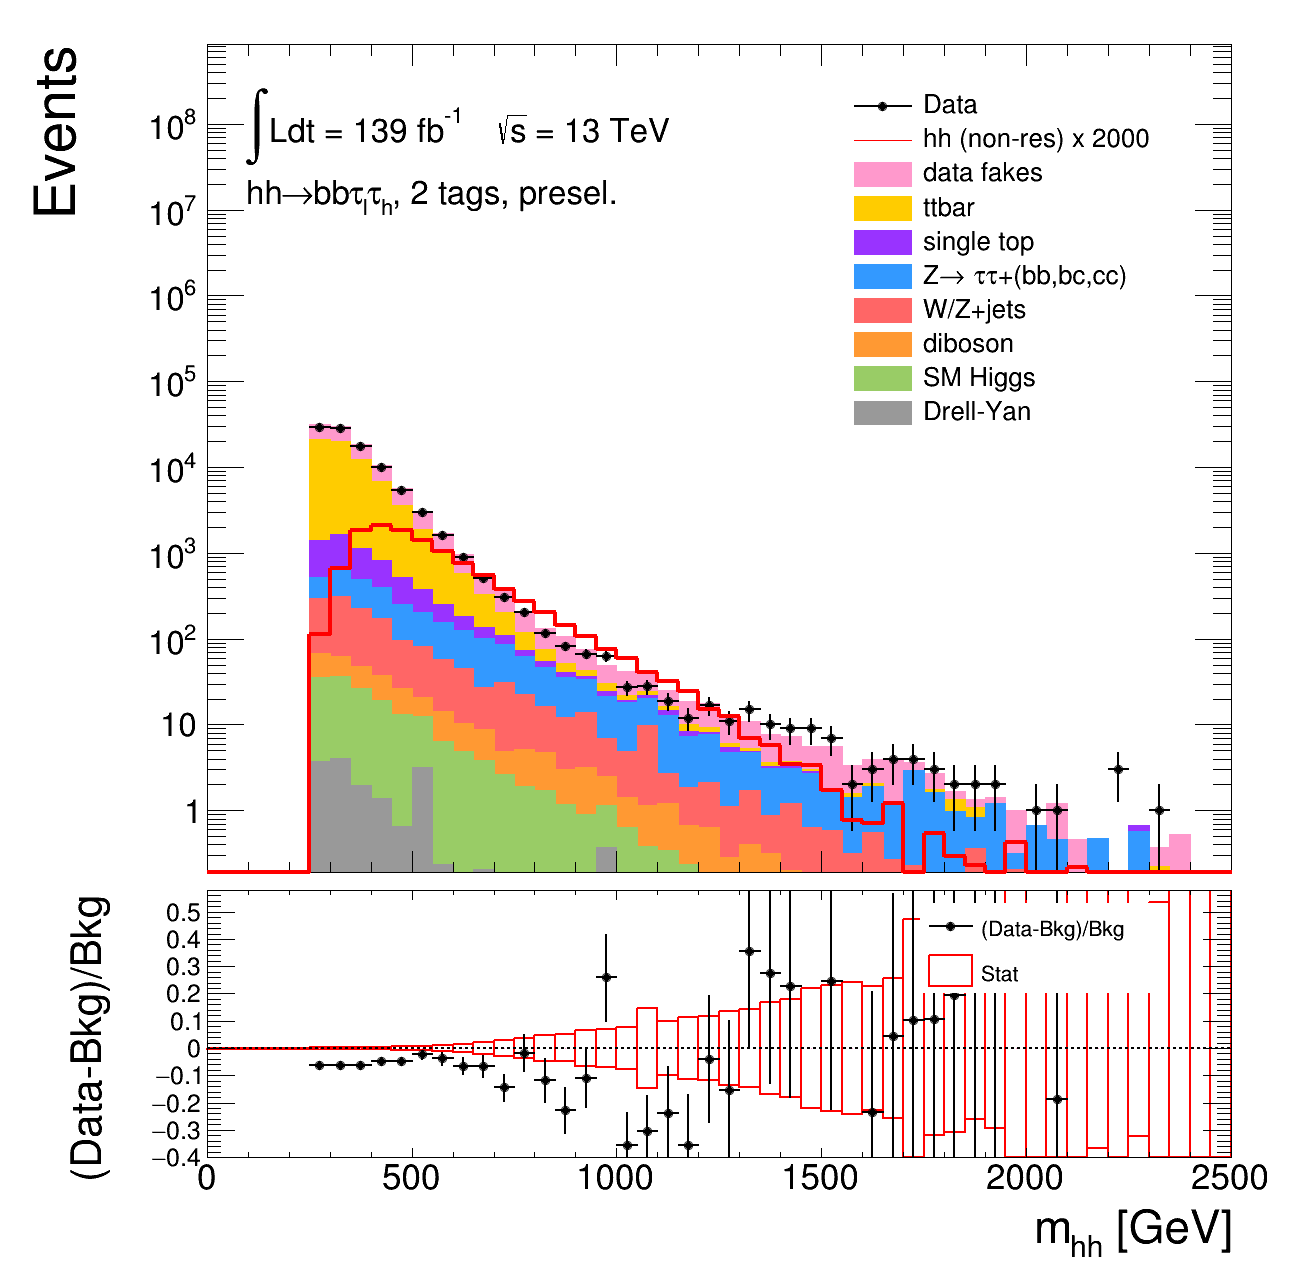
\includegraphics[width=0.85\linewidth]{DiHiggs/plots/MVA/SLT_Final/HNone/BDTVarsPreselection/2/C_2tag2pjet_0ptv_Mhh_Log.png}
% \caption{}
% \label{fig:MVAvariables:a}
% \end{subfigure}
% \begin{subfigure}{.32\textwidth}
% \centering
% 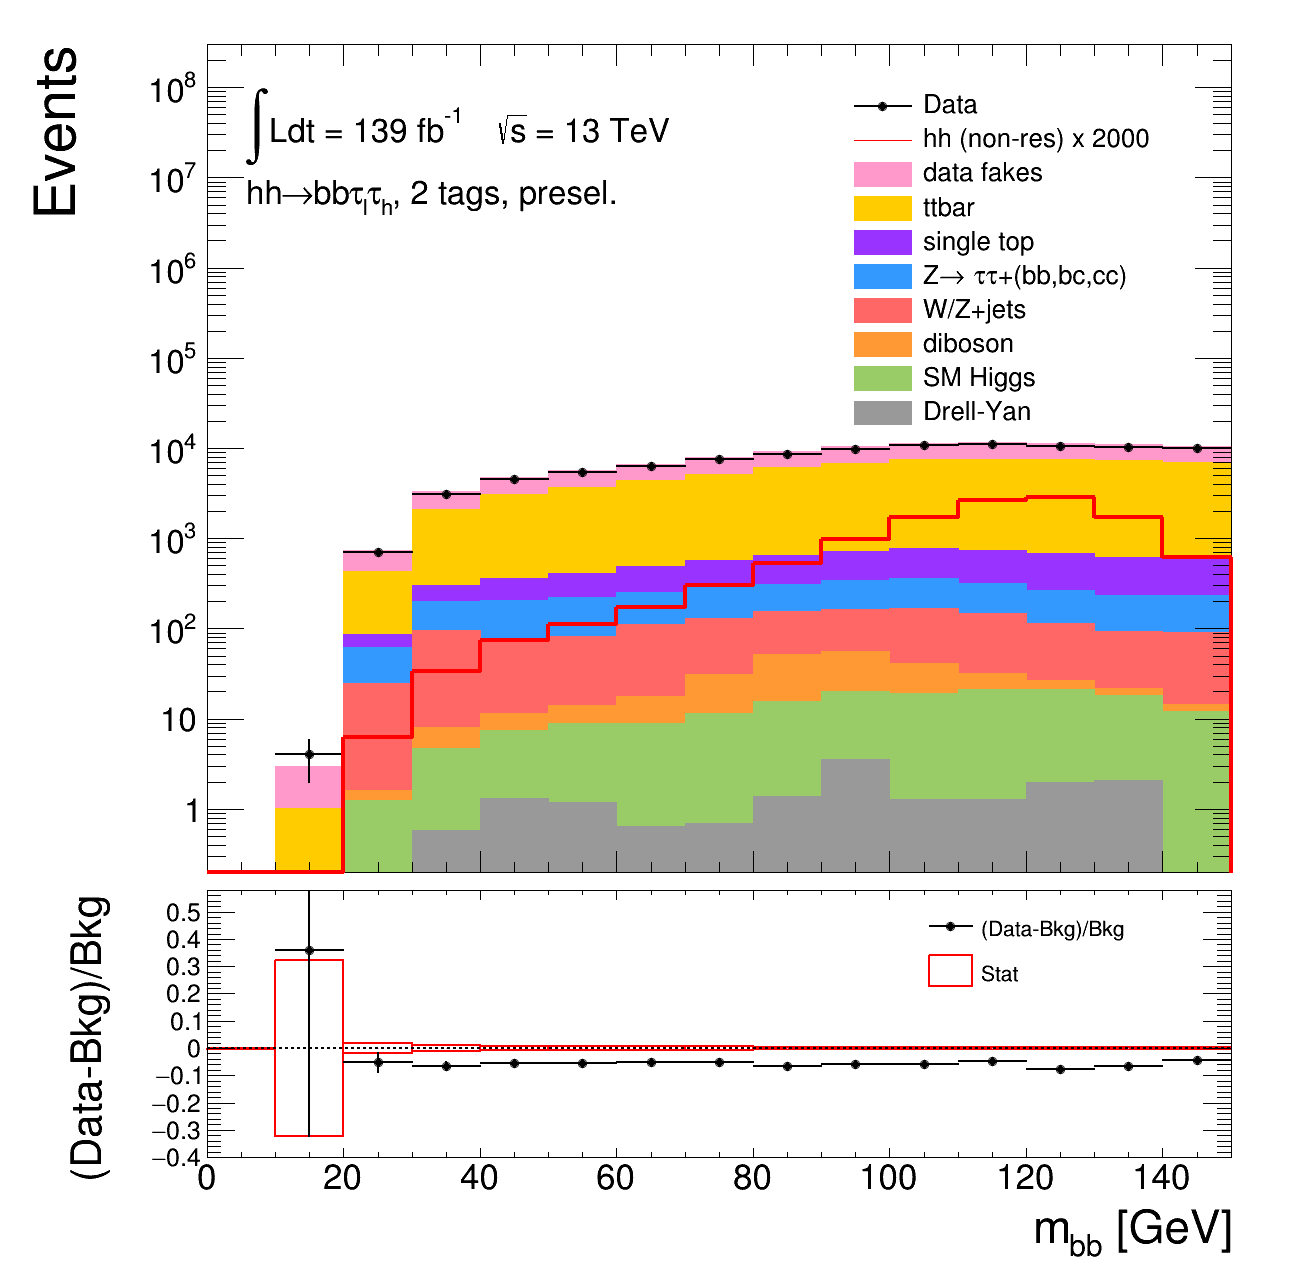
\includegraphics[width=0.85\linewidth]{DiHiggs/plots/MVA/SLT_Final/HNone/BDTVarsPreselection/2/C_2tag2pjet_0ptv_mbb_Log.png}
% \caption{}
% \label{fig:MVAvariables:b}
% \end{subfigure}
% \begin{subfigure}{.32\textwidth}
% \centering
% 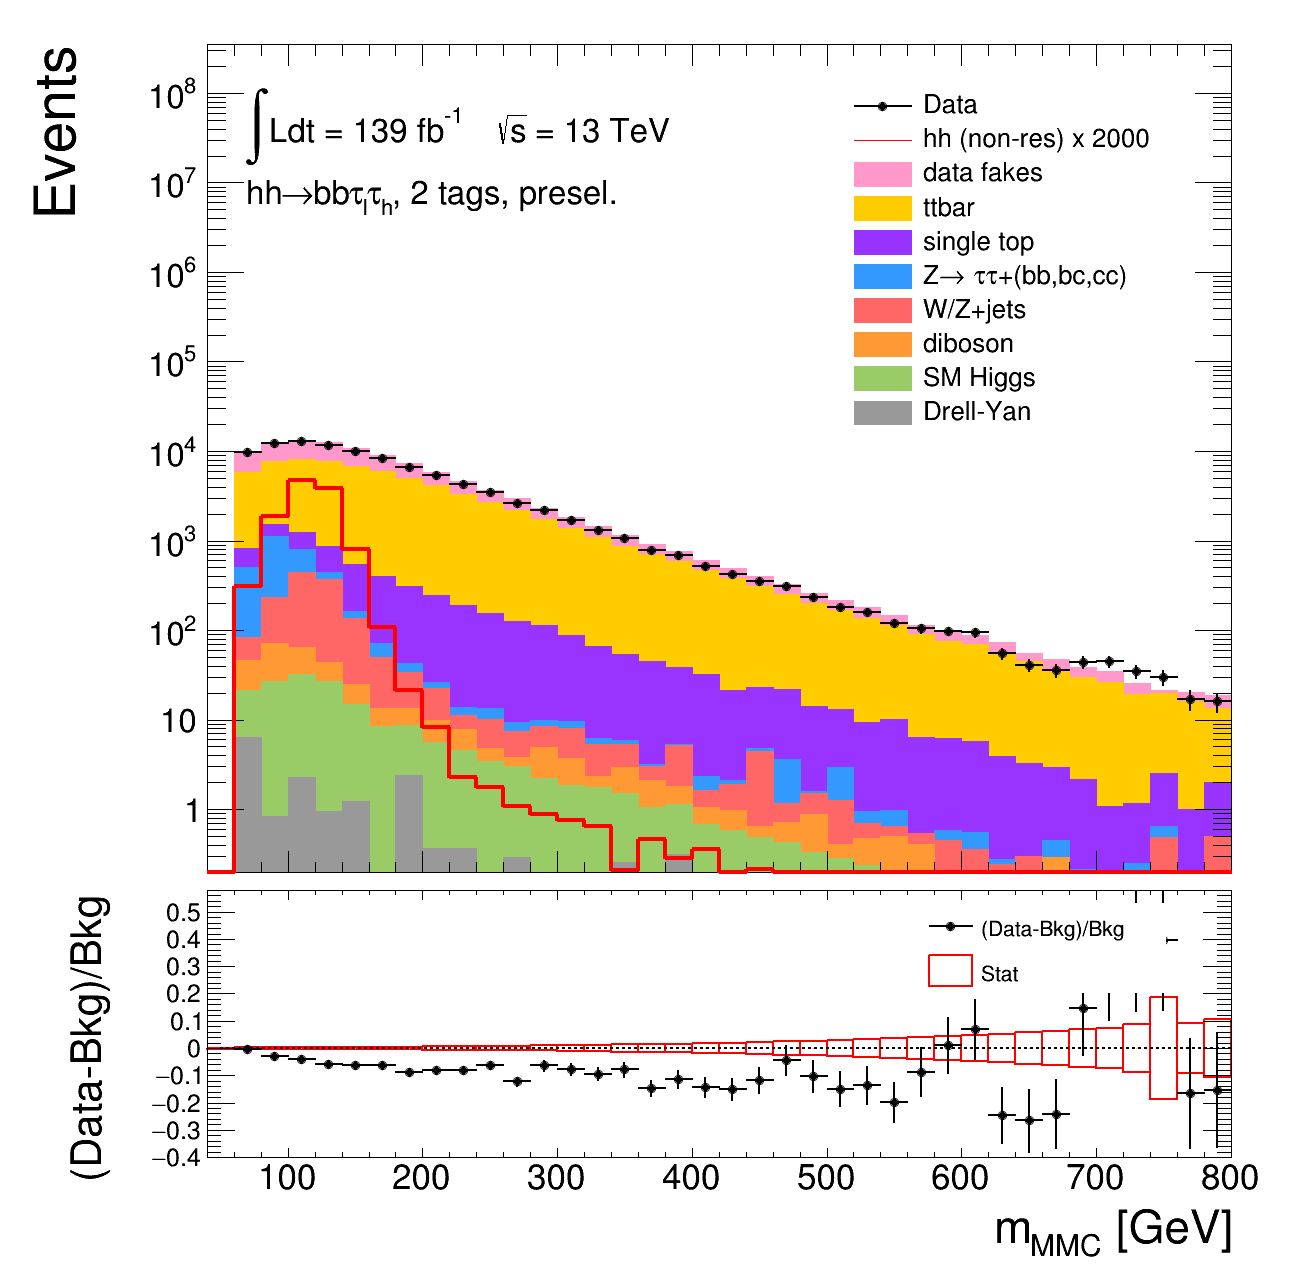
\includegraphics[width=0.85\linewidth]{DiHiggs/plots/MVA/SLT_Final/HNone/BDTVarsPreselection/2/C_2tag2pjet_0ptv_mMMC_Log.png}
% \caption{}
% \label{fig:MVAvariables:c}
% \end{subfigure}
% \\
% \begin{subfigure}{.32\textwidth}
% \centering
% 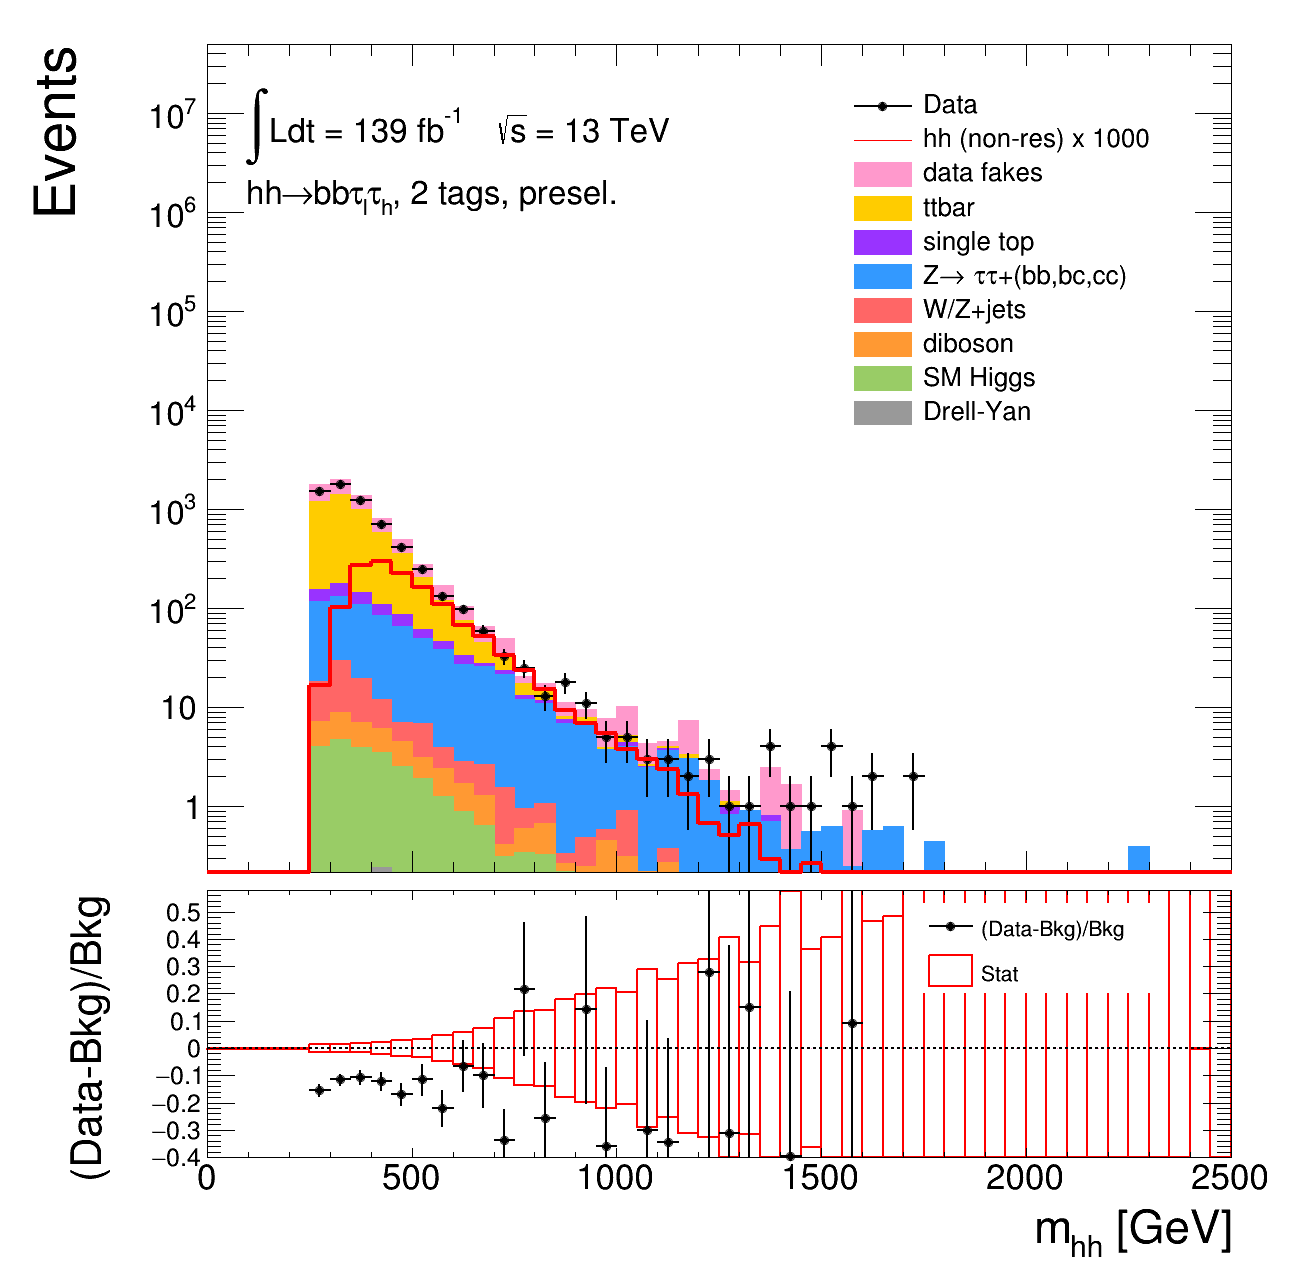
\includegraphics[width=0.85\linewidth]{DiHiggs/plots/MVA/LTT_Final/HNone/BDTVarsPreselection/2/C_2tag2pjet_0ptv_Mhh_Log.png}
% \caption{}
% \label{fig:MVAvariables:d}
% \end{subfigure}
% \begin{subfigure}{.32\textwidth}
% \centering
% 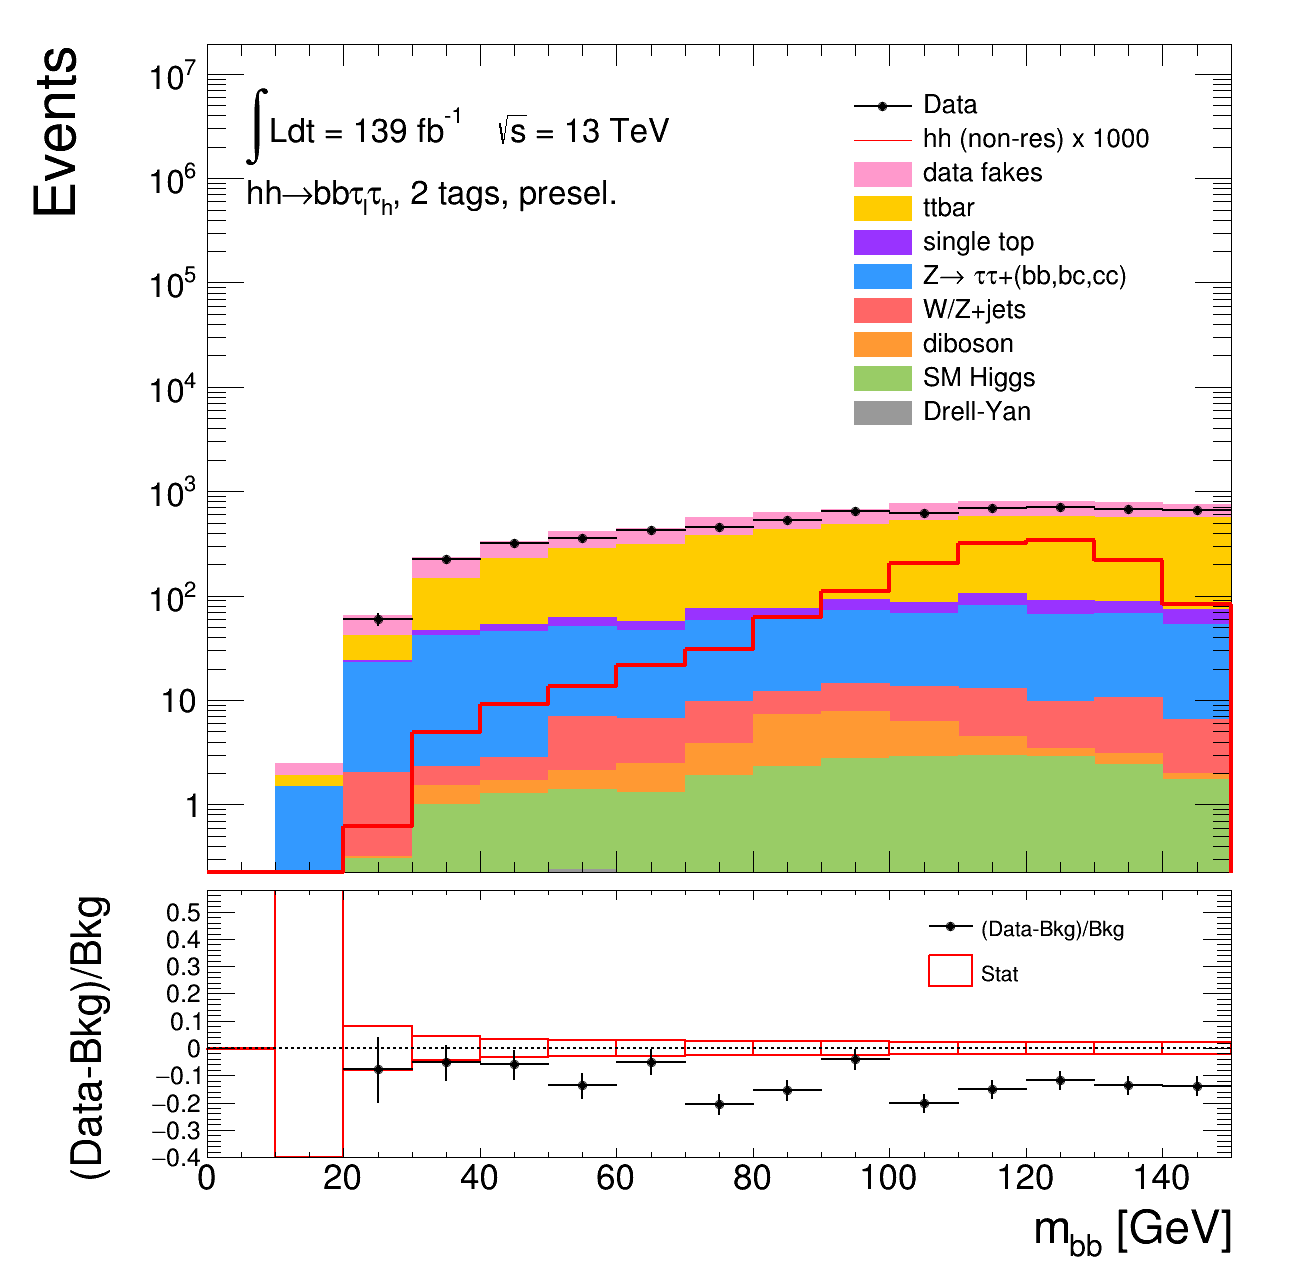
\includegraphics[width=0.85\linewidth]{DiHiggs/plots/MVA/LTT_Final/HNone/BDTVarsPreselection/2/C_2tag2pjet_0ptv_mbb_Log.png}
% \caption{}
% \label{fig:MVAvariables:e}
% \end{subfigure}
% \begin{subfigure}{.32\textwidth}
% \centering
% 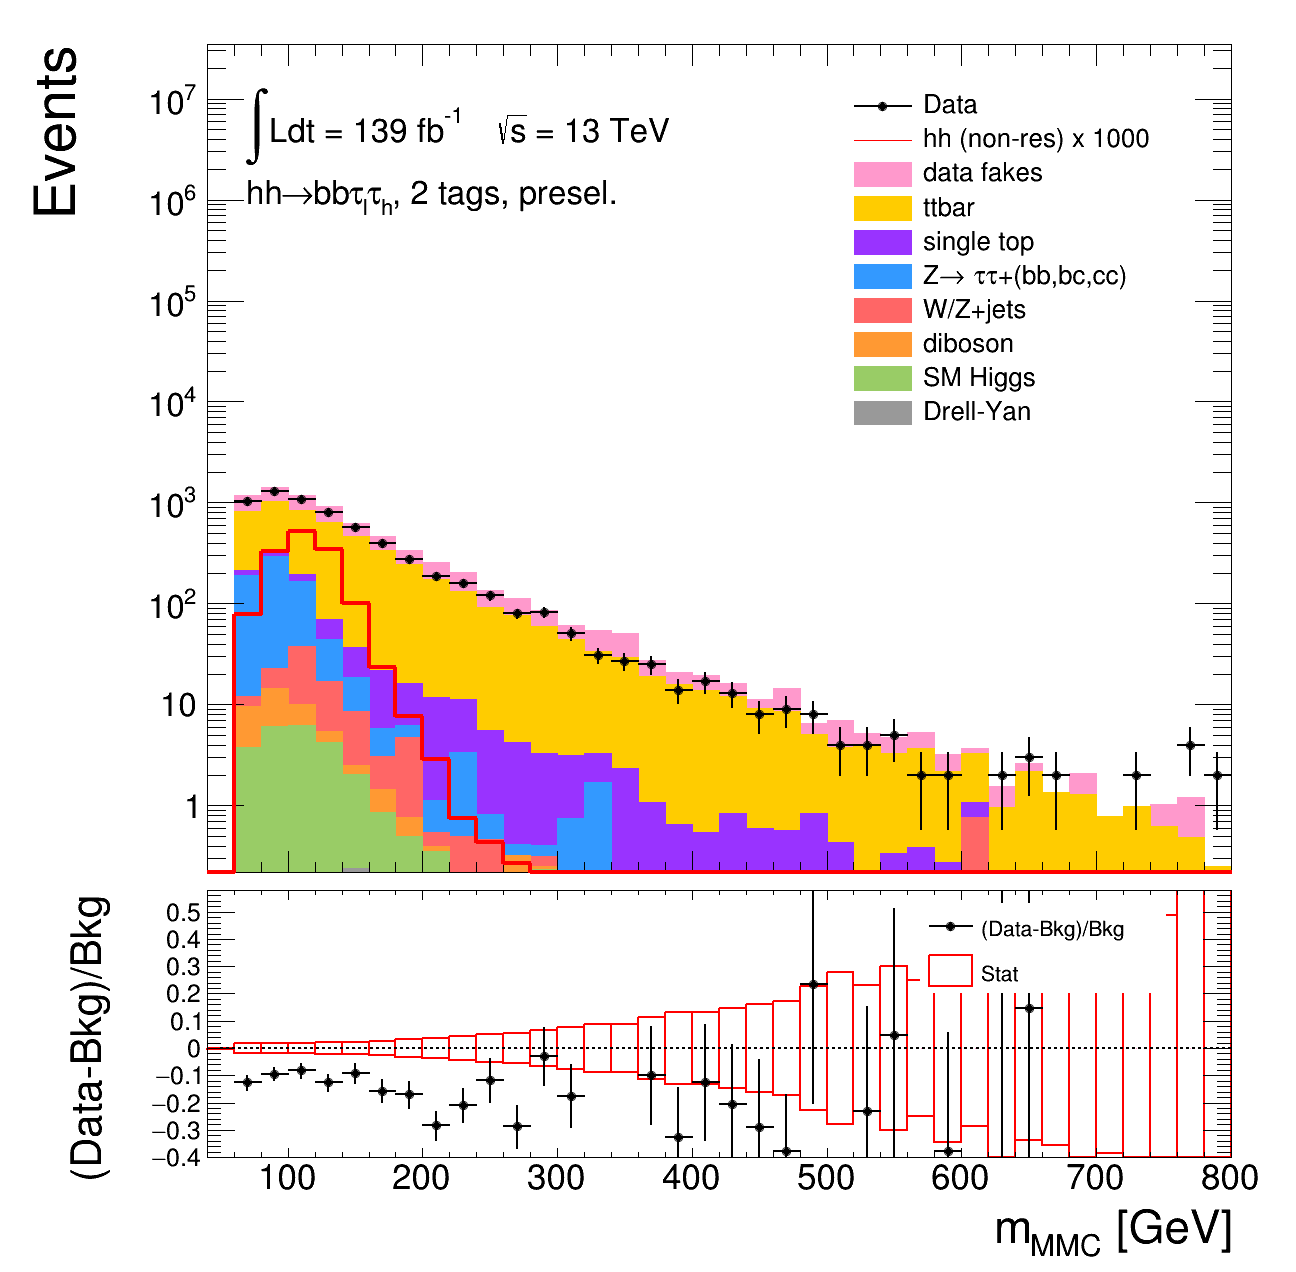
\includegraphics[width=0.85\linewidth]{DiHiggs/plots/MVA/LTT_Final/HNone/BDTVarsPreselection/2/C_2tag2pjet_0ptv_mMMC_Log.png}
% \caption{}
% \label{fig:MVAvariables:f}
% \end{subfigure}
% % location /hepstore/zhiyuan/Code_latest/run_Asimov/parametricnet/scripts/plots, run  python plot_mass.py to get
% \caption{
%     Showing the data versus MC distributions of the three most significant and discriminating variables, 
%     $m_{HH}$, $m_{\tau\tau}^\text{MMC}$ and $m_{bb}$, after the pre-selection and before applying the fit.  
%     The top (bottom) row is showing the variables in the SLT (LTT) channel. 
%     The non-resonant Di-Higgs signal is also included in the plots, and it is 
%     scaled by a factor of 2000 (1000) for the SLT (LTT) to make it more visible. 
%     The visible discrepancy between the data and MC is mostly due to the normalisation 
%     of the \ttbar\ background is not constrained.
%     In Section~\ref{sec:fit} TODO: add reference to fit section, the method used to
%     constrain the normalisation of the \ttbar\ and the Z + heavy flavour jets background 
%     is discussed.
%     The background in pink is the 
%     data-driven fakes which will be discussed in the following section~\ref{sec:DiHiggs:lephadfake}.
%     }
% \label{fig:MVAvariables}
% \end{figure}



